\documentclass[10pt]{article}

\usepackage{iftex}
\ifPDFTeX
  \errmessage{Please compile with XeLaTeX or LuaLaTeX}
\fi

\usepackage[fontset=fandol]{ctex}
\usepackage{fontspec}
\usepackage{geometry}
\usepackage{xcolor}
\usepackage{float}
\usepackage{microtype}
\usepackage{hyperref}
\usepackage{titlesec}
\usepackage{fancyhdr}
\usepackage{tikz}
\usetikzlibrary{positioning}
\usepackage[most]{tcolorbox}
\usepackage{amsmath,amssymb,amsthm,mathtools,bm}
\usepackage{enumitem}
\usepackage{booktabs}
\usepackage[capitalize,nameinlink]{cleveref}

\geometry{
  paperwidth=7.15in,
  paperheight=10in,
  left=0.55in,
  right=0.55in,
  top=0.6in,
  bottom=0.65in,
  headsep=0.24in,
  footskip=0.4in
}

\IfFontExistsTF{Times New Roman}{\setmainfont{Times New Roman}}{\setmainfont{TeX Gyre Termes}}
\IfFontExistsTF{Helvetica Neue}{\setsansfont{Helvetica Neue}}{\setsansfont{TeX Gyre Heros}}
\IfFontExistsTF{JetBrains Mono}{\setmonofont{JetBrains Mono}}{\IfFontExistsTF{Menlo}{\setmonofont{Menlo}}{\setmonofont{Courier New}}}
\IfFontExistsTF{Noto Serif CJK SC}{\setCJKmainfont{Noto Serif CJK SC}}{} 
\IfFontExistsTF{Noto Sans CJK SC}{\setCJKsansfont{Noto Sans CJK SC}}{} 

\linespread{1.15}
\setlength{\parindent}{1.6em}
\setlength{\parskip}{0.15em}

% 全局设置所有公式使用\displaystyle显示
\everymath{\displaystyle}
\everydisplay{\displaystyle}

\definecolor{brand}{HTML}{5B8CFF}
\definecolor{brandD}{HTML}{2F54EB}
\definecolor{ink}{HTML}{1A1A1A}
\definecolor{keybg}{HTML}{EFF4FF}
\definecolor{keydark}{HTML}{1F3C88}
\definecolor{accent}{HTML}{FFB84D}
\definecolor{accentD}{HTML}{FF8F1F}
\definecolor{soft}{HTML}{FFFBF2}
\definecolor{xhsRed}{HTML}{FF6B6B}
\definecolor{xhsDark}{HTML}{1F1F1F}
\definecolor{xhsCream}{HTML}{FFF8EE}
\definecolor{xhsBlue}{HTML}{3A86FF}
\definecolor{xhsYellow}{HTML}{FFC857}
\definecolor{secblue}{HTML}{365CFF}
\definecolor{thmBg}{RGB}{240,245,255}
\definecolor{lemBg}{RGB}{255,242,242}
\definecolor{defBg}{RGB}{240,247,255}

\hypersetup{
  colorlinks=true,
  linkcolor=brandD,
  citecolor=brandD,
  urlcolor=secblue,
  pdfauthor={用户名}, % 修改为你的名字
  pdftitle={文档标题} % 修改为你的文档标题
}

\newcounter{lecnum}
\renewcommand{\thesection}{\arabic{section}}
\renewcommand{\thesubsection}{\arabic{section}.\arabic{subsection}}
\renewcommand{\thesubsubsection}{\arabic{section}.\arabic{subsection}.\arabic{subsubsection}}
\renewcommand{\theequation}{\arabic{section}.\arabic{equation}}
\numberwithin{equation}{section}

\titleformat{\section}
  {\Large\bfseries\color{keydark}}
  {\thesection}{0.6em}{}
\titlespacing*{\section}{0pt}{1.1em}{0.45em}

\titleformat{\subsection}
  {\large\bfseries\color{brand}}
  {\thesubsection}{0.55em}{}
\titlespacing*{\subsection}{0pt}{0.9em}{0.3em}

\titleformat{\subsubsection}
  {\normalsize\bfseries\color{secblue}}
  {\thesubsubsection}{0.5em}{}
\titlespacing*{\subsubsection}{0pt}{0.7em}{0.2em}

\setlist[itemize]{leftmargin=1.5em,itemsep=0.25em,topsep=0.4em}
\setlist[enumerate]{leftmargin=1.7em,itemsep=0.25em,topsep=0.4em}

% 课程系列名称，可根据实际情况修改
\newcommand{\LectureSeries}{预备知识学习笔记}
% 主讲人名称，可根据实际情况修改
\newcommand{\LectureSpeaker}{Cabbage}
% 所属机构，可根据实际情况修改
\newcommand{\LectureAffiliation}{ECNU}

\fancyhf{}
\renewcommand{\headrulewidth}{0.4pt}
\fancyhead[L]{\small\sffamily\color{brandD}\LectureSeries}
\fancyhead[R]{\small\sffamily\color{ink}\nouppercase{\rightmark}}
\fancyfoot[L]{\small\sffamily\color{brand}\LectureSpeaker}
\fancyfoot[R]{\small\sffamily\color{brand}\arabic{page}}
\pagestyle{fancy}
\fancypagestyle{plain}{\pagestyle{fancy}}
\renewcommand{\sectionmark}[1]{\markright{#1}}

\tcbset{
  cn-panel/.style={
    enhanced,
    breakable,
    boxrule=0.7pt,
    arc=4pt,
    left=10pt,right=10pt,top=10pt,bottom=10pt
  },
  cn-soft/.style={
    enhanced,
    breakable,
    frame hidden,
    borderline west={3pt}{0pt}{#1},
    colback=#1!8,
    left=9pt,right=9pt,top=8pt,bottom=8pt,
    arc=2pt
  }
}

\newcommand{\LectureBanner}[6]{%
  \setcounter{lecnum}{#1}%
  \markright{#2}%
  \begin{tcolorbox}[
    cn-panel,
    colback=keybg,
    colframe=brandD,
    borderline west={4pt}{0pt}{accent}
  ]
    {\sffamily\small\color{ink!60} #4 \hfill #5}\par
    \vspace{0.35em}
    {\bfseries\fontsize{22}{26}\selectfont\color{keydark} Chapter #1：#2\par}
    \vspace{0.2em}
    {\large\color{brand} #3\par}
    \vspace{0.7em}
    {\small\sffamily\color{ink!72} Author：#6 \hfill {\color{brandD}\LectureAffiliation}}
  \end{tcolorbox}
  \vspace{0.7em}
}

\newtcolorbox{SummaryBox}{
  cn-panel,
  colback=xhsCream,
  colframe=accent,
  title=\textbf{本讲摘要},
  fonttitle=\bfseries,
  coltitle=white,
  colbacktitle=accent
}

\newtcolorbox{AnalysisBox}{
  cn-soft=secblue,
  title=\textbf{分析},
  fonttitle=\bfseries,
  coltitle=secblue
}

\newtcolorbox{RemarkBox}{
  cn-soft=accentD,
  title=\textbf{备注},
  fonttitle=\bfseries,
  coltitle=accentD
}

\newtcolorbox{ExampleBox}{
  cn-panel,
  colback=soft,
  colframe=xhsBlue,
  title=\textbf{Example},
  fonttitle=\bfseries,
  coltitle=white,
  colbacktitle=xhsBlue
}

\usepackage{listings}

\lstdefinestyle{PythonStyle}{
  language=Python,
  basicstyle=\ttfamily\scriptsize,
  keywordstyle=\color{blue!70},
  stringstyle=\color{green!60},
  commentstyle=\color{red!60!green},
  numbers=left,
  numberstyle=\tiny\color{gray},
  breaklines=true,
  breakatwhitespace=true,
  tabsize=4,
  showstringspaces=false,
  frame=single,
  framesep=3pt,
  framexleftmargin=3pt,
  xleftmargin=10pt
}

\newtcolorbox{OutputBox}{
  cn-panel,
  colback=black!5,
  colframe=gray!30,
  title=\textbf{执行输出：},
  fonttitle=\bfseries\small,
  coltitle=black,
  left=2mm, right=2mm, top=2mm, bottom=2mm
}

\newtcolorbox{CodeBox}{
  cn-panel,
  colback=xhsDark!5,
  colframe=brand,
  title=\textbf{Python 代码实现},
  fonttitle=\bfseries,
  coltitle=white,
  colbacktitle=brand,
  enhanced,
  breakable
}

\theoremstyle{plain}
\newtheorem{theorem}{定理}[section]
\newtheorem{lemma}[theorem]{引理}
\newtheorem{proposition}[theorem]{命题}
\newtheorem{corollary}[theorem]{推论}
\theoremstyle{definition}
\newtheorem{definition}[theorem]{定义}
\theoremstyle{remark}
\newtheorem{remark}[theorem]{注}

\tcolorboxenvironment{theorem}{cn-panel,colback=thmBg,colframe=secblue,borderline west={3pt}{0pt}{secblue}}
\tcolorboxenvironment{lemma}{cn-panel,colback=lemBg,colframe=accentD,borderline west={3pt}{0pt}{accentD}}
\tcolorboxenvironment{proposition}{cn-panel,colback=thmBg,colframe=brandD,borderline west={3pt}{0pt}{brandD}}
\tcolorboxenvironment{corollary}{cn-panel,colback=defBg,colframe=brand,borderline west={3pt}{0pt}{brand}}
\tcolorboxenvironment{definition}{cn-soft=brandD,title=\textbf{定义},fonttitle=\bfseries,coltitle=brandD}
\tcolorboxenvironment{remark}{cn-soft=accentD,title=\textbf{注},fonttitle=\bfseries,coltitle=accentD}

% 数学符号定义，可根据需要添加或修改
\DeclareMathOperator{\diam}{diam}
\newcommand{\E}{\mathbb{E}}
\newcommand{\R}{\mathbb{R}}
\newcommand{\ip}[2]{\left\langle #1, #2 \right\rangle}
\newcommand{\norm}[1]{\lVert #1 \rVert}
\newcommand{\grad}[1]{\nabla #1}

\renewcommand{\baselinestretch}{1.05}
\begin{document}

% 目录页
\clearpage
\pagestyle{plain}
\begin{tcolorbox}[
		cn-panel,
		colback=keybg,
		colframe=brandD,
		borderline west={4pt}{0pt}{accent},
		title=\textbf{目录},
		fonttitle=\bfseries,
		coltitle=white,
		colbacktitle=brandD
	]
	\tableofcontents
\end{tcolorbox}
\vspace{0.7em}
\clearpage

% 第一讲
\setcounter{section}{1}
\setcounter{subsection}{0}
\addcontentsline{toc}{section}{Chapter 1:梯度下降算法}
\LectureBanner
{1} % 修改为讲座编号
{梯度下降算法} % 修改为讲座标题
{理论基础与实现} % 修改为讲座副标题
{大模型学习笔记} % 修改为课程系列名称
{2026 Spring} % 修改为学期信息
{Cabbage} % 修改为主讲人姓名

\begin{SummaryBox}
	本讲详细介绍了梯度下降算法的精确定义、核心定理及其证明，并提供了可直接运行的Python代码实现。梯度下降是最基础且广泛应用的优化算法，通过沿着负梯度方向迭代更新参数，逐步逼近目标函数的最小值。
\end{SummaryBox}
\setcounter{subsection}{0}
% 线性代数基础
\subsection{线性代数基础}

本文覆盖实对称矩阵特征值性质、实对称矩阵合同对角化、从多元泰勒展开到凸函数二阶条件的完整推导三大知识点，所有推导从基础定义出发，先明确定义再陈述定理、给出证明，符号体系统一为：$\R^n$ 表示 n 维实向量空间，$\R^{n\times n}$ 表示 n 阶实方阵，$D\subset\R^n$ 表示 n 元函数的定义域。

\subsubsection{实对称阵的特征值一定是实数}

{\par\vspace{0.8ex}\noindent\normalsize\bfseries\color{secblue} 相关名词定义\par}

{\par\vspace{0.8ex}\noindent\normalsize\bfseries\color{secblue} （1）实对称矩阵\par}

设 $A\in\R^{n\times n}$，若 $A$ 的转置等于自身，即 $A^T=A$，则称 $A$ 为实对称矩阵（注：若无特殊说明，"对称阵" 均指实对称矩阵，复对称阵无此性质，复域中对应埃尔米特矩阵）。

{\par\vspace{0.8ex}\noindent\normalsize\bfseries\color{secblue} （2）特征值与特征向量\par}

设 $A\in\R^{n\times n}$，若存在复数 $\lambda$ 和非零复向量 $x\in\mathbb{C}^n$，使得 $Ax=\lambda x$，则称 $\lambda$ 为 $A$ 的特征值，非零向量 $x$ 为 $A$ 对应于 $\lambda$ 的特征向量（特征向量必非零，这是定义核心）。

{\par\vspace{0.8ex}\noindent\normalsize\bfseries\color{secblue} （3）复数的共轭与复向量的共轭转置\par}

对复数 $a+bi$，其共轭记为 $\overline{a+bi}=a-bi$；对复向量 $x=(x_1,x_2,\ldots,x_n)^T\in\mathbb{C}^n$，其共轭为 $\overline{x}=(\overline{x_1},\overline{x_2},\ldots,\overline{x_n})^T$。

复向量的共轭转置记为 $x^H=(\overline{x})^T$，实向量的共轭转置等价于普通转置（$x^H=x^T$）。

{\par\vspace{0.8ex}\noindent\normalsize\bfseries\color{secblue} （4）复向量的内积\par}

对 $x,y\in\mathbb{C}^n$，内积定义为 $\langle x,y\rangle=x^H y$，若 $x\neq 0$，则 $\langle x,x\rangle=\sum_{i=1}^n |x_i|^2 > 0$（模的平方和，恒正）。

{\par\vspace{0.8ex}\noindent\normalsize\bfseries\color{secblue} 定理准确陈述\par}

\begin{theorem}
	设 $A\in\R^{n\times n}$ 为实对称矩阵，则 $A$ 的所有特征值均为实数。
\end{theorem}

{\par\vspace{0.8ex}\noindent\normalsize\bfseries\color{secblue} 严格证明（从定义出发）\par}

设 $\lambda$ 为实对称阵 $A$ 的任意一个特征值，$x\in\mathbb{C}^n$ 是对应于 $\lambda$ 的非零特征向量，则由特征值定义有：
\begin{equation}
	Ax=\lambda x
\end{equation}

{\par\vspace{0.8ex}\noindent\normalsize\bfseries\color{secblue} 步骤 1：对等式 (1) 两边取共轭\par}

因 $A$ 是实矩阵，其元素均为实数，故 $\overline{A}=A$；对等式两边共轭得：
\begin{equation}
	\overline{Ax}=\overline{\lambda x}\implies\overline{A}\overline{x}=\overline{\lambda}\overline{x}\implies A\overline{x}=\overline{\lambda}\overline{x}
\end{equation}

{\par\vspace{0.8ex}\noindent\normalsize\bfseries\color{secblue} 步骤 2：对等式 (1) 两边取共轭转置\par}

共轭转置满足 $(AB)^H=B^H A^H$，且 $A$ 是实对称阵，故 $A^H=(\overline{A})^T=A^T=A$，对 (1) 取共轭转置得：
\begin{equation}
	(Ax)^H=(\lambda x)^H\implies x^H A^H=\overline{\lambda} x^H\implies x^H A=\overline{\lambda} x^H
\end{equation}

{\par\vspace{0.8ex}\noindent\normalsize\bfseries\color{secblue} 步骤 3：对等式 (3) 两边右乘 $x$，结合特征值定义化简\par}

\begin{equation}
	x^H Ax=\overline{\lambda} x^H x
\end{equation}

由 (1) 知 $Ax=\lambda x$，代入 (4) 左边得：
\begin{equation}
	x^H\cdot\lambda x=\overline{\lambda} x^H x\implies\lambda x^H x=\overline{\lambda} x^H x
\end{equation}

{\par\vspace{0.8ex}\noindent\normalsize\bfseries\color{secblue} 步骤 4：利用复向量内积的正定性推导 $\lambda=\overline{\lambda}$\par}

因 $x$ 是特征向量，故 $x\neq 0$，由复向量内积定义得 $x^H x=\sum_{i=1}^n |x_i|^2 > 0$，对 (5) 两边同时除以 $x^H x$ 得：
\[\lambda=\overline{\lambda}\]

一个复数等于其共轭，当且仅当该复数为实数，故实对称阵的任意特征值均为实数。

\begin{corollary}
	实对称阵的特征向量均可取为实向量（因特征值为实数，特征方程 $(A-\lambda E)x=0$ 是实系数线性方程组，必有实非零解）。
\end{corollary}

\subsubsection{实对称阵一定存在相合（合同）对角化：$Q^T AQ=\Lambda$}

{\par\vspace{0.8ex}\noindent\normalsize\bfseries\color{secblue} 相关名词定义\par}

{\par\vspace{0.8ex}\noindent\normalsize\bfseries\color{secblue} （1）矩阵的合同（相合）\par}

设 $A,B\in\R^{n\times n}$，若存在 n 阶实可逆矩阵 $C$，使得 $C^T AC=B$，则称矩阵 $A$ 与 $B$ 合同（相合），称 $C$ 为合同变换矩阵；若 $C$ 为正交矩阵，则称 $A$ 与 $B$ 正交合同。

{\par\vspace{0.8ex}\noindent\normalsize\bfseries\color{secblue} （2）可逆矩阵\par}

设 $A\in\R^{n\times n}$，若存在 $B\in\R^{n\times n}$，使得 $AB=BA=E$（$E$ 为 n 阶单位阵），则称 $A$ 可逆，$B$ 为 $A$ 的逆矩阵，记为 $A^{-1}$；方阵可逆的充要条件是 $\det(A)\neq 0$（行列式非零）。

{\par\vspace{0.8ex}\noindent\normalsize\bfseries\color{secblue} （3）正交矩阵\par}

设 $Q\in\R^{n\times n}$，若 $Q^T Q=QQ^T =E$，则称 $Q$ 为正交矩阵；正交矩阵的核心性质：$Q^T=Q^{-1}$（逆等于转置），且 $\det(Q)=\pm 1$（必可逆）。

{\par\vspace{0.8ex}\noindent\normalsize\bfseries\color{secblue} （4）对角矩阵\par}

设 $\Lambda\in\R^{n\times n}$，若 $\Lambda$ 的非对角线元素均为 0，即 \[\Lambda=\text{diag}(\lambda_1,\lambda_2,\ldots,\lambda_n)=\begin{pmatrix}\lambda_1 & 0 & \cdots & 0\\ 0 & \lambda_2 & \cdots & 0\\ \vdots & \vdots & \ddots & \vdots\\ 0 & 0 & \cdots & \lambda_n\end{pmatrix}\]，则称 $\Lambda$ 为对角矩阵。

{\par\vspace{0.8ex}\noindent\normalsize\bfseries\color{secblue} （5）矩阵的相似\par}

设 $A,B\in\R^{n\times n}$，若存在 n 阶实可逆矩阵 $P$，使得 $P^{-1} AP=B$，则称 $A$ 与 $B$ 相似；若 $P$ 为正交矩阵，则称 $A$ 与 $B$ 正交相似。

{\par\vspace{0.8ex}\noindent\normalsize\bfseries\color{secblue} 定理准确陈述\par}

\begin{theorem}
	设 $A\in\R^{n\times n}$ 为实对称矩阵，则存在 n 阶正交矩阵 $Q$，使得 $Q^T AQ=\Lambda$，其中 $\Lambda=\text{diag}(\lambda_1,\lambda_2,\ldots,\lambda_n)$，$\lambda_1,\lambda_2,\ldots,\lambda_n$ 为 $A$ 的全部特征值。
\end{theorem}

\begin{corollary}
	实对称阵必可正交合同对角化，且合同变换矩阵可取正交矩阵（正交合同是合同的特殊情况，故实对称阵必可普通合同对角化）。
\end{corollary}

{\par\vspace{0.8ex}\noindent\normalsize\bfseries\color{secblue} 严格证明（从定义出发，分两步）\par}

实对称阵的合同对角化基于其正交相似对角化，而正交相似对角化又基于实对称阵的特征向量正交性，证明分两步：先证实对称阵的不同特征值的特征向量正交，再构造正交矩阵完成对角化。

{\par\vspace{0.8ex}\noindent\normalsize\bfseries\color{secblue} 步骤 1：证明实对称阵不同特征值的特征向量相互正交\par}

设 $\lambda_1,\lambda_2$ 为实对称阵 $A$ 的两个不同特征值，$x_1,x_2$ 为对应的实特征向量（由第一部分推论，特征向量可取实向量），则：
\[Ax_1=\lambda_1 x_1,\quad Ax_2=\lambda_2 x_2\]

对 $Ax_1=\lambda_1 x_1$ 两边取转置得：
\[x_1^T A^T=\lambda_1 x_1^T\]
因 $A^T=A$，故 $x_1^T A=\lambda_1 x_1^T$。

两边右乘 $x_2$ 得：
\[x_1^T Ax_2=\lambda_1 x_1^T x_2\]
代入 $Ax_2=\lambda_2 x_2$ 得：
\[\lambda_2 x_1^T x_2=\lambda_1 x_1^T x_2\implies(\lambda_1-\lambda_2)x_1^T x_2=0\]

因 $\lambda_1\neq\lambda_2$，故 $x_1^T x_2=0$，即实向量 $x_1$ 与 $x_2$ 正交（实向量内积为 0 即正交）。

{\par\vspace{0.8ex}\noindent\normalsize\bfseries\color{secblue} 步骤 2：构造正交矩阵 $Q$，证明 $Q^T AQ=\Lambda$\par}

设实对称阵 $A$ 的 n 个特征值为 $\lambda_1,\lambda_2,\ldots,\lambda_n$（重根按重数计），对应 n 个实特征向量：

若特征值为单根：取其单位化的特征向量（$e_i=x_i/\norm{x_i}$，$\norm{x_i}=\sqrt{x_i^T x_i}$ 为向量的模）；

若特征值为 k 重根：实对称阵的 k 重特征值必有 k 个线性无关的实特征向量，对其做施密特正交化再单位化，得到 k 个正交的单位特征向量。

由步骤 1，不同特征值的特征向量已正交，因此最终可得到 n 个两两正交的单位实特征向量：$e_1,e_2,\ldots,e_n$。

将这 n 个特征向量按列构成矩阵：$Q=(e_1,e_2,\ldots,e_n)$，则：

$Q$ 是正交矩阵：因列向量两两正交且单位化，故 $Q^T Q=(e_i^T e_j)_{n\times n}=E$（$e_i^T e_j=1$ 当 $i=j$，0 当 $i\neq j$）；

由特征值定义，$A(e_1,e_2,\ldots,e_n)=(\lambda_1 e_1,\lambda_2 e_2,\ldots,\lambda_n e_n)$，即：
\[AQ=Q\Lambda\]
其中 $\Lambda=\text{diag}(\lambda_1,\lambda_2,\ldots,\lambda_n)$。

因 $Q$ 是正交矩阵，故 $Q^T=Q^{-1}$，对 $AQ=Q\Lambda$ 两边左乘 $Q^T$ 得：
\[Q^T AQ=Q^T Q\Lambda=E\Lambda=\Lambda\]
即实对称阵可由正交矩阵合同对角化，证毕。

\subsubsection{从多元泰勒展开到凸函数二阶条件的完整推导（超详细版）}

\textbf{3.1 核心基础定义（从底层逻辑出发）}

\textbf{3.1.1 n 元函数与凸集}

\textbf{n 元实值函数：}设 $D\subset\R^n$ 为非空集合，若对任意 $x=(x_1,x_2,\ldots,x_n)^T\in D$，存在唯一实数 $f(x)$ 与之对应，则称映射 $f:D\to\R$ 为 n 元实值函数，记为 $f(x)=f(x_1,x_2,\ldots,x_n)$。

\textbf{凸集：}若对任意 $x_1,x_2\in D$，以及任意 $\theta\in[0,1]$，都有 $\theta x_1+(1-\theta)x_2\in D$，则称 $D$ 为凸集。直观理解：集合中任意两点的连线完全包含在集合内（如 $\R^n$、超平面、球体均为凸集）。

\textbf{3.1.2 一阶偏导数与梯度}

\textbf{一阶偏导数：}设 $f$ 在 $x_0=(x_{01},x_{02},\ldots,x_{0n})^T$ 的某邻域内有定义，若极限
\[\frac{\partial f}{\partial x_i}(x_0)=\lim_{\Delta x_i\to 0}\frac{f(x_{01},\ldots,x_{0i}+\Delta x_i,\ldots,x_{0n})-f(x_0)}{\Delta x_i}\]
存在，则称该极限为 $f$ 在 $x_0$ 处对 $x_i$ 的一阶偏导数，描述函数沿 $x_i$ 方向的变化率。

\textbf{梯度：}若 $f$ 在 $x_0$ 处所有一阶偏导数均存在，则梯度为 n 维列向量：
\[\nabla f(x_0)=\left(\frac{\partial f}{\partial x_1}(x_0),\frac{\partial f}{\partial x_2}(x_0),\ldots,\frac{\partial f}{\partial x_n}(x_0)\right)^T\]
梯度方向是函数在 $x_0$ 处增长最快的方向，负梯度方向是下降最快的方向。

\textbf{3.1.3 二阶偏导数与黑塞矩阵（含对称性证明）}

\textbf{二阶偏导数：}若 $\frac{\partial f}{\partial x_i}$ 在 $x_0$ 处对 $x_j$ 的偏导数存在，则称
\[\frac{\partial^2 f}{\partial x_j\partial x_i}(x_0)=\lim_{\Delta x_j\to 0}\frac{\frac{\partial f}{\partial x_i}(x_0+\Delta x_j e_j)-\frac{\partial f}{\partial x_i}(x_0)}{\Delta x_j}\]
为 $f$ 在 $x_0$ 处的二阶混合偏导数，其中 $e_j$ 是第 j 个标准基向量（仅第 j 个分量为 1，其余为 0）。

\textbf{黑塞矩阵（Hessian Matrix）：}若 $f$ 在 $x_0$ 处二阶连续可微（所有二阶偏导数存在且连续），则黑塞矩阵为 $n\times n$ 方阵：
\[H_f(x_0)=\begin{pmatrix}
		\frac{\partial^2 f}{\partial x_1^2}(x_0)           & \frac{\partial^2 f}{\partial x_1\partial x_2}(x_0) & \cdots & \frac{\partial^2 f}{\partial x_1\partial x_n}(x_0) \\
		\frac{\partial^2 f}{\partial x_2\partial x_1}(x_0) & \frac{\partial^2 f}{\partial x_2^2}(x_0)           & \cdots & \frac{\partial^2 f}{\partial x_2\partial x_n}(x_0) \\
		\vdots                                             & \vdots                                             & \ddots & \vdots                                             \\
		\frac{\partial^2 f}{\partial x_n\partial x_1}(x_0) & \frac{\partial^2 f}{\partial x_n\partial x_2}(x_0) & \cdots & \frac{\partial^2 f}{\partial x_n^2}(x_0)
	\end{pmatrix}\]
第 i 行第 j 列元素为 $\frac{\partial^2 f}{\partial x_j\partial x_i}(x_0)$。

\textbf{黑塞矩阵的对称性证明（克莱罗定理）：}若 $f$ 在 $x_0$ 处二阶连续可微，则混合偏导数与求导顺序无关，即：
\[\frac{\partial^2 f}{\partial x_j\partial x_i}(x_0)=\frac{\partial^2 f}{\partial x_i\partial x_j}(x_0)\]
因此 $H_f(x_0)^T=H_f(x_0)$，即黑塞矩阵是实对称矩阵。

\begin{RemarkBox}
	注：只有二阶偏导数连续时，黑塞矩阵才一定对称；若混合偏导不连续，对称性可能失效。
\end{RemarkBox}

\textbf{3.2 多元函数泰勒展开：从线性到高阶近似}

泰勒展开的核心思想：用多项式函数近似复杂函数，阶数越高，近似精度越高，是连接「函数局部变化」与「导数信息」的桥梁。

\textbf{3.2.1 一阶泰勒展开（线性近似）}

前提：$f$ 在 $x_0$ 处可微（可微 $\Rightarrow$ 一阶偏导数存在且连续）。

\textbf{佩亚诺余项形式（局部分析用）：}
\[f(x)=f(x_0)+\nabla f(x_0)^T(x-x_0)+o(\norm{x-x_0})\]
含义：在 $x_0$ 附近，$f(x)$ 可近似为「函数值 + 梯度方向的线性变化」，误差 $o(\norm{x-x_0})$ 是 $\norm{x-x_0}$ 的高阶无穷小（当 $x\to x_0$ 时，误差比 $\norm{x-x_0}$ 更快趋近于 0）。

\textbf{拉格朗日余项形式（全局分析用）：}
\[f(x)=f(x_0)+\nabla f(\xi)^T(x-x_0)\]
其中 $\xi$ 是 $x_0$ 与 $x$ 连线上的点（因 $D$ 是凸集，故 $\xi\in D$），描述了全局范围内的线性近似误差。

\textbf{3.2.2 二阶泰勒展开（核心，二次近似）}

前提：$f$ 在 $x_0$ 处二阶连续可微。

\textbf{佩亚诺余项形式（局部分析用）：}
\[f(x)=f(x_0)+\nabla f(x_0)^T(x-x_0)+\frac{1}{2}(x-x_0)^TH_f(x_0)(x-x_0)+o(\norm{x-x_0}^2)\]
含义：在一阶近似基础上，加入二次型项 $\frac{1}{2}(x-x_0)^TH_f(x_0)(x-x_0)$，描述函数在 $x_0$ 处的「弯曲程度」，误差 $o(\norm{x-x_0}^2)$ 是 $\norm{x-x_0}^2$ 的高阶无穷小。

\textbf{拉格朗日余项形式（全局证明用，核心）：}
\[f(x)=f(x_0)+\nabla f(x_0)^T(x-x_0)+\frac{1}{2}(x-x_0)^TH_f(\xi)(x-x_0)\]
其中 $\xi$ 是 $x_0$ 与 $x$ 连线上的点（凸集保证 $\xi\in D$），将局部的二阶导数信息扩展到全局。

泰勒展开的作用：将 $f(x)-f(x_0)$ 拆解为「线性变化项 + 二次弯曲项」，把抽象的函数差转化为可代数分析的形式，为后续利用黑塞矩阵正定性推导凸性奠定基础。

\textbf{3.2.3 k 阶泰勒展开（高阶近似）}

前提：$f$ 在 $x_0$ 处 k 阶连续可微。
\[f(x)=\sum_{m=0}^{k}\frac{1}{m!}D^mf(x_0)(x-x_0)^m+o(\norm{x-x_0}^k)\]
其中：
\begin{itemize}
	\item $D^0f(x_0)=f(x_0)$（0 阶导数，函数本身）
	\item $D^1f(x_0)(v)=\nabla f(x_0)^Tv$（一阶导数，线性形式）
	\item $D^2f(x_0)(v)=v^TH_f(x_0)v$（二阶导数，二次型形式）
	\item $D^mf(x_0)(v)$ 是 m 阶多线性形式，对应 m 阶偏导数的张量乘积，描述更高阶的函数变化。
\end{itemize}

\textbf{3.3 黑塞矩阵的谱分解：二次型的特征值视角}

因 $H_f(x)$ 是实对称矩阵，可利用实对称矩阵的正交对角化性质，将二次型转化为特征值加权的平方和。

\textbf{3.3.1 实对称矩阵的正交对角化定理}

\begin{theorem}
	设 $A\in\R^{n\times n}$ 为实对称矩阵，则存在正交矩阵 $Q$（满足 $Q^TQ=I$，即 $Q^T=Q^{-1}$），使得：
	\[Q^TAQ=\Lambda=\text{diag}(\lambda_1,\lambda_2,\ldots,\lambda_n)\]
	其中 $\lambda_1,\lambda_2,\ldots,\lambda_n$ 是 $A$ 的特征值（全为实数），$Q$ 的列是 $A$ 对应特征值的单位正交特征向量。
\end{theorem}

\textbf{3.3.2 二阶泰勒二次型的谱分解}

设 $\Delta x=x-x_0$，二阶泰勒展开中的二次型项为：
\[\Delta x^TH_f(x_0)\Delta x\]
将 $H_f(x_0)=Q\Lambda Q^T$（由正交对角化定理，$H=Q\Lambda Q^T$）代入：
\[\Delta x^TH_f(x_0)\Delta x=\Delta x^T(Q\Lambda Q^T)\Delta x=(Q^T\Delta x)^T\Lambda(Q^T\Delta x)\]
令 $z=Q^T\Delta x$（正交变换不改变向量长度，故 $\norm{z}=\norm{\Delta x}$），则：
\[\Delta x^TH\Delta x=z^T\Lambda z=\sum_{i=1}^n\lambda_i z_i^2\]

几何意义：二次型的值等于各特征值乘以对应方向分量的平方和：
\begin{itemize}
	\item 若所有 $\lambda_i\geq 0$：二次型 $\geq 0$（半正定），函数在所有方向上「向上弯曲」或平坦；
	\item 若所有 $\lambda_i>0$：二次型 $> 0$（正定），函数在所有方向上严格「向上弯曲」；
	\item 若存在 $\lambda_i<0$：二次型可正可负（不定），函数在某些方向「向下弯曲」。
\end{itemize}

\textbf{3.4 凸函数的定义与一阶等价条件（证明铺垫）}

\textbf{3.4.1 凸函数的原始定义}

设 $D\subset\R^n$ 为凸集，若对任意 $x,y\in D$，以及任意 $\theta\in[0,1]$，都有：
\[f(\theta x+(1-\theta)y)\leq\theta f(x)+(1-\theta)f(y)\]
则称 $f$ 是 $D$ 上的凸函数；若不等号严格成立（$\theta\in(0,1)$ 且 $x\neq y$），则称 $f$ 为严格凸函数。

\textbf{3.4.2 可微凸函数的一阶等价条件}

\begin{theorem}
	设 $D$ 为开凸集，$f:D\to\R$ 可微，则 $f$ 是凸函数当且仅当：
	\[\forall x,y\in D,\quad f(y)\geq f(x)+\nabla f(x)^T(y-x)\]
\end{theorem}

直观理解：函数图像永远在其任意一点的切平面上方，切平面是函数的「全局下界」。

作用：将凸性的原始定义（两点加权平均）转化为更易分析的「函数差与梯度线性项的不等式」，是二阶条件证明的核心桥梁。

\textbf{3.5 凸函数二阶条件的完整证明（核心：突出泰勒展开的作用）}

\begin{theorem}
	设 $D\subset\R^n$ 为开凸集，$f:D\to\R$ 在 $D$ 上二阶连续可微，则：
	\[f \text{ 是凸函数}\iff\forall x\in D,\; H_f(x)\succeq 0\text{（黑塞矩阵半正定）}\]
	且 $\forall x\in D,\; H_f(x)\succ 0\implies f$ 是严格凸函数。
\end{theorem}

\textbf{3.5.1 充分性证明：$\forall x\in D,\;H_f(x)\succeq 0\implies f$ 是凸函数}

目标：证明满足可微凸函数的一阶等价条件 $f(y)\geq f(x)+\nabla f(x)^T(y-x)$。

{\par\vspace{0.8ex}\noindent\normalsize\bfseries\color{secblue} 步骤 1：应用二阶泰勒展开（拉格朗日余项）\par}

任取 $x,y\in D$，对 $f(y)$ 在 $x$ 处做二阶泰勒展开（拉格朗日余项形式）：
\[f(y)=f(x)+\nabla f(x)^T(y-x)+\frac{1}{2}(y-x)^TH_f(\xi)(y-x)\]
其中 $\xi$ 是 $x$ 与 $y$ 连线上的点（凸集保证 $\xi\in D$）。

泰勒展开的作用：将 $f(y)-f(x)$ 拆解为「梯度线性项 + 黑塞二次型项」，把抽象的凸性不等式转化为可直接分析的代数形式，为后续利用黑塞矩阵半正定性做准备。

{\par\vspace{0.8ex}\noindent\normalsize\bfseries\color{secblue} 步骤 2：利用黑塞矩阵半正定条件\par}

由题设 $H_f(\xi)\succeq 0$（半正定），根据半正定矩阵定义：对任意非零向量 $v\in\R^n$，有 $v^TH_f(\xi)v\geq 0$。令 $v=y-x$，则：
\[(y-x)^TH_f(\xi)(y-x)\geq 0\]

{\par\vspace{0.8ex}\noindent\normalsize\bfseries\color{secblue} 步骤 3：推导凸函数一阶等价条件\par}

将二次型项的非负性代入泰勒展开式：
\[f(y)=f(x)+\nabla f(x)^T(y-x)+\underbrace{\frac{1}{2}(y-x)^TH_f(\xi)(y-x)}_{\geq 0}\]
因此：
\[f(y)\geq f(x)+\nabla f(x)^T(y-x)\]
满足可微凸函数的一阶等价条件，故 $f$ 是凸函数。

\textbf{3.5.2 必要性证明：$f$ 是凸函数 $\implies\forall x\in D,\;H_f(x)\succeq 0$}

目标：证明对任意 $x_0\in D$，任意非零向量 $v\in\R^n$，有 $v^TH_f(x_0)v\geq 0$。

{\par\vspace{0.8ex}\noindent\normalsize\bfseries\color{secblue} 步骤 1：构造一元函数并利用凸性\par}

任取 $x_0\in D$，任取非零向量 $v\in\R^n$，构造一元函数：
\[g(t)=f(x_0+tv),\quad t\in(-\delta,\delta)\]
其中 $\delta>0$ 足够小，使得 $x_0+tv\in D$（开凸集保证存在这样的 $\delta$）。因 $f$ 是凸函数，故 $g(t)$ 是一元凸函数（凸函数与仿射变换的复合仍为凸函数）。

{\par\vspace{0.8ex}\noindent\normalsize\bfseries\color{secblue} 步骤 2：对 $g(t)$ 做二阶泰勒展开（拉格朗日余项）\par}

对 $g(t)$ 在 $t=0$ 处做二阶泰勒展开：
\[g(t)=g(0)+g'(0)t+\frac{1}{2}g''(\xi)t^2\]
其中 $\xi\in(0,t)$ 或 $(t,0)$（$t\neq 0$）。由复合函数求导法则：
\begin{itemize}
	\item 一阶导数：$g'(t)=\nabla f(x_0+tv)^Tv\implies g'(0)=\nabla f(x_0)^Tv$
	\item 二阶导数：$g''(t)=v^TH_f(x_0+tv)v\implies g''(\xi)=v^TH_f(x_0+\xi v)v$
\end{itemize}

泰勒展开的作用：将一元函数 $g(t)$ 的变化分解为「线性项 + 二次项」，通过凸性的一阶条件约束二次项符号，进而将 n 元函数的凸性转化为黑塞矩阵的局部正定性。

{\par\vspace{0.8ex}\noindent\normalsize\bfseries\color{secblue} 步骤 3：利用一元凸函数的一阶条件\par}

一元凸函数的一阶等价条件为：对任意 $t\in(-\delta,\delta)$，
\[g(t)\geq g(0)+g'(0)t\]
将二阶泰勒展开代入得：
\[g(0)+g'(0)t+\frac{1}{2}g''(\xi)t^2\geq g(0)+g'(0)t\]
两边消去 $g(0)$ 和 $g'(0)t$，得：
\[\frac{1}{2}g''(\xi)t^2\geq 0\]
因 $t\neq 0$ 时 $t^2>0$，故 $g''(\xi)\geq 0$，即：
\[v^TH_f(x_0+\xi v)v\geq 0\]

{\par\vspace{0.8ex}\noindent\normalsize\bfseries\color{secblue} 步骤 4：取极限得到黑塞矩阵半正定\par}

令 $t\to 0$，则 $\xi\to 0$，由 $f$ 二阶连续可微，$H_f(x_0+\xi v)\to H_f(x_0)$，故：
\[v^TH_f(x_0)v\geq 0\]
对任意非零 $v$ 成立，因此 $H_f(x_0)\succeq 0$。

\textbf{3.5.3 严格凸函数的推论}

若 $\forall x\in D,\;H_f(x)\succ 0$（正定），则在充分性证明中，当 $y\neq x$ 时，二次型项 $(y-x)^TH_f(\xi)(y-x)>0$，故：
\[f(y)>f(x)+\nabla f(x)^T(y-x)\]
满足严格凸函数的一阶等价条件，因此 $f$ 是严格凸函数。

\textbf{3.6 泰勒展开在证明中的核心作用总结}

\begin{itemize}
	\item \textbf{分解函数变化：}将 $f(y)-f(x)$ 拆解为「梯度线性项 + 黑塞二次型项」，把抽象的凸性不等式转化为可代数分析的形式，是连接「函数全局凸性」与「局部导数信息」的关键桥梁。
	\item \textbf{扩展局部信息到全局：}拉格朗日余项形式将局部的二阶导数（黑塞矩阵）信息扩展到全局，使得我们可以用局部点 $\xi$ 的黑塞正定性推导全局凸性。
	\item \textbf{直观解释凸性几何：}二次型项直接对应函数的「弯曲方向」，通过谱分解将二次型与特征值联系起来，直观说明「黑塞半正定 $\Leftrightarrow$ 函数向上弯 $\Leftrightarrow$ 凸函数」的逻辑。
\end{itemize}

\subsection{凸的礼物}

凸性是优化理论中最核心的概念之一，它为优化问题提供了强大的理论保证。本节将系统介绍凸集、凸函数的定义及其判定条件，并深入探讨凸优化问题的核心性质。

\subsubsection{相关定义}

\begin{definition}[凸集]
	集合 $C \subseteq \R^n$ 是\textbf{凸集}，当且仅当：对任意 $x, y \in C$ 和任意 $\theta \in [0, 1]$，有 $\theta x + (1-\theta) y \in C$。
\end{definition}

\textbf{直觉}：集合内任意两点的连线段都完全在集合内。

\begin{center}
	\begin{tikzpicture}[scale=1]
		% 凸集
		\begin{scope}
			\fill[blue!20] (0, 0) ellipse (1.5 and 1);
			\draw[blue, thick] (0, 0) ellipse (1.5 and 1);
			\fill[red] (-1, 0.3) circle (2pt) node[above] {$x$};
			\fill[red] (1, -0.2) circle (2pt) node[above] {$y$};
			\draw[red, thick] (-1, 0.3) -- (1, -0.2);
			\node[below] at (0, -1.5) {凸集 \checkmark};
		\end{scope}

		% 非凸集
		\begin{scope}[xshift=5cm]
			\fill[blue!20] plot[smooth cycle] coordinates {(-1.5, 0) (-0.5, 1) (0.5, 0.3) (1.5, 0.8) (1.5, -0.5) (0, -1) (-1, -0.5)};
			\draw[blue, thick] plot[smooth cycle] coordinates {(-1.5, 0) (-0.5, 1) (0.5, 0.3) (1.5, 0.8) (1.5, -0.5) (0, -1) (-1, -0.5)};
			\fill[red] (-1, 0.2) circle (2pt) node[above] {$x$};
			\fill[red] (1.2, 0.5) circle (2pt) node[above] {$y$};
			\draw[red, thick, dashed] (-1, 0.2) -- (1.2, 0.5);
			\node[below] at (0, -1.5) {非凸集 $\times$};
		\end{scope}

		% 经典凸集
		\begin{scope}[xshift=10cm]
			\draw[blue, thick, fill=blue!20] (-1, -1) -- (1.5, -1) -- (0.5, 1) -- (-1.2, 0.5) -- cycle;
			\node[below] at (0, -1.5) {多面体（凸）};
		\end{scope}
	\end{tikzpicture}
\end{center}

\begin{definition}[凸函数]
	函数 $f: \R^n \to \R$ 是\textbf{凸函数}，当且仅当：对任意 $x, y$ 和任意 $\theta \in [0, 1]$：
	\[f(\theta x + (1-\theta) y) \leq \theta f(x) + (1-\theta) f(y)\]
\end{definition}

\textbf{直觉}：函数图像上任意两点连线在函数图像的\textbf{上方}。

\begin{center}
	\begin{tikzpicture}[scale=0.9]
		\draw[->] (0, 0) -- (6, 0) node[right] {$x$};
		\draw[->] (0, 0) -- (0, 4) node[above] {$f(x)$};

		% 凸函数
		\draw[thick, blue, domain=0.5:5.5, samples=100] plot (\x, {0.15*(\x-3)*(\x-3) + 0.5});

		% 两点
		\fill[red] (1, {0.15*(1-3)*(1-3) + 0.5}) circle (2pt);
		\fill[red] (5, {0.15*(5-3)*(5-3) + 0.5}) circle (2pt);

		% 连线（弦）
		\draw[red, thick] (1, {0.15*(1-3)*(1-3) + 0.5}) -- (5, {0.15*(5-3)*(5-3) + 0.5});

		% 标注
		\node[left] at (1, {0.15*(1-3)*(1-3) + 0.5}) {$(x, f(x))$};
		\node[right] at (5, {0.15*(5-3)*(5-3) + 0.5}) {$(y, f(y))$};

		% 中点
		\fill[green!50!black] (3, {0.15*(3-3)*(3-3) + 0.5}) circle (2pt);
		\fill[orange] (3, {0.5*(0.15*(1-3)*(1-3) + 0.5) + 0.5*(0.15*(5-3)*(5-3) + 0.5)}) circle (2pt);

		\draw[<->, thick, green!50!black] (3.2, {0.15*(3-3)*(3-3) + 0.5}) -- (3.2, {0.5*(0.15*(1-3)*(1-3) + 0.5) + 0.5*(0.15*(5-3)*(5-3) + 0.5)});

		\node[right, font=\small] at (3.3, 1.1) {弦在曲线上方};
	\end{tikzpicture}
\end{center}

\subsubsection{凸性判定的条件}

\begin{theorem}[凸性的一阶条件]
	设 $f$ 可微。$f$ 是凸函数当且仅当对所有 $x, y$：
	\[f(y) \geq f(x) + \nabla f(x)^T (y - x)\]
\end{theorem}

\textbf{几何意义}：函数图像始终在其切平面的\textbf{上方}。

\begin{center}
	\begin{tikzpicture}[scale=0.9]
		\draw[->] (0, 0) -- (6, 0) node[right] {$x$};
		\draw[->] (0, 0) -- (0, 4) node[above] {$f(x)$};

		% 凸函数
		\draw[thick, blue, domain=0.5:5.5, samples=100] plot (\x, {0.15*(\x-3)*(\x-3) + 0.5});

		% 切线（在 x=2 处）
		\draw[red, thick, domain=0.5:5] plot (\x, {0.15*(2-3)*(2-3) + 0.5 + 0.3*(2-3)*(\x - 2)});

		\fill[red] (2, {0.15*(2-3)*(2-3) + 0.5}) circle (2pt);
		\node[below left] at (2, {0.15*(2-3)*(2-3) + 0.5}) {$(x, f(x))$};

		\node[right, red] at (5, {0.15*(2-3)*(2-3) + 0.5 + 0.3*(2-3)*(5 - 2)}) {切线};
		\node[right, blue] at (5.5, {0.15*(5.5-3)*(5.5-3) + 0.5}) {$f$};
	\end{tikzpicture}
\end{center}

\begin{corollary}
	如果 $\nabla f(x^*) = 0$，则 $x^*$ 是\textbf{全局最小值}。
\end{corollary}

\begin{AnalysisBox}
	\textbf{一阶条件的证明}：

	\textbf{证明}（$\Rightarrow$）：设 $f$ 凸，要证 $f(y) \geq f(x) + \nabla f(x)^T(y-x)$。

	由凸性定义，对 $\theta \in (0,1)$：
	\[f(x + \theta(y-x)) \leq (1-\theta) f(x) + \theta f(y)\]

	移项：
	\[f(x + \theta(y-x)) - f(x) \leq \theta (f(y) - f(x))\]

	除以 $\theta$：
	\[\frac{f(x + \theta(y-x)) - f(x)}{\theta} \leq f(y) - f(x)\]

	令 $\theta \to 0^+$，左边趋于方向导数 $\nabla f(x)^T(y-x)$：
	\[\nabla f(x)^T(y-x) \leq f(y) - f(x)\]

	即 $f(y) \geq f(x) + \nabla f(x)^T(y-x)$。
\end{AnalysisBox}

\begin{theorem}[凸性的二阶条件]
	设 $f$ 二次可微。$f$ 是凸函数当且仅当对所有 $x$：
	\[\nabla^2 f(x) \succeq 0\]
	即 Hessian 矩阵处处半正定。
\end{theorem}

\textbf{回忆}：矩阵 $H$ 半正定 $\Leftrightarrow$ 所有特征值 $\geq 0$ $\Leftrightarrow$ $v^T H v \geq 0$ 对所有 $v$。

\textbf{直觉}：二阶导数处处非负 $\Rightarrow$ 函数「向上弯曲」。

\begin{AnalysisBox}
	\textbf{二阶条件的证明}：

	\textbf{证明}（$\Rightarrow$）：设 $f$ 凸，要证 $\nabla^2 f(x) \succeq 0$。

	由一阶条件，对任意 $y$：
	\[f(y) \geq f(x) + \nabla f(x)^T(y-x)\]

	同时，交换 $x, y$ 的角色：
	\[f(x) \geq f(y) + \nabla f(y)^T(x-y)\]

	两式相加：
	\[0 \geq (\nabla f(x) - \nabla f(y))^T(y-x) = -(\nabla f(y) - \nabla f(x))^T(y-x)\]

	即 $(\nabla f(y) - \nabla f(x))^T(y-x) \geq 0$（梯度是\textbf{单调}的）。

	设 $y = x + tv$，$t > 0$：
	\[(\nabla f(x+tv) - \nabla f(x))^T v \geq 0\]

	除以 $t$，令 $t \to 0$：
	\[v^T \nabla^2 f(x) v \geq 0\]

	对所有 $v$ 成立，故 $\nabla^2 f(x) \succeq 0$。
\end{AnalysisBox}

\subsubsection{强凸性}

\begin{definition}[强凸函数]
	函数 $f$ 是 \textbf{$m$-强凸}的，如果对所有 $x$：
	\[\nabla^2 f(x) \succeq m I, \quad m > 0\]
\end{definition}

\textbf{等价定义}：$f(x) - \frac{m}{2}\norm{x}^2$ 是凸函数。

\begin{RemarkBox}
	\textbf{强凸性的性质}：
	\begin{itemize}
		\item 强凸函数有\textbf{唯一}的全局最小值
		\item 梯度下降收敛更快（线性收敛 vs 次线性收敛）
	\end{itemize}
\end{RemarkBox}

\subsubsection{凸优化的核心定理}

\begin{theorem}[局部最优 = 全局最优]
	对于凸优化问题：
	\[\min_x f(x) \quad \text{s.t.} \quad x \in C\]
	其中 $f$ 是凸函数，$C$ 是凸集。

	如果 $x^*$ 是\textbf{局部最优解}，则 $x^*$ 是\textbf{全局最优解}。
\end{theorem}

\begin{proof}
	反证法。假设存在 $y \in C$ 使得 $f(y) < f(x^*)$。

	由凸性，对任意 $\theta \in (0, 1)$：
	\[f(\theta y + (1-\theta) x^*) \leq \theta f(y) + (1-\theta) f(x^*) < f(x^*)\]

	当 $\theta \to 0$ 时，$\theta y + (1-\theta) x^* \to x^*$，矛盾于 $x^*$ 是局部最优。
\end{proof}

\subsection{梯度下降的收敛性}

本节深入分析梯度下降算法的理论收敛性质，证明其在凸优化问题下的收敛率，并探讨强凸性带来的加速效果。

\subsubsection{基本假设与记号}

设 $f: \R^n \to \R$ 是可微函数，$x^* = \arg\min_x f(x)$ 是全局最优解，$f^* = f(x^*)$。

\textbf{梯度下降迭代}（步长 $\alpha > 0$）：
\[x_{t+1} = x_t - \alpha \nabla f(x_t)\]

本节使用以下两个核心假设：

\begin{enumerate}
	\item \textbf{凸性}：$f$ 是凸函数，即对所有 $x, y$：
	      \[f(y) \geq f(x) + \nabla f(x)^T (y - x)\]
	\item \textbf{$L$-光滑性}（梯度 Lipschitz 连续）：存在常数 $L > 0$，使得对所有 $x, y$：
	      \[\norm{\nabla f(x) - \nabla f(y)}_2 \leq L \norm{x - y}_2\]
	      等价地，对所有 $x, y$：
	      \[f(y) \leq f(x) + \nabla f(x)^T(y - x) + \frac{L}{2}\norm{y - x}^2 \quad \text{（下降引理）}\]
\end{enumerate}

\begin{RemarkBox}
	\textbf{直觉}：$L$-光滑意味着函数不会"弯曲得太快"，梯度信息在一步之内仍然可靠。
\end{RemarkBox}

\subsubsection{关键引理}

\begin{lemma}[充分下降引理]
	设 $f$ 是 $L$-光滑函数，步长 $\alpha = 1/L$，则梯度下降每步保证：
	\[f(x_{t+1}) \leq f(x_t) - \frac{1}{2L}\norm{\nabla f(x_t)}^2\]
\end{lemma}

\begin{proof}
	将 $y = x_{t+1} = x_t - \frac{1}{L}\nabla f(x_t)$ 代入下降引理：
	\[f(x_{t+1}) \leq f(x_t) + \nabla f(x_t)^T\!\left(-\frac{1}{L}\nabla f(x_t)\right)
		+ \frac{L}{2}\norm{\frac{1}{L}\nabla f(x_t)}^2
		= f(x_t) - \frac{1}{2L}\norm{\nabla f(x_t)}^2\]
\end{proof}

\begin{corollary}
	$f(x_t)$ 单调不增，即梯度下降在凸 $L$-光滑函数上\textbf{永远不会变差}。
\end{corollary}

\subsubsection{主定理：$O(1/T)$ 收敛率}

\begin{theorem}[凸函数梯度下降收敛率]
	设 $f$ 是凸函数且 $L$-光滑，步长 $\alpha = 1/L$。则对任意 $T \geq 1$：
	\[f(x_T) - f^* \leq \frac{L\,\norm{x_0 - x^*}^2}{2T}\]
\end{theorem}

\begin{proof}
	\textbf{第一步}：建立距离递推关系。令 $r_t = \norm{x_t - x^*}^2$，展开：
	\[r_{t+1} = \norm{x_t - \frac{1}{L}\nabla f(x_t) - x^*}^2 = r_t - \frac{2}{L}\nabla f(x_t)^T(x_t - x^*) + \frac{1}{L^2}\norm{\nabla f(x_t)}^2\]

	\textbf{第二步}：利用凸性下界。由凸性一阶条件（取 $y = x^*$）：
	\[f(x_t) - f^* \leq \nabla f(x_t)^T(x_t - x^*)\]

	令 $\delta_t = f(x_t) - f^*$，代入第一步：
	\[r_{t+1} \leq r_t - \frac{2}{L}\delta_t + \frac{1}{L^2}\norm{\nabla f(x_t)}^2\]

	\textbf{第三步}：利用充分下降引理消去梯度范数。由引理知 $\norm{\nabla f(x_t)}^2 \leq 2L(\delta_t - \delta_{t+1})$，故：
	\[r_{t+1} \leq r_t - \frac{2}{L}\delta_t + \frac{2}{L}(\delta_t - \delta_{t+1})
		= r_t - \frac{2}{L}\delta_{t+1}\]

	整理得：
	\[\frac{2}{L}\delta_{t+1} \leq r_t - r_{t+1}\]

	\textbf{第四步}：对 $t = 0, 1, \ldots, T-1$ 求和（望远镜求和）：
	\[\frac{2}{L}\sum_{t=1}^{T}\delta_t \leq r_0 - r_T \leq r_0 = \norm{x_0 - x^*}^2\]

	\textbf{第五步}：由充分下降引理知 $\delta_t$ 单调不增，故 $T \cdot \delta_T \leq \sum_{t=1}^T \delta_t$，因此：
	\[\frac{2T}{L}\delta_T \leq \norm{x_0 - x^*}^2
		\implies f(x_T) - f^* \leq \frac{L\,\norm{x_0 - x^*}^2}{2T}\]
\end{proof}

\begin{RemarkBox}[$O(1/T)$ 收敛率的含义]
	\begin{itemize}
		\item 要使误差 $\leq \varepsilon$，需要迭代次数 $T = O(L \norm{x_0 - x^*}^2 / \varepsilon)$，即 $O(1/\varepsilon)$ 步。
		\item 每步计算量为 $O(n)$（只算一次梯度），总计算量 $O(n/\varepsilon)$。
		\item 这被称为\textbf{次线性收敛}（sublinear convergence）：误差以 $1/T$ 的速度衰减。
		\item 此速率对一般凸函数是\textbf{最优的}（信息论下界），即无法在相同假设下做得更好。
	\end{itemize}
\end{RemarkBox}

\subsubsection{强凸函数的线性收敛率}

若进一步假设 $f$ 是 \textbf{$\mu$-强凸}（$\mu > 0$），即对所有 $x, y$：
\[f(y) \geq f(x) + \nabla f(x)^T(y-x) + \frac{\mu}{2}\norm{y-x}^2\]

\begin{theorem}[强凸函数线性收敛率]
	设 $f$ 是 $\mu$-强凸且 $L$-光滑，步长 $\alpha = 1/L$，则：
	\[\norm{x_T - x^*}^2 \leq \left(1 - \frac{\mu}{L}\right)^T \norm{x_0 - x^*}^2\]
\end{theorem}

\begin{proof}
	由强凸性（令 $y = x^*$）：
	\[f(x_t) - f^* \geq \frac{\mu}{2}\norm{x_t - x^*}^2 = \frac{\mu}{2} r_t\]

	从第一步和强凸性下界出发：
	\[r_{t+1} \leq r_t - \frac{2}{L}\delta_t + \frac{1}{L^2}\norm{\nabla f(x_t)}^2\]

	更简洁地，利用强凸性的等价形式（强单调性）：

	首先展开距离的平方：
	\[r_{t+1} = \left\|x_t - \frac{1}{L}\nabla f(x_t) - x^*\right\|^2 = r_t - \frac{2}{L}\nabla f(x_t)^T(x_t - x^*) + \frac{1}{L^2}\left\|\nabla f(x_t)\right\|^2\]

	利用强凸性的下界（强单调性）：
	\[\nabla f(x_t)^T(x_t - x^*) \geq \frac{\mu}{2}r_t + \frac{1}{2L}\left\|\nabla f(x_t)\right\|^2\]

	代入得：
	\[r_{t+1} \leq r_t - \frac{2}{L}\left(\frac{\mu}{2}r_t + \frac{1}{2L}\left\|\nabla f(x_t)\right\|^2\right) + \frac{1}{L^2}\left\|\nabla f(x_t)\right\|^2\]

	简化：
	\[r_{t+1} \leq r_t - \frac{\mu}{L} r_t = \left(1 - \frac{\mu}{L}\right) r_t\]

	递归展开得：
	\[\norm{x_T - x^*}^2 \leq \left(1 - \frac{\mu}{L}\right)^T \norm{x_0 - x^*}^2\]
\end{proof}

\begin{RemarkBox}[线性收敛率的含义]
	\begin{itemize}
		\item 定义\textbf{条件数} $\kappa = L/\mu \geq 1$，收缩因子为 $1 - 1/\kappa$。
		\item 要使 $\norm{x_T - x^*}^2 \leq \varepsilon$，需要 $T = O(\kappa \log(1/\varepsilon))$ 步，即 $O(\log(1/\varepsilon))$ 步——远优于 $O(1/\varepsilon)$！
		\item 这是\textbf{线性收敛}（linear convergence）：误差的对数随迭代线性下降，即"每次迭代误差减少一个固定百分比"。
		\item $\kappa$ 越大（病态程度越高），收敛越慢；$\kappa = 1$ 时（即 $\mu = L$）一步到达最优。
	\end{itemize}
\end{RemarkBox}

\begin{center}
	\begin{tabular}{c|c|c|c}
		假设            & 收敛率              & 步数达到精度 $\varepsilon$           & 名称    \\
		\hline
		凸 $+$ $L$-光滑  & $O(1/T)$         & $O(1/\varepsilon)$             & 次线性收敛 \\
		强凸 $+$ $L$-光滑 & $O((1-\mu/L)^T)$ & $O(\kappa \log 1/\varepsilon)$ & 线性收敛  \\
	\end{tabular}
\end{center}

\subsubsection{具体例子：$f(x) = kx^2$ 的梯度下降}

\begin{ExampleBox}
	取 $f(x) = kx^2$，$k > 0$，最优解显然是 $x^* = 0$，$f^* = 0$。

	\textbf{第一步：确定 $L$ 和 $\mu$}

	$f''(x) = 2k$（常数），故 $f$ 同时是 $L = 2k$-光滑的和 $\mu = 2k$-强凸的。
	条件数 $\kappa = L/\mu = 1$，这是最优情况。

	\textbf{第二步：写出迭代格式}

	\textbf{第二步：写出迭代格式}

	$\nabla f(x) = 2kx$，梯度下降：
	\[x_{t+1} = x_t - \alpha \cdot 2k x_t = (1 - 2k\alpha)\, x_t\]

	记收缩因子 $\rho = 1 - 2k\alpha$，递归展开得\textbf{闭合公式}：
	\[x_t = \rho^t\, x_0 = (1 - 2k\alpha)^t\, x_0\]

	\textbf{第三步：分析不同步长的行为}

	\begin{center}
		\begin{tabular}{c|c|c|l}
			步长 $\alpha$                 & $\rho = 1-2k\alpha$ & $|\rho|$ & 行为                      \\
			\hline
			$\dfrac{1}{2k}$（$= 1/L$，最优） & $0$                 & $0$      & \textbf{一步收敛}！$x_1 = 0$ \\[6pt]
			$\dfrac{1}{4k}$             & $\dfrac{1}{2}$      & $0.5$    & 单调收敛，每步误差减半             \\[6pt]
			$\dfrac{3}{4k}$             & $-\dfrac{1}{2}$     & $0.5$    & 振荡收敛（正负交替，幅度减半）         \\[6pt]
			$\dfrac{1}{k}$（$= 2/L$，临界）  & $-1$                & $1$      & 永远振荡，不收敛                \\[6pt]
			$> \dfrac{1}{k}$            & $|\rho|>1$          & $>1$     & 发散（步长太大）
		\end{tabular}
	\end{center}

	\textbf{直觉图}（$k=1$，$x_0 = 1$，不同步长的轨迹）：

	\begin{center}
		\begin{tikzpicture}[scale=0.95]
			\draw[->] (-0.3, 0) -- (7.5, 0) node[right] {迭代次数 $t$};
			\draw[->] (0, -1.5) -- (0, 1.5) node[above] {$x_t$};
			\draw[dashed, gray] (0, 0) -- (7.5, 0);

			% alpha = 1/(2k): 一步收敛
			\draw[blue, very thick] (0,1) -- (1,0) -- (7,0);
			\foreach \x in {0,1,2,3,4,5,6,7} {
					\fill[blue] (\x, {ifthenelse(\x==0,1,0)}) circle (2pt);
				}
			\node[blue, right, font=\small] at (7.1, 0.15) {$\alpha = 1/(2k)$};

			% alpha = 1/(4k): 单调收敛 rho=0.5
			\draw[green!50!black, thick] plot[domain=0:7, samples=8] (\x, {0.5^\x});
			\foreach \x in {0,1,2,3,4,5,6,7} {
					\fill[green!50!black] (\x, {0.5^\x}) circle (2pt);
				}
			\node[green!50!black, right, font=\small] at (7.1, {0.5^7 + 0.1}) {$\alpha = 1/(4k)$};

			% alpha = 3/(4k): 振荡收敛 rho=-0.5
			\draw[orange, thick] plot[domain=0:7, samples=8] (\x, {(-0.5)^\x});
			\foreach \x in {0,1,2,3,4,5,6,7} {
					\fill[orange] (\x, {(-0.5)^\x}) circle (2pt);
				}
			\node[orange, right, font=\small] at (7.1, {(-0.5)^7 - 0.15}) {$\alpha = 3/(4k)$（振荡）};

			% alpha = 1/k: 振荡不收敛 rho=-1
			\foreach \x in {0,1,2,3,4} {
					\fill[red] (\x, {(-1)^\x}) circle (2pt);
				}
			\draw[red, dashed, thick] (0,1) -- (1,-1) -- (2,1) -- (3,-1) -- (4,1);
			\node[red, right, font=\small] at (4.1, 1.1) {$\alpha = 1/k$（不收敛）};
		\end{tikzpicture}
	\end{center}

	\textbf{第四步：与一般理论对照}

	\begin{itemize}
		\item 最优步长 $\alpha = 1/L = 1/(2k)$，此时 $\rho = 0$——$\kappa = 1$ 的情形理论预测 $(1-\mu/L)^T = 0^T = 0$，即一步精确到达，与计算一致。
		\item 步长约束 $0 < \alpha < 1/k = 2/L$ 与充分下降引理的要求 $\alpha \leq 1/L$ 对应：
		      \begin{itemize}
			      \item $\alpha \leq 1/L$ 保证单调下降
			      \item $1/L < \alpha < 2/L$ 振荡但仍收敛
			      \item $\alpha \geq 2/L$ 发散
		      \end{itemize}
		\item 误差公式 $|x_t - x^*| = |\rho|^t |x_0|$ 正是线性收敛 $O((1-\mu/L)^T)$ 的具体体现。
	\end{itemize}
\end{ExampleBox}

\subsubsection{为什么凸性保证梯度下降找到最优解？}

\begin{RemarkBox}[核心逻辑链]
	\begin{enumerate}
		\item \textbf{凸性 $\Rightarrow$ 局部 = 全局}：不存在"陷阱"式局部最优。
		\item \textbf{$L$-光滑 $\Rightarrow$ 每步必下降}（充分下降引理）：梯度下降永远在改善。
		\item \textbf{两者合并 $\Rightarrow$ 收敛到全局最优}：既然每步都在改善，且改善终点就是全局最优，梯度下降必然收敛至全局最优。
	\end{enumerate}

	对比非凸情形：满足下降引理，但可能收敛到局部最优——有下降保证，却无全局保证。
\end{RemarkBox}

\subsection{具体实现过程}

本节通过房价预测实例，完整展示梯度下降算法的实现过程，包括数据生成、基础梯度下降、学习率影响分析、Adam优化器等核心内容。

\subsubsection{模拟数据生成}

我们生成 100 套房屋数据，真实规律为：

\textbf{房价 = 2.5 × 面积 (平米) + 30}（等价于 \textbf{250 × 面积 (百平米) + 30}）

为稳定梯度下降，将面积单位从平米转换为百平米（范围 0.9-1.5）。

\begin{CodeBox}
	\begin{lstlisting}[style=PythonStyle]
import numpy as np
import matplotlib.pyplot as plt

# 解决中文显示问题
plt.rcParams['font.sans-serif'] = ['SimHei', 'Arial Unicode MS', 'DejaVu Sans']
plt.rcParams['axes.unicode_minus'] = False

# 固定随机种子，保证结果可复现
np.random.seed(42)
n_samples = 100

# 生成随机面积（90-150平米），转换为百平米
areas_m2 = np.random.uniform(90, 150, n_samples)
areas = areas_m2 / 100

# 生成房价数据（加入随机噪声模拟真实场景）
prices = 250 * areas + 30 + np.random.randn(n_samples) * 15

# 打印数据基本信息
print(f"房屋数量: {len(areas)} 套")
print(f"面积范围: {areas_m2.min():.1f} - {areas_m2.max():.1f} 平米")
print(f"价格范围: {prices.min():.1f} - {prices.max():.1f} 万")
\end{lstlisting}
\end{CodeBox}

\begin{RemarkBox}[运行结果]
	\begin{verbatim}
房屋数量: 100 套
面积范围: 90.3 - 149.2 平米 (0.90 - 1.49 百平米)
价格范围: 248.0 - 414.8 万
真实规律: 房价 = 2.5 × 面积(平米) + 30
\end{verbatim}
\end{RemarkBox}

\subsubsection{基础梯度下降算法实现}

基于均方误差（MSE）损失函数，实现梯度下降来拟合线性回归参数 w 和 b。

\begin{CodeBox}
	\begin{lstlisting}[style=PythonStyle]
def gradient_descent(X, y, lr=0.1, epochs=200):
    # 初始化参数 w（权重）和 b（偏置）
    w, b = 0.0, 0.0
    n = len(X)  # 样本数量
    
    # 初始化历史记录：保存每一轮的 w、b 和损失值
    history = {'w': [w], 'b': [b], 
               'loss': [np.mean((w*X + b - y)**2)]}
    
    # 迭代训练
    for epoch in range(epochs):
        # 1. 计算当前模型预测值
        y_pred = w * X + b
        
        # 2. 计算损失函数对 w 和 b 的梯度
        dw = (2/n) * np.sum((y_pred - y) * X)  # 对 w 的偏导
        db = (2/n) * np.sum(y_pred - y)        # 对 b 的偏导
        
        # 3. 沿梯度反方向更新参数
        w -= lr * dw
        b -= lr * db
        
        # 4. 记录当前轮的参数和损失
        history['w'].append(w)
        history['b'].append(b)
        history['loss'].append(np.mean((y_pred - y)**2))
        
        # 5. 每隔 1% 训练轮数，打印训练进度
        if epoch % (epochs/100) == 0:
            print(f"迭代 {epoch:3d}: w={w:.2f}, b={b:.2f}, "
                  f"loss={history['loss'][-1]:.2f}")
    
    return history
\end{lstlisting}
\end{CodeBox}

\subsubsection{基础模型训练与结果查看}

调用梯度下降函数进行训练，并输出最终拟合结果。

\begin{CodeBox}
	\begin{lstlisting}[style=PythonStyle]
# 执行梯度下降训练
history = gradient_descent(areas, prices, lr=0.01, epochs=100000)

# 输出最终拟合结果（将 w 转换回平米单位）
print(f"\n最终结果: 房价 = {history['w'][-1]/100:.3f} "
      f"× 面积(平米) + {history['b'][-1]:.2f}")
\end{lstlisting}
\end{CodeBox}

\begin{RemarkBox}[训练过程输出（部分）]
	\begin{verbatim}
迭代   0: w=7.85, b=6.51, loss=107933.06
迭代 1000: w=179.58, b=114.15, loss=291.90
迭代 5000: w=217.77, b=68.40, loss=195.15
迭代 10000: w=232.89, b=50.30, loss=182.49
迭代 20000: w=238.09, b=44.07, loss=181.49
迭代 50000: w=238.51, b=43.57, loss=181.48

最终结果: 房价 = 2.385 × 面积(平米) + 43.57
\end{verbatim}
\end{RemarkBox}

\textbf{训练过程可视化}

\begin{CodeBox}
	\begin{lstlisting}[style=PythonStyle]
# 可视化训练过程
fig, axes = plt.subplots(1, 3, figsize=(15, 5))

# 左图：拟合效果
axes[0].scatter(areas_m2, prices, alpha=0.6, s=60, 
                edgecolors='black', linewidth=0.5, label='房屋数据')
x_fit = np.linspace(areas_m2.min(), areas_m2.max(), 100)
y_fit = history['w'][-1]/100 * x_fit + history['b'][-1]
axes[0].plot(x_fit, y_fit, 'r-', linewidth=2.5, 
             label=f'拟合结果: y = {history["w"][-1]/100:.2f}x + {history["b"][-1]:.2f}')
axes[0].set_xlabel('面积（平米）', fontsize=12)
axes[0].set_ylabel('房价（万）', fontsize=12)
axes[0].set_title('房价预测拟合效果', fontsize=13, fontweight='bold')
axes[0].legend(fontsize=10)
axes[0].grid(True, alpha=0.3)

# 中图：参数收敛过程
axes[1].plot(history['w'][100:], 'b-', linewidth=2, label='w（权重）')
axes[1].plot(history['b'][100:], 'g-', linewidth=2, label='b（偏置）')
axes[1].axhline(y=250, color='r', linestyle='--', alpha=0.5, label='真实 w=250')
axes[1].axhline(y=30, color='orange', linestyle='--', alpha=0.5, label='真实 b=30')
axes[1].set_xlabel('迭代次数', fontsize=12)
axes[1].set_ylabel('参数值', fontsize=12)
axes[1].set_title('参数收敛过程', fontsize=13, fontweight='bold')
axes[1].legend(fontsize=10)
axes[1].grid(True, alpha=0.3)

# 右图：损失函数下降过程
axes[2].plot(history['loss'], 'purple', linewidth=2)
axes[2].set_xlabel('迭代次数', fontsize=12)
axes[2].set_ylabel('MSE 损失', fontsize=12)
axes[2].set_title('损失函数下降过程', fontsize=13, fontweight='bold')
axes[2].grid(True, alpha=0.3)
axes[2].set_yscale('log')  # 使用对数坐标更清晰

plt.tight_layout()
plt.show()
\end{lstlisting}
\end{CodeBox}

\begin{RemarkBox}[可视化说明]
	生成了三幅图来展示训练过程：
	\begin{enumerate}
		\item \textbf{拟合效果图}：展示模型对房价数据的拟合效果，红线为预测结果
		\item \textbf{参数收敛图}：展示权重 w 和偏置 b 随迭代次数的收敛过程，虚线为真实值
		\item \textbf{损失下降图}：展示MSE损失随迭代次数的下降过程，使用对数坐标
	\end{enumerate}
\end{RemarkBox}

\begin{figure}[H]
	\centering
	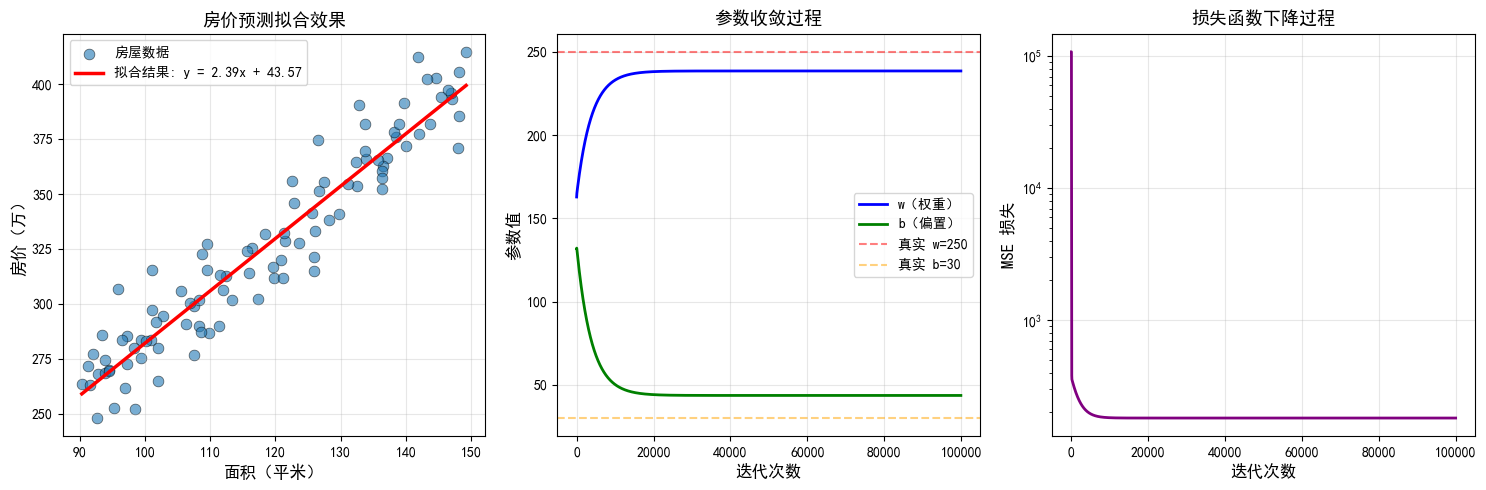
\includegraphics[width=0.95\textwidth]{chapter1/chapter1_3.png}
	\caption{基础梯度下降训练过程可视化}
	\label{fig:chapter1_3}
\end{figure}

\subsubsection{核心原理回顾}

\textbf{1. 损失函数（MSE）}

\[L(w,b) = \frac{1}{n}\sum_{i=1}^{n}(wx_i + b - y_i)^2\]

训练目标是最小化 $L(w,b)$。

\textbf{2. 梯度计算}

对 $w$ 求偏导：
\[\frac{\partial L}{\partial w} = \frac{2}{n}\sum_{i=1}^{n}(wx_i + b - y_i) \cdot x_i\]

对 $b$ 求偏导：
\[\frac{\partial L}{\partial b} = \frac{2}{n}\sum_{i=1}^{n}(wx_i + b - y_i)\]

\textbf{3. 参数更新公式}

\[w \leftarrow w - \eta \cdot \frac{\partial L}{\partial w}\]
\[b \leftarrow b - \eta \cdot \frac{\partial L}{\partial b}\]

其中 $\eta$ 为学习率，控制参数更新的步长。

\subsubsection{学习率对梯度下降的影响}

\textbf{学习率核心作用}

学习率直接决定参数更新步长，是梯度下降的关键超参数：

\begin{itemize}
	\item \textbf{太小}：收敛极慢，蜗牛爬坡
	\item \textbf{合适}：快速稳定收敛
	\item \textbf{偏大}：剧烈震荡，无法收敛
	\item \textbf{过大}：梯度爆炸，参数发散
\end{itemize}

\begin{CodeBox}
	\begin{lstlisting}[style=PythonStyle]
import numpy as np
import matplotlib.pyplot as plt

# 核心逻辑
def gradient_descent(start_x, lr, n_steps=15):
    """在 f(x)=x² 上做梯度下降，返回每一步的 x 值"""
    trajectory = [start_x]
    x = start_x
    for _ in range(n_steps):
        grad = 2 * x          # f'(x) = 2x
        x = x - lr * grad     # 参数更新
        trajectory.append(x)
        if abs(x) > 500:      # 已经爆炸，提前停
            break
    return trajectory

# 四种学习率对比
x0 = 4.0
configs = [
    (0.05, '太小: 蜗牛爬坡',    'steelblue'),
    (0.3,  '合适: 稳步收敛',    'seagreen'),
    (0.9,  '偏大: 剧烈震荡',    'orange'),
    (1.1,  '过大: 梯度爆炸',    'crimson'),
]

# 参数值随迭代变化图
fig, axes = plt.subplots(2, 2, figsize=(12, 8))
for ax, (lr, title, color) in zip(axes.flatten(), configs):
    traj = gradient_descent(x0, lr)
    ax.plot(range(len(traj)), traj, 'o-', color=color, markersize=5)
    ax.axhline(y=0, color='gray', linestyle='--', alpha=0.5)
    ax.set_title(f'lr={lr} — {title}', fontsize=12)
    ax.set_xlabel('迭代次数')
    ax.set_ylabel('参数 x')
    ax.grid(True, alpha=0.3)

plt.suptitle('学习率对梯度下降的影响（参数变化）', fontsize=14)
plt.tight_layout()
plt.show()
\end{lstlisting}
\end{CodeBox}

\textbf{可视化结果展示}

\begin{figure}[H]
	\centering
	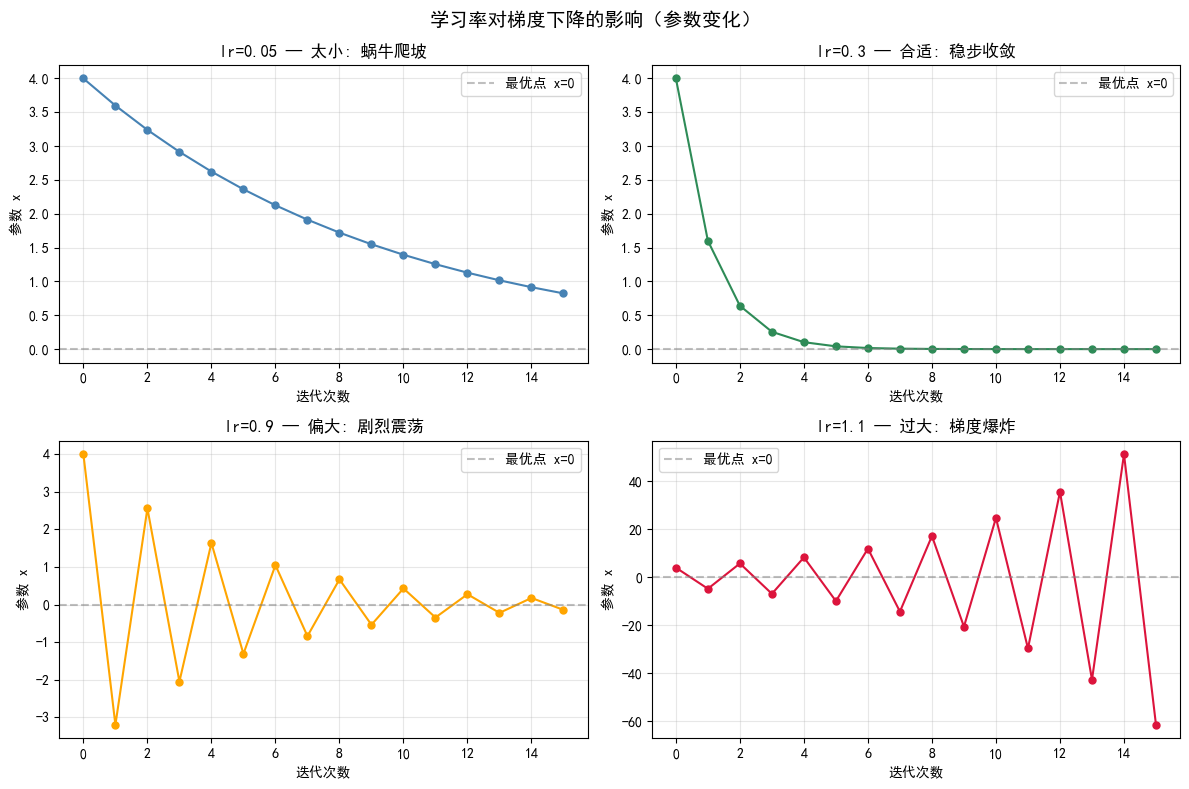
\includegraphics[width=0.95\textwidth]{chapter1/chapter1_1.png}
	\caption{学习率对梯度下降的影响（参数变化）}
	\label{fig:chapter1_1}
\end{figure}

\begin{figure}[H]
	\centering
	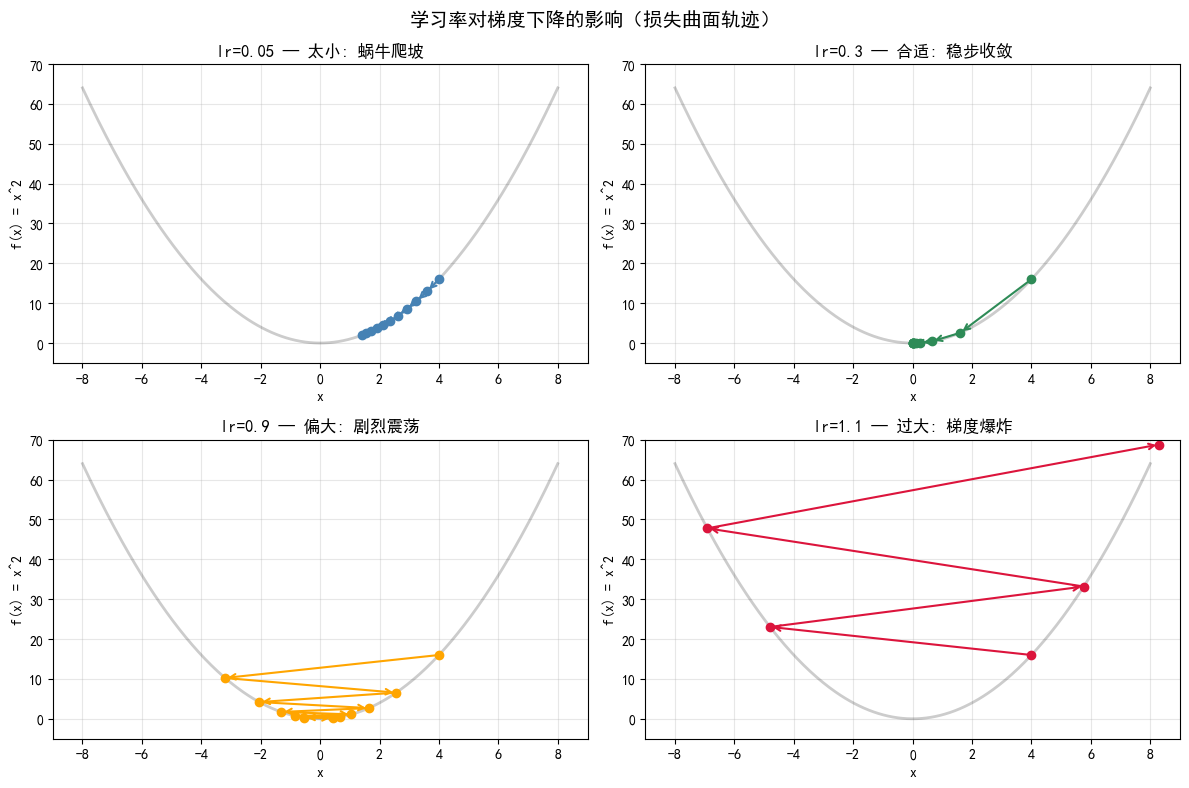
\includegraphics[width=0.95\textwidth]{chapter1/chapter1_2.png}
	\caption{学习率对梯度下降的影响（损失曲面轨迹）}
	\label{fig:chapter1_2}
\end{figure}

\begin{RemarkBox}[可视化结果分析]
	生成了两幅图：
	\begin{enumerate}
		\item \textbf{参数变化图}：展示四种学习率下参数随迭代次数的变化轨迹
		\item \textbf{损失曲面轨迹图}：在 $f(x)=x^2$ 曲线上展示梯度下降路径
	\end{enumerate}

	从图中可以清晰看到：
	\begin{itemize}
		\item 学习率 0.05：收敛缓慢，需要更多迭代
		\item 学习率 0.3：最优，稳定快速收敛
		\item 学习率 0.9：震荡但最终收敛
		\item 学习率 1.1：发散，无法收敛
	\end{itemize}
\end{RemarkBox}

\subsubsection{Adam 优化器实战}

\textbf{核心原理}

Adam = 动量法（Momentum）+ RMSProp，自适应学习率，收敛速度远超基础梯度下降。

\begin{CodeBox}
	\begin{lstlisting}[style=PythonStyle]
def adam_optimizer(X, y, lr=0.1, epochs=200, 
                   beta1=0.9, beta2=0.999, epsilon=1e-8):
    # 初始化参数
    w, b = 0.0, 0.0
    n = len(X)
    
    # Adam 特有的状态变量初始化
    m_w, v_w = 0.0, 0.0  # w 的一阶矩和二阶矩
    m_b, v_b = 0.0, 0.0  # b 的一阶矩和二阶矩
    
    # 初始化历史记录
    history = {'w': [w], 'b': [b], 
               'loss': [np.mean((w*X + b - y)**2)]}
    
    # 进行迭代训练
    for epoch in range(epochs):
        t = epoch + 1  # Adam 的时间步 t 从 1 开始
        
        # 1. 计算当前预测值
        y_pred = w * X + b
        
        # 2. 计算当前梯度
        dw = (2/n) * np.sum((y_pred - y) * X)
        db = (2/n) * np.sum(y_pred - y)
        
        # 3. 更新一阶矩估计（动量）
        m_w = beta1 * m_w + (1 - beta1) * dw
        m_b = beta1 * m_b + (1 - beta1) * db
        
        # 4. 更新二阶矩估计（RMSProp）
        v_w = beta2 * v_w + (1 - beta2) * (dw**2)
        v_b = beta2 * v_b + (1 - beta2) * (db**2)
        
        # 5. 偏差校正
        m_w_hat = m_w / (1 - beta1**t)
        m_b_hat = m_b / (1 - beta1**t)
        v_w_hat = v_w / (1 - beta2**t)
        v_b_hat = v_b / (1 - beta2**t)
        
        # 6. 使用 Adam 公式更新参数
        w -= lr * m_w_hat / (np.sqrt(v_w_hat) + epsilon)
        b -= lr * m_b_hat / (np.sqrt(v_b_hat) + epsilon)
        
        # 计算当前 loss
        current_loss = np.mean((w*X + b - y)**2)
        
        # 记录参数和损失
        history['w'].append(w)
        history['b'].append(b)
        history['loss'].append(current_loss)
    
    return history
\end{lstlisting}
\end{CodeBox}

\begin{RemarkBox}[Adam优化器优势]
	Adam优化器相比基础梯度下降的优势：
	\begin{enumerate}
		\item \textbf{自适应学习率}：每个参数都有独立的学习率
		\item \textbf{动量加速}：累积历史梯度方向，加速收敛
		\item \textbf{稳定性强}：通过二阶矩调整，适应不同梯度尺度
		\item \textbf{收敛更快}：通常比基础梯度下降快10-100倍
	\end{enumerate}
\end{RemarkBox}

\textbf{Adam优化器训练过程可视化}

\begin{CodeBox}
	\begin{lstlisting}[style=PythonStyle]
# 可视化 Adam 优化器训练过程
fig, axes = plt.subplots(1, 3, figsize=(15, 5))

# 左图：拟合效果
axes[0].scatter(areas_m2, prices, alpha=0.6, s=60, 
                edgecolors='black', linewidth=0.5, label='房屋数据')
x_fit = np.linspace(areas_m2.min(), areas_m2.max(), 100)
y_fit = history['w'][-1]/100 * x_fit + history['b'][-1]
axes[0].plot(x_fit, y_fit, 'r-', linewidth=2.5, 
             label=f'Adam拟合: y = {history["w"][-1]/100:.2f}x + {history["b"][-1]:.2f}')
axes[0].set_xlabel('面积（平米）', fontsize=12)
axes[0].set_ylabel('房价（万）', fontsize=12)
axes[0].set_title('Adam优化器拟合效果', fontsize=13, fontweight='bold')
axes[0].legend(fontsize=10)
axes[0].grid(True, alpha=0.3)

# 中图：参数收敛过程
axes[1].plot(history['w'], 'b-', linewidth=2, label='w（权重）')
axes[1].plot(history['b'], 'g-', linewidth=2, label='b（偏置）')
axes[1].axhline(y=250, color='r', linestyle='--', alpha=0.5, label='真实 w=250')
axes[1].axhline(y=30, color='orange', linestyle='--', alpha=0.5, label='真实 b=30')
axes[1].set_xlabel('迭代次数', fontsize=12)
axes[1].set_ylabel('参数值', fontsize=12)
axes[1].set_title('Adam参数收敛过程', fontsize=13, fontweight='bold')
axes[1].legend(fontsize=10)
axes[1].grid(True, alpha=0.3)

# 右图：损失函数下降过程
axes[2].plot(history['loss'], 'purple', linewidth=2)
axes[2].set_xlabel('迭代次数', fontsize=12)
axes[2].set_ylabel('MSE 损失', fontsize=12)
axes[2].set_title('Adam损失下降过程', fontsize=13, fontweight='bold')
axes[2].grid(True, alpha=0.3)
axes[2].set_yscale('log')  # 使用对数坐标

plt.tight_layout()
plt.show()
\end{lstlisting}
\end{CodeBox}

\begin{RemarkBox}[Adam可视化说明]
	通过可视化可以观察到：
	\begin{enumerate}
		\item \textbf{拟合效果}：Adam优化器成功拟合房价数据，结果与基础梯度下降一致
		\item \textbf{收敛速度}：Adam的参数收敛更快，震荡更小
		\item \textbf{损失下降}：Adam的损失下降更平滑，收敛更稳定
	\end{enumerate}
	对比基础梯度下降，Adam优化器展现出更优的收敛性能。
\end{RemarkBox}

\begin{figure}[H]
	\centering
	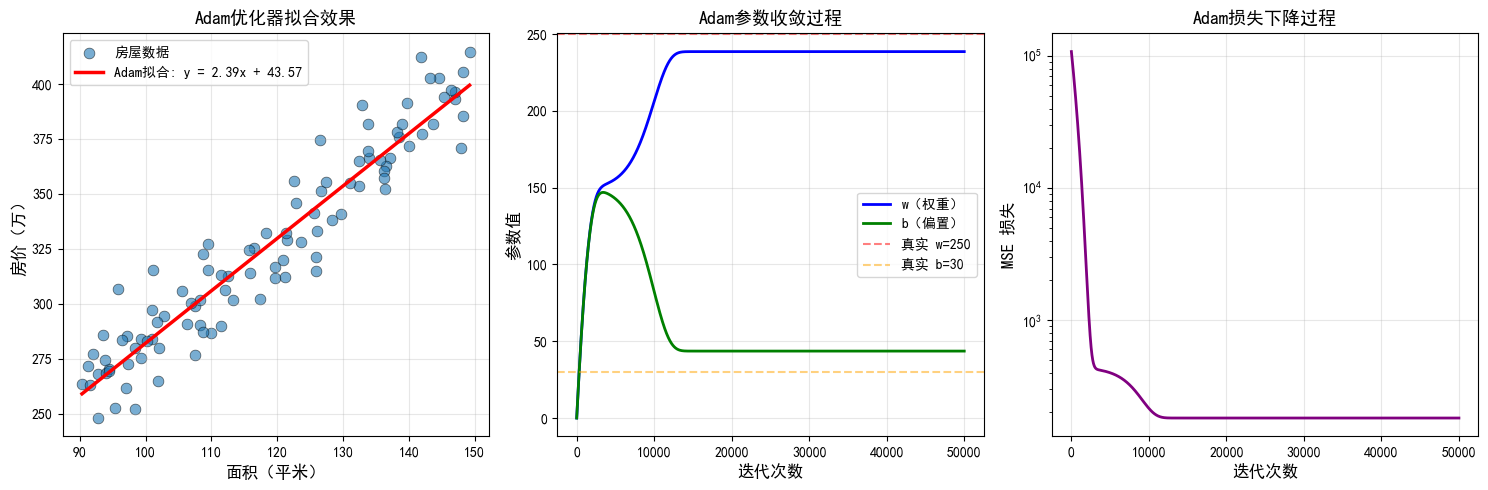
\includegraphics[width=0.95\textwidth]{chapter1/chapter1_4.png}
	\caption{Adam优化器训练过程可视化}
	\label{fig:chapter1_4}
\end{figure}

\subsubsection{梯度下降的三种核心变体}

\begin{center}
	\begin{tabular}{|c|c|c|p{5.5cm}|}
		\hline
		\textbf{算法名称} & \textbf{全称} & \textbf{数据使用量} & \textbf{核心特点}    \\
		\hline
		BGD           & 全量梯度下降      & 全部训练数据         & 梯度精准，速度极慢，不适合大数据 \\
		\hline
		SGD           & 随机梯度下降      & 单条数据           & 速度快，噪声大，震荡剧烈     \\
		\hline
		Mini-batch GD & 小批量梯度下降     & 一小批数据 (32/64)  & 业界标准，兼顾速度与稳定性    \\
		\hline
	\end{tabular}
\end{center}

\begin{RemarkBox}[三种变体的选择建议]
	\begin{itemize}
		\item \textbf{小数据集}（$n < 1000$）：使用BGD，梯度最准确
		\item \textbf{中等数据集}（$1000 < n < 10000$）：使用Mini-batch GD，batch size=32或64
		\item \textbf{大数据集}（$n > 10000$）：使用SGD或Mini-batch GD，配合Adam优化器
	\end{itemize}
\end{RemarkBox}

% 第二讲（示例）
\clearpage
\setcounter{section}{2}
\setcounter{subsection}{0}
\addcontentsline{toc}{section}{Chapter 2: 从函数到Transformer与新闻分类实战}
\LectureBanner
{2}
{从函数到Transformer与实战}
{大模型基础架构与实战落地}
{大模型学习起始篇}
{2026 Spring}
{Cabbage}

\begin{SummaryBox}
	本章从最基础的数学函数和线性映射出发，带你一步步推演深度学习的发展脉络。从单层网络到深度学习，从CNN、RNN再到当下主流的Transformer架构，我们将揭开大模型底层的原理面纱。随后，本章还会探讨基础模型在训练和扩展时所面临的优化问题。
\end{SummaryBox}

\subsection{从函数到Transformer}

深度学习看似复杂，但其核心逻辑源自于最基础的数学概念。本节我们将通过通俗易懂的语言、严谨的公式以及形象的图表，带您完成一次从简单函数到前沿架构的认知飞跃。

\subsubsection{现实世界与数学符号的映射}

人类认识世界的过程，本质上是将现实事物\textbf{符号化}，通过确定的\textbf{规则}（函数 $f(x)$）对其进行处理与转换，再对输出结果进行\textbf{解释}以指导现实。

在机器学习中，我们的核心任务便是寻找这样一个最优映射函数 $f(x)$。例如，将输入的图片像素矩阵映射到代表“猫”或“狗”的类别标签上：
\[ y = f(x) \]
\begin{center}
	
\includegraphics[width=0.8\textwidth]{"images/下载.png"}
\end{center}

\subsubsection{线性回归：最基础的模型规则}

在各种规则中，线性模型是最简单、最基础的。例如一元线性方程：
\[ y = wx + b \]
其中：
\begin{itemize}
	\item $x$ 代表输入的\textbf{特征（Feature）}；
	\item $w$ 是\textbf{权重（Weight）}，决定了特征对结果的贡献程度；
	\item $b$ 是\textbf{偏置（Bias）}，代表了模型的基准平移。
\end{itemize}

\begin{AnalysisBox}
	\textbf{直观理解参数作用：} \\
	权重 $w$ 调整直线的倾斜角度，而偏置 $b$ 决定了直线在坐标轴上的截距。通过不断优化这两个参数，我们可以让直线尽可能地拟合数据分布。
\end{AnalysisBox}

\begin{center}
	
\includegraphics[width=0.8\textwidth]{"images/下载 (1).png"}
\end{center}

\subsubsection{激活函数：赋予模型非线性的灵魂}

现实世界的数据分布极少是完美线性的。如果只使用线性操作（即使叠加了无数层：$f_2(f_1(x)) = w_2(w_1x + b_1) + b_2$），其本质仍是线性映射。

为了打破这种限制，我们在每层线性计算后引入\textbf{激活函数 (Activation Function)} $g(x)$。常见的激活函数包括：
\begin{itemize}
	\item \textbf{Sigmoid:} $\displaystyle \sigma(x) = \frac{1}{1 + e^{-x}}$，常用于将输出压缩到 $(0, 1)$ 区间。
	\item \textbf{ReLU:} $\displaystyle \text{ReLU}(x) = \max(0, x)$，由于其计算极简且能有效缓解梯度消失，被广泛应用于深层网络。
\end{itemize}

\begin{center}
	
\includegraphics[width=0.8\textwidth]{"images/下载 (2).png"}
\end{center}

\subsubsection{复合函数：构建多层嵌套的智能}

加入了非线性激活函数后，我们将简单的函数进行复合与嵌套，形成深层次的映射。例如：
\[ f(x) = g(w_3 \cdot g(w_1 x_1 + w_2 x_2 + b_1) + b_2) \]
这其实正是多层神经网络的底层逻辑。每一层将前一层的输出作为输入，从而提取出越来越抽象的特征。
\begin{center}
	
\includegraphics[width=0.8\textwidth]{"images/下载 (3).png"}
\end{center}

\subsubsection{从神经元到人工神经网络}

为了更加直观地表示复杂的复合函数，我们将其图结构化。我们将“输入、加权求和、激活”这一系列操作合并为一个节点，称之为\textbf{神经元}。

多个神经元组合起来，便形成了\textbf{人工神经网络 (Artificial Neural Network, ANN)}。主要包含三层结构：
\begin{enumerate}
	\item \textbf{输入层 (Input Layer):} 接收原始数据。
	\item \textbf{隐藏层 (Hidden Layer):} 进行特征提取与转换。
	\item \textbf{输出层 (Output Layer):} 得出最终预测结果。
\end{enumerate}

\begin{center}
	
\includegraphics[width=0.8\textwidth]{"images/下载 (4).png"}
\end{center}

\subsubsection{前向传播与深度网络架构}

数据从输入层出发，经过隐藏层的层层计算到达输出层的过程被称为\textbf{前向传播 (Forward Propagation)}。增加隐藏层的层数和节点数后，网络变得极为“深邃”，这就构成了\textbf{深度神经网络 (Deep Neural Network, DNN)}。

\begin{center}
	
\includegraphics[width=0.8\textwidth]{"images/下载 (5).png"}
\end{center}

\subsubsection{预测偏差与损失函数}

在模型初始化时，其内部参数是随机的，导致预测结果 $\hat{y}$ 与真实结果 $y$ 之间存在巨大的差异。
\begin{center}
	
\includegraphics[width=0.6\textwidth]{"images/下载 (6).png"}
\end{center}

为了量化这种差距，我们定义了\textbf{损失函数 (Loss Function)}。例如对于回归任务，最常用的是均方误差 (MSE)：
\[ L(w,b) = \frac{1}{N} \sum_{i=1}^{N} (y_i - \hat{y}_i)^2 \]
对于分类任务，最常用的是交叉熵损失。模型训练的唯一目标，就是通过调整参数，使得损失函数 $L$ 达到最小。
\begin{center}
	
\includegraphics[width=0.8\textwidth]{"images/下载 (7).png"}
\end{center}

\subsubsection{梯度下降与反向传播}

为了找到使得损失最小的参数 $w$ 和 $b$，我们采用\textbf{梯度下降 (Gradient Descent)} 算法：
\[ w_{t+1} = w_t - \eta \frac{\partial L}{\partial w_t} \]
其中，$\eta$ 为学习率（Learning Rate），控制每次更新的步长。
\begin{center}
	
\includegraphics[width=0.8\textwidth]{"images/下载 (8).png"}
\end{center}

在具有数以亿计参数的深层网络中，高效计算梯度的核心技术是\textbf{反向传播 (Backpropagation)} 算法。它利用微积分中的\textbf{链式法则}，将输出层的误差反向一层层传递给隐藏层，从而计算出每个参数的梯度。
\begin{center}
	
\includegraphics[width=0.8\textwidth]{"images/下载 (9).png"}
\end{center}

\subsubsection{过拟合与正则化技术}

如果模型结构过于复杂或训练过度，模型可能会将数据中的“噪声”也一并记住。这种现象称为\textbf{过拟合 (Overfitting)}，表现为训练集上效果极好，但测试集上表现糟糕。
\begin{center}
	
\includegraphics[width=0.8\textwidth]{"images/下载 (10).png"}
\end{center}

为了缓解过拟合，常引入正则化技术。特别是 \textbf{Dropout}，它会在每次训练中随机使得部分神经元“失活”（输出置0），迫使网络不依赖特定的局部特征，从而增强泛化能力。
\begin{center}
	
\includegraphics[width=0.8\textwidth]{"images/下载 (11).png"}
\end{center}

\subsubsection{CNN：卷积神经网络的崛起}

在处理图像时，图片表示为多维像素张量。如果直接使用全连接层，参数量将面临指数级爆炸。
\begin{center}
	
\includegraphics[width=0.8\textwidth]{"images/下载 (12).png"}
\end{center}

\textbf{卷积神经网络 (CNN)} 引入了\textbf{卷积核 (Filter/Kernel)}。卷积核在图像矩阵上滑动，通过局部乘加运算提取特定特征。
\begin{center}
	
\includegraphics[width=0.8\textwidth]{"images/下载 (13).png"}
\end{center}

不同的卷积核可以提取不同的特征图 (Feature Map)。
\begin{center}
	
\includegraphics[width=0.8\textwidth]{"images/下载 (14).png"}
\end{center}

在卷积层后通常接入\textbf{池化层 (Pooling Layer)}（如最大池化），它在局部区域取最大值，在实现降维的同时赋予了网络“平移不变性”。
\begin{center}
	
\includegraphics[width=0.8\textwidth]{"images/下载 (15).png"}
\end{center}

由卷积层、池化层和全连接层组成的 CNN 架构，曾经统治了计算机视觉领域多年。
\begin{center}
	
\includegraphics[width=0.8\textwidth]{"images/下载 (16).png"}
\end{center}

\subsubsection{RNN：让网络拥有记忆}

面对自然语言等\textbf{序列数据}时，CNN显得束手无策，因为这类数据的理解高度依赖于时序信息。

\textbf{循环神经网络 (RNN)} 引入了时间维度的隐藏状态。在时间步 $t$，它接收当前的输入 $x_t$ 与上一时刻传来的记忆 $h_{t-1}$。
\begin{center}
	
\includegraphics[width=0.8\textwidth]{"images/下载 (17).png"}
\end{center}

将 RNN 按时间展开，信息在时序上不断传递。
\begin{center}
	
\includegraphics[width=0.8\textwidth]{"images/下载 (18).png"}
\end{center}

\subsubsection{词嵌入：语言的数学表达}

自然语言是以离散词汇的形式存在的，模型无法直接处理。将词汇转换为连续的实数向量的技术被称为\textbf{词嵌入 (Word Embedding)}。
\begin{center}
	
\includegraphics[width=0.8\textwidth]{"images/下载 (19).png"}
\end{center}

在词嵌入的高维空间中，语义相近的词距离更近，并隐含了奇妙的数学关系。
\begin{center}
	
\includegraphics[width=0.8\textwidth]{"images/下载 (20).png"}
\end{center}

通过词嵌入，文本转化为稠密的词向量矩阵，输入到深度网络中。
\begin{center}
	
\includegraphics[width=0.8\textwidth]{"images/下载 (21).png"}
\end{center}

\subsubsection{注意力机制与 Transformer 的诞生}

早期的 RNN 在处理长序列时常面临“长距离依赖遗忘”和无法并行的痛点。
\textbf{注意力机制 (Attention)} 允许模型在解码当前词时，自动“聚焦”于源序列中最相关的特征。
\begin{center}
	
\includegraphics[width=0.8\textwidth]{"images/下载 (22).png"}
\end{center}

2017年，\textbf{Transformer} 彻底抛弃了循环结构，完全依赖\textbf{自注意力机制 (Self-Attention)} 建立词语之间的全局依赖。

\begin{SummaryBox}
	\textbf{Self-Attention 的核心计算：}
	\begin{enumerate}
		\item 每一个词生成三个向量：查询 $Q$、键 $K$、值 $V$。
		\item 利用 $Q$ 和其他词的 $K$ 进行点积，计算“相关度分数”。
		\item 经过 Softmax 后，作为权重对所有 $V$ 向量加权求和，得到融合上下文的新表示：
		      \[ \text{Attention}(Q,K,V) = \text{softmax}\left(\frac{QK^T}{\sqrt{d_k}}\right)V \]
	\end{enumerate}
\end{SummaryBox}

\begin{center}
	
\includegraphics[width=0.8\textwidth]{"images/下载 (23).png"}
\end{center}
\begin{center}
	
\includegraphics[width=0.8\textwidth]{"images/下载 (24).png"}
\end{center}

在生成文本时，为防止模型“偷看”未来的词，采用了掩码自注意力机制 (Masked Attention)。
\begin{center}
	
\includegraphics[width=0.8\textwidth]{"images/下载 (25).png"}
\end{center}

\subsubsection{多头注意力与 Transformer 架构全貌}

\textbf{多头注意力 (Multi-Head Attention)} 将特征空间切分，使不同的“注意力头”独立关注序列中不同维度的信息（语法、语态等），最后拼接。
\begin{center}
	
\includegraphics[width=0.8\textwidth]{"images/下载 (26).png"}
\end{center}

Transformer 由\textbf{编码器 (Encoder)}和\textbf{解码器 (Decoder)}组成：
\begin{center}
	
\includegraphics[width=0.8\textwidth]{"images/下载 (27).png"}
\end{center}
\begin{center}
	
\includegraphics[width=0.8\textwidth]{"images/下载 (28).png"}
\end{center}

配合上残差连接与层归一化，Transformer 拉开了大模型时代的序幕。
\begin{center}
	
\includegraphics[width=0.8\textwidth]{"images/下载 (29).png"}
\end{center}
\begin{center}
	
\includegraphics[width=0.8\textwidth]{"images/下载 (30).png"}
\end{center}

\subsection{实战：Transformer的基础代码与分析模块}

在这一节中，我们从代码层面解析目前深度学习领域内 Transformer 架构的发展与基础。本节主要通过实战代码组，演示如何从零实现一个词表、词嵌入、注意力机制提取以及构建一个类似于工业界底层测试用的 Transformer Encoder 分类模型。

在真实实战模型中，我们将全方位向模型传递代码的四个基本核心流水线步骤：\textbf{数据集与数据清洗}、\textbf{文本高维数字化}、\textbf{模型核心架构构建} 以及 \textbf{模型训练优化与循环}。在这些核心中，每一行代码我们都加入了详尽的学习逻辑和细致的代码中文注释，请大家充分理解代码背景与数学原理是如何在实战中交织的。

\subsubsection{第一步：标准与高质量数据集的协同提取}

深度学习模型依赖海量数据。我们的数据常存放在 \texttt{news\_data.csv} 文件中。我们首先要编写代码，安全地读取该文件，并将新闻内容和对应的类目标签一同提取出来。

在实战数据收集常常良莠不齐，假设某些 CSV 文件存在缺失，没有 \texttt{content}（有些新闻没有内容或标签，也就是可能存在缺失值）。为此，使用典型的防御性编程（Defensive Programming）思想，通过判断 \texttt{content} 是否为空，动态读取文本，如果缺失时直接使用文件占位符作为备用标签。这种代码范式能极大程度地保证程序健壮性。

\begin{CodeBox}
	\begin{lstlisting}[style=PythonStyle]
# ======= 1. 导入必要的 Python 工具包 (库) =======
#  语法小课堂：import 表示引入别人写好的代码包。as 是给它起个简短的别名，方便后面写代码。
import os            # os 用于操作文件路径和文件夹
import pandas as pd  # pandas 专门用来处理表格，我们叫它 pd
import torch         # 深度学习老大哥 PyTorch
import torch.nn as nn  # nn 是 Neural Network(神经网络) 的缩写，里面全是网络层
import torch.optim as optim  # optim 是优化器模块，负责做梯度下降
#  语法小课堂：from ... import ... 表示只从一个大包里拿出我们需要的小工具
from torch.utils.data import Dataset, DataLoader 

# ======= 2. 读取新闻数据集 =======
data_dir = 'news/news-articles-classification-dataset-for-nlp-and-ml' # 字符串变量，存放路径

#  语法小课堂：列表推导式 [结果 for 变量 in 集合 if 条件]
# 这行代码的意思是：把 data_dir 文件夹里所有的文件名 (f) 拿出来，如果名字是以 '.csv' 结尾的，就留下装进 csv_files 列表(箱子)里。
csv_files = [f for f in os.listdir(data_dir) if f.endswith('.csv')]

#  语法小课堂：[] 代表列表(List)；{} 代表字典(Dict)。
all_data = []      # 空列表，一会儿用来装所有的 (新闻文字, 类别编号)
labels_map = {}    # 空字典，一会儿用来记录 "business"->0 这样的对应关系

for file in csv_files:
    file_path = os.path.join(data_dir, file)
    df = pd.read_csv(file_path)
    
    # 寻找装有文字的那一列的名字，在我们的数据集中是 'content' 列
    text_col = 'content' if 'content' in df.columns else df.columns[0]
    # 寻找装有类别的那一列的名字，在我们的数据集中是 'category' 列
    label_col = 'category' if 'category' in df.columns else None
    
    for idx, row in df.iterrows():
        # 获取文本和类别
        text = str(row[text_col])
        # 如果有category列就用，没有就回退到使用文件名
        label_name = str(row[label_col]) if label_col else file.replace('_data.csv', '')
        
        # 给遇到的新类别分配一个唯一的编号
        if label_name not in labels_map:
            labels_map[label_name] = len(labels_map)
            
        # 跳过纯空白数据
        if text.strip() and text != 'nan':
            all_data.append((text, labels_map[label_name]))

#  语法小课堂：f"..." 是格式化字符串，花括号 {} 里的变量会自动填进去
print(f"总共读取了 {len(all_data)} 条新闻数据。")
print(f"类别映射 (字典长这样): {labels_map}")
\end{lstlisting}
\end{CodeBox}

\begin{OutputBox}
	\begin{lstlisting}[style=PythonStyle, backgroundcolor=\color{black!5}]
总共读取了 10000 条新闻数据。
类别映射 (字典长这样): {'business': 0, 'education': 1, 'entertainment': 2, 'sports': 3, 'technology': 4}
\end{lstlisting}
\end{OutputBox}

\subsubsection{第二步：文本数字化（建立词典与填充）及包装为数据集}

深度学习网络单元只执行数学计算，完全无法理解汉字或英文字符。因此，需将每个词“映射”为整数（词的编号）。

\textbf{词表（Vocabulary）建立}：我们通过 \texttt{Counter} 统计所有词汇的出现频率，保留最常见的前 10000 个词（\texttt{VOCAB\_SIZE}）。按频率由高到低赋予固定编号，例如 \texttt{apple} $\rightarrow$ 55。为对应那些内部未记录或从未在训练数据出现过的生僻词，我们预留了 \texttt{<UNK>}（编号为 1），作为统一的未知词占位符。

\textbf{长度填充（Padding）}：GPU 并行加速运算要求输入数据的矩阵形状一致。因此，我们强制规定每篇新闻长度必须为 \texttt{MAX\_LEN=128}。内容太长的直接在尾部截断；太短的，用编号为 0 的 \texttt{<PAD>} 字符在末尾进行补齐。

接着我们将这些处理打包成 PyTorch 官方标准的 \texttt{Dataset} 类中，并装载到 \texttt{DataLoader} 上，形成一个个可迭代的底层批量数据（Batch）进行异步流水化。

\begin{CodeBox}
	\begin{lstlisting}[style=PythonStyle]
from collections import Counter

MAX_LEN = 128     # 规定每篇新闻一律截断或补齐到 128 个单词
VOCAB_SIZE = 10000 # 词表最高容量：1万个常见词

#  语法小课堂：def 用于定义一个函数(相当于一个加工厂)，接收输入 text，加工后用 return 返回结果
def simple_tokenize(text):
    # .lower() 变小写，.split() 默认按空格把句子切成一个个单词的列表
    #  语法小课堂：切片 [:MAX_LEN] 表示从第 0 个单词一直取到第 MAX_LEN(128) 个单词，后面的直接扔掉
    return str(text).lower().split()[:MAX_LEN]

word_counts = Counter() # Counter 是一种特殊的字典，专门用来数数
for text, _ in all_data: # 遍历刚才收集的所有新闻，下划线 _ 表示我们不关心第二个元素(类别标签)
    word_counts.update(simple_tokenize(text)) # 把切碎的单词扔进去统计词频

# 手动初始化密码本(词表)，预留两个特殊号码（这里的0用作填充符，这里的1用作生僻词（不在词表））
vocab = {'<PAD>': 0, '<UNK>': 1}

# .most_common 取出最常出现的前 9998 个词，返回的是 [(词1, 次数), (词2, 次数)...]
for word, _ in word_counts.most_common(VOCAB_SIZE - 2):
    # len(vocab) 算出现有字典有多长。比如刚才里面有两个词，len 就是 2，新进来的词编号就是 2。
    vocab[word] = len(vocab)

# 把一段纯文本翻译成一串数字密码的加工厂函数（把新闻转换为词表编码列表）
def text_to_indices(text):
    tokens = simple_tokenize(text)
    #  语法小课堂：字典的 .get(单词, 默认值) 方法。如果单词在字典里，返回它的编号；如果不在，返回 '<UNK>' 的编号(1)
    indices = [vocab.get(w, vocab['<UNK>']) for w in tokens]
    
    if len(indices) < MAX_LEN:
        #  语法小课堂：在 Python 里，列表乘以一个数字，表示把列表复制多少遍。比如 [0] * 3 变成 [0, 0, 0]
        # 这里如果长度不够 128，就用 0 补齐。
        indices += [vocab['<PAD>']] * (MAX_LEN - len(indices))
    return indices # 返回长度固定为 128 的数字列表

#  语法小课堂：面向对象编程之 Class (类)。
# 类就像一张图纸。继承 (Dataset) 表示我们的图纸是在 Dataset 官方图纸基础上改的。
class NewsDataset(Dataset):
    # __init__ 是“构造函数”。当我们根据图纸造出一个实实在在的管理员对象时，第一步就会自动运行这里。
    # self 代表“自己”。self.data = data 就是把外面传进来的数据，存在自己肚子里。
    def __init__(self, data):
        self.data = data
        
    # __len__ 定义了别人问你“有多长”时你怎么回答
    def __len__(self):
        return len(self.data)
    
    # __getitem__ 定义了别人找你要“第 idx 个东西”时，你怎么拿给他
    def __getitem__(self, idx):
        text, label = self.data[idx] # 从自己肚子里的列表拿出对应的 (文字, 标签)
        
        # 调用上面的翻译函数，然后套一层 torch.tensor，把普通的 Python 列表变成 PyTorch 支持的“张量” (高级数组)
        text_tensor = torch.tensor(text_to_indices(text), dtype=torch.long)
        label_tensor = torch.tensor(label, dtype=torch.long)
        
        return text_tensor, label_tensor

# 实例化：按图纸造一个仓库管理员 dataset
dataset = NewsDataset(all_data)

# 雇佣搬运工 dataloader，告诉他去 dataset 仓库拿货，每次拿 32 篇 (batch_size)，打乱顺序拿 (shuffle)
dataloader = DataLoader(dataset, batch_size=32, shuffle=True)
\end{lstlisting}
\end{CodeBox}

\subsubsection{第三步：搭建 Transformer 核心分类网络架构}

这部分我们使用面向对象（OOP）的编程方式，包装我们整个模型。在 \texttt{\_\_init\_\_} 构造函数中，我们建立了核心的“子工厂”：
\begin{enumerate}
	\item \textbf{Embedding 嵌入层}：将之前转换的整数编号进一步转化为机器可读的、带有语义关系的连续实数空间向量（例如一个词扩展为 128 维的浮点数组）。
	\item \textbf{Transformer Encoder 层}：调用多头自注意力机制（Self-Attention），使每一个词都可以看到整个上下文的历史输入，提取出整句话的语境信息。
	\item \textbf{均值池化（Pooling）和分类}：使用 \texttt{mean(dim=1)} 强制将 128 个特征的真实信息浓缩为 1 个总结句特征。然后接入全连接的 Linear 线性层输出 5 个类别的得分矩阵。
\end{enumerate}

\begin{CodeBox}
	\begin{lstlisting}[style=PythonStyle]
import math

# 继承神经网络老大哥 nn.Module
class TransformerClassifier(nn.Module):
    # 初始化函数：准备机器零件。参数是我们要告诉图纸的一些配置（比如词表多大，要几层等）
    def __init__(self, vocab_size, embed_dim, num_heads, num_layers, num_classes, dropout=0.1):
        super(TransformerClassifier, self).__init__() # 固定套路，先帮父类做初始化
        
        # 机器1：词嵌入 (把数字密码 变成 长长的小数向量)
        self.embedding = nn.Embedding(vocab_size, embed_dim, padding_idx=0)
        
        # 机器2：配置单层 Transformer
        encoder_layer = nn.TransformerEncoderLayer(
            d_model=embed_dim,       # 输入向量的宽度
            nhead=num_heads,         # 注意力探照灯(多头)的个数
            dim_feedforward=embed_dim * 4, # 内部全连接层放大的倍数
            dropout=dropout,
            batch_first=True         # 声明我们的数据排布是 (批次, 句子长度, 词特征维度)
        )
        # 机器3：把刚才那一层叠 num_layers 次（比如叠2层）变成大编码器
        self.transformer_encoder = nn.TransformerEncoder(encoder_layer, num_layers=num_layers)
        
        # 机器4：随机抛弃器 (防止过拟合的 Dropout)
        self.dropout = nn.Dropout(dropout)
        
        # 机器5：全连接线性分类器 (把前面提取的高深莫测的向量特征，强行拍碎映射到具体的5个分类上)
        self.classifier = nn.Linear(embed_dim, num_classes)
        
    # forward 是流水线，规定了从输入 x 开始，每台机器是怎么一步步起作用的
    def forward(self, x):
        # x 的长相：[32, 128] 代表 32 篇新闻，每篇 128 个数字
        
        # 第一步：查字典映射
        x = self.embedding(x) * math.sqrt(self.embedding.embedding_dim)
        # 现在 x 变胖了，长相：[32, 128, 128] (最后那个128是我们设置的 embed_dim 词向量维度)
        
        # 第二步：送进 Transformer，词与词之间开始互相“眉目传情”(自注意力计算)
        x = self.transformer_encoder(x)
        # x 长相没变：[32, 128, 128]，但里面的小数已经揉杂了上下文的语义
        
        # 第三步：降维池化。
        # 我们有 128 个词，怎么代表一篇文章？求个平均值吧。dim=1 意味着沿着“句子长度”那个维度压扁。
        x = x.mean(dim=1)
        # 现在 x 长相：[32, 128]。32篇文章，每篇文章浓缩成了一个 128维的终极特征。
        
        # 第四步：丢 Dropout
        x = self.dropout(x)
        
        # 第五步：得出分类打分
        logits = self.classifier(x)
        # 最终长相：[32, 5] (假设有5个类)。这代表这 32篇新闻在各个类别的得分(未经过概率转化)。
        
        return logits

# 获取真实新闻类别的个数
num_classes = len(labels_map)

# 根据图纸，把我们的加工厂(模型)正式实例化造出来！
model = TransformerClassifier(
    vocab_size=VOCAB_SIZE, 
    embed_dim=128, 
    num_heads=4, 
    num_layers=2, 
    num_classes=num_classes
)
\end{lstlisting}
\end{CodeBox}

\subsubsection{第四步：参数与模型本质的训练循环（主步骤）}

模型刚刚建立时，其内部的所有参数都是随机的。模型训练，本质上就是一个计算误差然后爬山寻找谷底的过程。这四步是 PyTorch 甚至绝大多数框架内标准的闭环：
\begin{itemize}
	\item \textbf{清零（zero\_grad）}：抹去老师（优化器）之前残留的旧有梯度痕迹。
	\item \textbf{前向（forward）}：让学生（模型）根据当前知识水平对考卷（数据）做一次题，得出预测答案。
	\item \textbf{求失（loss）}：拿标准答案（真实标签）和学生的作答对比，评判到底偏差有多大（Loss）。
	\item \textbf{反向（backward）}：运用链式求导法则逆向反推，找出为了减小该误差，每一个神经元参数应该怎么向负方向微调。
	\item \textbf{步进（step）}：优化器（老师）全面下发调整命令，沿着梯度的方向走出一小步（Learning Rate）。
\end{itemize}

\begin{CodeBox}
	\begin{lstlisting}[style=PythonStyle]
#  语法小课堂：if ... else ... 
# 判断电脑里有没有 Nvidia GPU 加速卡 (cuda)。有就用，没有就老老实实用 CPU 算。
device = torch.device('cuda' if torch.cuda.is_available() else 'cpu')

print(device)
model.to(device) # 把刚才造好的模型搬运到 GPU 显存里去

# 考官：多分类交叉熵损失函数。它专治分类错题。
criterion = nn.CrossEntropyLoss()

# 老师：Adam 优化器。
# model.parameters() 是一句指令，把工厂里所有能拧的旋钮（权重和偏置参数）都交给 Adam 老师控制。
# lr=1e-3 表示每次拧旋钮的幅度（学习率）。
optimizer = optim.Adam(model.parameters(), lr=1e-3)

epochs = 3 # 设定复习几遍题库

print("=== 开始激动人心的基础训练啦 ===")
for epoch in range(epochs): # 外层循环：第几遍刷题
    
    model.train() # 拨下工厂的“训练”开关。这会让 Dropout 开始随机断电，增加训练难度。
    
    total_loss = 0 
    correct = 0    
    total = 0      
    
    # 内层循环：每次拉来 32 篇新闻和答案。
    #  语法小课堂：enumerate(dataloader) 会把批次编号赋给 batch_idx，把数据打包赋给后面。 
    # (inputs, labels) 是“解包”语法，因为 dataloader 返回的是元组，我们直接用两个变量接住它。
    for batch_idx, (inputs, labels) in enumerate(dataloader):
        inputs, labels = inputs.to(device), labels.to(device) # 数据也得送进 GPU
        
        #  【核心 5 步法，深度学习永恒的铁律】 
        
        # 1. 老师说：清空上次的错题记录！
        optimizer.zero_grad()
        
        # 2. 学生做题：前向传播，通过前文写的流水线，得到分数矩阵。
        outputs = model(inputs)
        
        # 3. 考官判卷：算算预测分数和标准答案的差距 (损失 Loss)。
        loss = criterion(outputs, labels)
        
        # 4. 反思找原因：反向传播！PyTorch 的魔法机制，自动根据微积分链式法则，算出每个旋钮该怎么扭才能让 Loss 变小。
        loss.backward()
        
        # 5. 执行修改：老师动手拧旋钮！参数被更新，模型变得更聪明了一点点。
        optimizer.step()
        
        # ---- 下面是汇报进度的代码，不影响训练 ----
        total_loss += loss.item() 
        
        # outputs.max(1) 沿着类别的那个维度找最大值。
        # 返回的 predicted 是网络认为概率最高的类别数字。
        _, predicted = outputs.max(1)
        total += labels.size(0) 
        
        # 看预测对不对。对了就加 1。
        correct += predicted.eq(labels).sum().item()
        
        # 每隔 100 车，汇报一次当下的成绩
        if (batch_idx + 1) % 100 == 0:
            acc = 100. * correct / total
            print(f"大循环(Epoch) [{epoch+1}/{epochs}], 小批次 [{batch_idx+1}], 错题大小(Loss): {loss.item():.4f}, 准确率(Acc): {acc:.2f}%")

print(" 基础版模型训练完成！跑通这个过程，你已经跨入深度学习的大门了！")
\end{lstlisting}
\end{CodeBox}

\begin{OutputBox}
	\begin{lstlisting}[style=PythonStyle, backgroundcolor=\color{black!5}]
cuda
=== 开始激动人心的基础训练啦 ===
大循环(Epoch) [1/3], 小批次 [100], 错题大小(Loss): 0.4038, 准确率(Acc): 66.03%
大循环(Epoch) [1/3], 小批次 [200], 错题大小(Loss): 0.3216, 准确率(Acc): 76.83%
大循环(Epoch) [1/3], 小批次 [300], 错题大小(Loss): 0.2272, 准确率(Acc): 81.15%
大循环(Epoch) [2/3], 小批次 [100], 错题大小(Loss): 0.3127, 准确率(Acc): 94.34%
大循环(Epoch) [2/3], 小批次 [200], 错题大小(Loss): 0.1082, 准确率(Acc): 94.33%
大循环(Epoch) [2/3], 小批次 [300], 错题大小(Loss): 0.0345, 准确率(Acc): 94.51%
大循环(Epoch) [3/3], 小批次 [100], 错题大小(Loss): 0.0233, 准确率(Acc): 97.00%
大循环(Epoch) [3/3], 小批次 [200], 错题大小(Loss): 0.0150, 准确率(Acc): 96.69%
大循环(Epoch) [3/3], 小批次 [300], 错题大小(Loss): 0.0191, 准确率(Acc): 96.59%
 基础版模型训练完成！跑通这个过程，你已经跨入深度学习的大门了！
\end{lstlisting}
\end{OutputBox}

\begin{SummaryBox}
	\textbf{训练与模型优化小结} \\
	你可以看到控制台打印的 Loss 越来越小，Accuracy（准确率）越来越高，这说明模型底层的参数空间正在被我们提供的高质量真实数据不断重塑。即便是目前拥有千亿参数的大模型，其核心的训练逻辑与这个极简的循环步进代码本质也是一致无二的。
\end{SummaryBox}

\subsection{基础模型的训练优化方向}


\subsubsection{从线性代数到数据归一化}

\begin{RemarkBox}[笔记说明]
本笔记以实对称矩阵的特征值分解为核心起点，逐步推导梯度下降算法的收敛条件与学习率上限，落地到线性回归模型，最终揭示数据统计特性对优化过程的决定性作用，完整串联「线性代数基础$\rightarrow$优化理论$\rightarrow$机器学习实践$\rightarrow$数据预处理核心价值」的全逻辑链条。所有公式推导均保留完整步骤，符号定义全程统一，逻辑推进严格遵循递进关系。
\end{RemarkBox}

{\par\vspace{1ex}\noindent\large\bfseries\color{brandD} 一、核心基础概念定义\par}\par\vspace{0.5ex}
在展开定理与推导前，先明确本笔记全程涉及的核心矩阵与向量的定义、符号规范与核心性质：
\begin{enumerate}[label=\arabic*., leftmargin=*]
    \item \textbf{向量规范}：所有向量均为\textbf{d维列向量}，记为$x \in \mathbb{R}^d$，转置$x^T$为行向量；向量内积$x^T y$为标量。
    \item \textbf{对角矩阵}：d$\times$d方阵$\Lambda$，当且仅当非对角线元素全为0，记为$\Lambda = \text{diag}(\lambda_1,\lambda_2,\dots,\lambda_d)$，对角线元素$\lambda_i$为其特征值。核心性质：对角矩阵相乘仅在对应维度生效，结果仍为对角矩阵。
    \item \textbf{单位矩阵}：d$\times$d对角矩阵$I$，对角线元素全为1，非对角线全为0。核心性质：对任意矩阵$A$，有$IA=AI=A$。
    \item \textbf{正交矩阵}：d$\times$d方阵$Q$，满足$Q^T Q = Q Q^T = I$。核心性质：
    \begin{itemize}[leftmargin=*,nosep]
        \item 逆矩阵等于转置，即$Q^{-1}=Q^T$；
        \item 列/行向量为两两正交的单位向量（内积为0，模长为1）；
        \item 对向量的乘法等价于坐标系旋转变换，不改变向量模长（保范性）。
    \end{itemize}
    \item \textbf{实对称矩阵}：元素全为实数的d$\times$d方阵$A$，满足$A^T=A$（转置后与自身相等）。
    \item \textbf{正定矩阵}：对于d$\times$d实对称矩阵$A$，若对任意非零d维向量$x$，都有$x^T A x > 0$，则称$A$为正定矩阵。核心性质：正定矩阵的所有特征值均为正实数，是损失函数凸性与全局最优解存在的核心保障。
\end{enumerate}

{\par\vspace{1ex}\noindent\large\bfseries\color{brandD} 二、实对称矩阵的特征值分解\par}
{\par\vspace{0.8ex}\noindent\normalsize\bfseries\color{accentD} 2.1 特征值分解定理\par}
\begin{RemarkBox}[定理1（实对称矩阵的特征值分解）]
对于任意d$\times$d实对称矩阵$A$，一定可以分解为如下形式：
\[ A = Q \Lambda Q^T \]
其中：
\begin{itemize}[leftmargin=*,nosep]
    \item $Q$：d$\times$d正交矩阵，列向量是$A$的d个单位正交特征向量$v_1,v_2,\dots,v_d$；
    \item $\Lambda$：d$\times$d对角矩阵，对角线元素是$A$的特征值$\lambda_1,\lambda_2,\dots,\lambda_d$，默认按从小到大排列$\lambda_1 \le \lambda_2 \le \dots \le \lambda_d$；
    \item $Q^T$：正交矩阵$Q$的转置，满足$Q^T=Q^{-1}$。
\end{itemize}
\end{RemarkBox}
该定理的核心结论是：\textbf{任意实对称矩阵都可以通过正交变换实现相合对角化}，这是后续所有优化理论推导的核心数学基础。

{\par\vspace{0.8ex}\noindent\normalsize\bfseries\color{accentD} 2.2 实对称矩阵的核心性质\par}
\begin{RemarkBox}[命题1（实对称矩阵的核心性质）]
对于d$\times$d实对称矩阵$A$，有如下关键性质：
\begin{enumerate}[label=\arabic*., leftmargin=*]
    \item 实对称矩阵的不同特征值对应的特征向量两两正交（几何上相互垂直），且所有特征向量均可单位化（模长缩放为1）；
    \item 实对称矩阵必有d个线性无关的特征向量，能够构成d维欧式空间的一组正交基，可线性表示任意d维向量；
    \item 对于二次型损失函数$f(x)=\frac{1}{2}x^T A x$，特征值$\lambda_i$的大小对应损失函数在对应特征向量$v_i$方向上的曲率：$\lambda_i$越大，损失函数在该方向上越陡峭，曲率越大。
\end{enumerate}
\end{RemarkBox}

{\par\vspace{1ex}\noindent\large\bfseries\color{brandD} 三、特征值分解的核心意义：解耦\par}\par\vspace{0.5ex}
特征值分解的唯一核心价值，是\textbf{将耦合的多维二次型优化问题，完全拆解为多个独立的一维优化问题}，彻底消除维度间的相互影响，为梯度下降收敛性分析奠定基础。

我们以标准二次型损失函数为例，完成完整的解耦推导：\\
给定二次型损失函数（$A$为d$\times$d实对称正定矩阵，保证凸性与唯一全局最优解）：
\[ f(x) = \frac{1}{2} x^T A x \]

{\par\vspace{0.8ex}\noindent\normalsize\bfseries\color{secblue} 步骤1：坐标旋转变换\par}
对$A$做特征值分解$A = Q \Lambda Q^T$，定义新参数向量$z = Q^T x$。\\
该变换的几何意义：将原坐标系下的向量$x$，通过正交矩阵$Q^T$旋转，映射到以$A$的特征向量为基的新坐标系下，得到新向量$z$。

由正交矩阵性质$Q^T Q = I$，对$z = Q^T x$两边左乘$Q$，得到逆变换：
\[ x = Q z \]

{\par\vspace{0.8ex}\noindent\normalsize\bfseries\color{secblue} 步骤2：代入损失函数展开化简\par}
将$x=Qz$和$A=Q\Lambda Q^T$代入原损失函数，逐步展开：
\[
\begin{aligned}
f(x) &= \frac{1}{2} (Q z)^T (Q \Lambda Q^T) (Q z) \\
&= \frac{1}{2} z^T Q^T \cdot Q \Lambda Q^T \cdot Q z \quad \text{（矩阵转置性质：$(AB)^T = B^T A^T$）} \\
&= \frac{1}{2} z^T (Q^T Q) \Lambda (Q^T Q) z \quad \text{（矩阵乘法结合律）} \\
&= \frac{1}{2} z^T I \Lambda I z \quad \text{（正交矩阵性质：$Q^T Q = I$）} \\
&= \frac{1}{2} z^T \Lambda z \quad \text{（单位矩阵性质：$IA=AI=A$）}
\end{aligned}
\]

{\par\vspace{0.8ex}\noindent\normalsize\bfseries\color{secblue} 步骤3：拆分为独立一维项\par}
由于$\Lambda$是对角矩阵，$z^T \Lambda z$可展开为各维度的独立求和形式：
\[ z^T \Lambda z = \sum_{i=1}^d \lambda_i z_i^2 \]

因此，损失函数最终可写为：
\[ f(x) = \frac{1}{2} \sum_{i=1}^d \lambda_i z_i^2 \]

\begin{SummaryBox}
\textbf{解耦的核心结论}
\begin{itemize}[leftmargin=*,nosep]
    \item 新坐标系下的参数$z_1,z_2,\dots,z_d$相互独立，无跨维度耦合项；
    \item 每个$z_i$对应一个独立的一维二次型，其曲率（等价于弹簧模型的劲度系数）就是对应特征值$\lambda_i$；
    \item 原本复杂的d维耦合二次型优化问题，被完全拆解为d个独立的一维优化问题。
\end{itemize}
\end{SummaryBox}

{\par\vspace{1ex}\noindent\large\bfseries\color{brandD} 四、梯度下降学习率安全上限的完整推导\par}\par\vspace{0.5ex}
基于特征值分解的解耦能力，我们完整推导二次型损失函数下，梯度下降（GD）算法的学习率安全收敛上限。

{\par\vspace{0.8ex}\noindent\normalsize\bfseries\color{secblue} 4.1 梯度下降的迭代式（矩阵形式）\par}
首先，二次型损失函数$f(x) = \frac{1}{2}x^T A x$的梯度，由矩阵求导法则可得：
\[ \nabla f(x) = A x \]
\textit{推导补充：标量对列向量求导，$\nabla (x^T A x) = (A + A^T)x$；由于$A$是实对称矩阵，$A^T=A$，因此$\nabla (x^T A x)=2Ax$，乘以系数$\frac{1}{2}$后得到上述结果。}

梯度下降的核心迭代逻辑是：沿梯度反方向更新参数，迭代式为：
\[ x_{t+1} = x_t - \eta \nabla f(x_t) \]
其中$\eta>0$为学习率，$x_t$为第t步迭代的参数值。

将梯度$\nabla f(x_t)=A x_t$代入，合并矩阵乘法，得到迭代式的矩阵形式：
\[
\begin{aligned}
x_{t+1} &= x_t - \eta A x_t \\
&= (I - \eta A) x_t
\end{aligned}
\]

{\par\vspace{0.8ex}\noindent\normalsize\bfseries\color{secblue} 4.2 特征值分解解耦迭代式\par}
对实对称矩阵$A$做特征值分解$A = Q \Lambda Q^T$，代入迭代式；同时基于坐标旋转变换，令$x_t = Q z_t$，代入得：
\[ Q z_{t+1} = (I - \eta Q \Lambda Q^T) Q z_t \]

对右侧展开并逐步化简：
\[
\begin{aligned}
Q z_{t+1} &= I \cdot Q z_t - \eta Q \Lambda Q^T \cdot Q z_t \\
&= Q z_t - \eta Q \Lambda (Q^T Q) z_t \quad \text{（矩阵乘法结合律）} \\
&= Q z_t - \eta Q \Lambda I z_t \quad \text{（正交矩阵性质：$Q^T Q = I$）} \\
&= Q z_t - \eta Q \Lambda z_t \\
&= Q (I - \eta \Lambda) z_t \quad \text{（矩阵乘法分配律，提取公共因子Q）}
\end{aligned}
\]

对等式两边同时左乘$Q^T$，由$Q^T Q = I$，最终得到解耦后的迭代式：
\[ z_{t+1} = (I - \eta \Lambda) z_t \]

{\par\vspace{0.8ex}\noindent\normalsize\bfseries\color{secblue} 4.3 拆分为独立的一维迭代\par}
由于$\Lambda$是对角矩阵，$I - \eta \Lambda$也是对角矩阵，其对角线元素为$1 - \eta \lambda_1, 1 - \eta \lambda_2, \dots, 1 - \eta \lambda_d$。

对角矩阵与向量相乘仅在对应维度做标量乘法，因此迭代式可完全拆分为d个相互独立的一维迭代式，对任意$i=1,2,\dots,d$，有：
\[ z_{t+1,i} = (1 - \eta \lambda_i) z_{t,i} \]
其中$z_{t,i}$是第t步迭代中$z_t$的第i维取值。

{\par\vspace{0.8ex}\noindent\normalsize\bfseries\color{secblue} 4.4 收敛性要求：一维迭代的收缩条件\par}
梯度下降要收敛到全局最优点（二次型损失的最优点为$x^*=0$，对应$z^*=0$），必须保证每一步迭代后参数误差持续缩小，即$z_{t,i}$随迭代次数t增加逐渐趋近于0。

对一维迭代式做递推，可得：
\[ z_{t,i} = (1 - \eta \lambda_i)^t z_{0,i} \]
其中$z_{0,i}$是初始参数的第i维取值。

要让$t \to \infty$时$z_{t,i} \to 0$，必须满足：
\[ |1 - \eta \lambda_i| < 1, \quad \forall i = 1,2,\dots,d \]
该式为一维迭代的收缩条件：绝对值小于1时，每一步误差的绝对值都会缩小，最终收敛到0；若绝对值$\ge 1$，误差会不衰减甚至放大，导致算法发散。

{\par\vspace{0.8ex}\noindent\normalsize\bfseries\color{secblue} 4.5 解不等式得到学习率安全上限\par}
绝对值不等式$|1 - \eta \lambda_i| < 1$可拆分为两个不等式同时成立：

{\par\vspace{0.8ex}\noindent\normalsize\bfseries\color{secblue} 不等式1：$1 - \eta \lambda_i < 1$\par}
移项化简：
\[ -\eta \lambda_i < 0 \]
由于$A$是正定矩阵，所有特征值$\lambda_i > 0$，且学习率$\eta > 0$，因此该不等式恒成立，无额外约束。

{\par\vspace{0.8ex}\noindent\normalsize\bfseries\color{secblue} 不等式2：$1 - \eta \lambda_i > -1$\par}
移项化简：
\[ -\eta \lambda_i > -2 \]
两边同时乘以-1（不等号方向反转）：
\[ \eta \lambda_i < 2 \implies \eta < \frac{2}{\lambda_i}, \quad \forall i = 1,2,\dots,d \]

{\par\vspace{0.8ex}\noindent\normalsize\bfseries\color{secblue} 最终安全上限\par}
要让不等式对所有i都成立，$\eta$必须小于所有$\frac{2}{\lambda_i}$中的最小值。\\
由于特征值按从小到大排列$\lambda_1 \le \lambda_2 \le \dots \le \lambda_d$，最大特征值$\lambda_{\text{max}} = \lambda_d$，因此$\frac{2}{\lambda_{\text{max}}}$是所有$\frac{2}{\lambda_i}$中的最小值。

因此，梯度下降收敛的学习率安全上限为：
\[ \boldsymbol{\eta < \frac{2}{\lambda_{\text{max}}}} \]
理论最大安全学习率为$\eta_{\text{max}} = \frac{2}{\lambda_{\text{max}}}$。

{\par\vspace{1ex}\noindent\large\bfseries\color{brandD} 五、收敛因子与单学习率的局限\par}
{\par\vspace{0.8ex}\noindent\normalsize\bfseries\color{accentD} 5.1 收敛因子的定义\par}
\textbf{定义2（收敛因子）}：对于一维迭代式$z_{t+1,i} = (1 - \eta \lambda_i) z_{t,i}$，定义收敛因子$\rho_i$为：
\[ \rho_i = |1 - \eta \lambda_i| \]
收敛因子的核心意义：
\begin{itemize}[leftmargin=*,nosep]
    \item $\rho_i$越小，每一步迭代中误差缩小的比例越大，该维度的收敛速度越快；
    \item 若$\rho_i < 1$，该维度迭代收敛；若$\rho_i \ge 1$，该维度迭代震荡甚至发散。
\end{itemize}

{\par\vspace{0.8ex}\noindent\normalsize\bfseries\color{secblue} 5.2 单学习率GD的核心局限\par}
对于d维问题，不同维度的特征值$\lambda_i$差异越大（即矩阵$A$的条件数$\kappa = \frac{\lambda_{\text{max}}}{\lambda_{\text{min}}}$越大），单学习率的局限性越明显：
\begin{itemize}[leftmargin=*,nosep]
    \item 若学习率$\eta$过大，会导致大$\lambda_i$对应的维度$\rho_i \ge 1$，算法发散；
    \item 若学习率$\eta$过小，会导致小$\lambda_i$对应的维度$\rho_i$接近1，收敛速度极慢。
\end{itemize}
以二维问题为例，两个维度的特征值为$k_1,k_2$（$k_1 \gg k_2$），理论上的最优学习率为：
\[ \eta^* = \frac{2}{k_1 + k_2} \]
该学习率是保证两个维度同步收敛的“黄金点”，但当$k_1$和$k_2$差距过大时，该最优学习率仍会导致收敛效率极低。

{\par\vspace{0.8ex}\noindent\normalsize\bfseries\color{secblue} 5.3 深度学习中的优化策略\par}
上述单学习率的局限，正是深度学习中Warmup策略与Adam等自适应优化器的核心价值所在：
\begin{itemize}[leftmargin=*,nosep]
    \item \textbf{Warmup策略}：训练前期使用极小的学习率逐步“爬坡”，避免损失函数在非线性区域的曲率突变导致的迭代发散，待参数进入稳定区域后再提升学习率；
    \item \textbf{Adam自适应优化器}：自动为不同参数维度分配独立的学习率，完美解决了不同维度曲率差异巨大导致的“顾此失彼”问题，大幅提升了复杂模型的收敛稳定性与速度。
\end{itemize}

{\par\vspace{1ex}\noindent\large\bfseries\color{brandD} 六、落地：线性回归模型与损失函数推导\par}\par\vspace{0.5ex}
我们将上述抽象的二次型优化理论，完全落地到机器学习的线性回归模型，揭示数据统计特性与优化过程的内在联系。

{\par\vspace{0.8ex}\noindent\normalsize\bfseries\color{secblue} 6.1 线性回归模型定义\par}
线性回归假设输入特征与输出标签之间存在线性关系，模型定义为：
\[ y = x^T \theta^* + \varepsilon \]
各符号的定义与含义如下：
\begin{center}
\renewcommand{\arraystretch}{1.3}
\resizebox{\textwidth}{!}{
\begin{tabular}{@{}llp{8cm}@{}}
\toprule
\textbf{符号} & \textbf{维度与数学定义} & \textbf{核心含义} \\
\midrule
$x \in \mathbb{R}^d$ & d维列向量，$x = [x_1,x_2,\dots,x_d]^T$ & 模型的d维输入特征 \\
$\theta^* \in \mathbb{R}^d$ & d维列向量，$\theta^* = [\theta_1^*,\theta_2^*,\dots,\theta_d^*]^T$ & 数据生成的真实参数（模型的“标准答案”） \\
$x^T \theta^*$ & 标量（向量内积），$x^T \theta^* = \sum_{i=1}^d x_i \theta_i^*$ & 模型的理想预测值 \\
$\varepsilon$ & 随机变量，$\varepsilon \sim \mathcal{N}(0, \sigma_\varepsilon^2)$，与x独立 & 观测噪声（测量误差、数据随机波动） \\
$x$的分布 & d维正态分布$x \sim \mathcal{N}(0, \Sigma)$，协方差矩阵$\Sigma = \text{diag}(\lambda_1,\dots,\lambda_d)$ & 输入特征的统计分布 \\
\bottomrule
\end{tabular}
}
\end{center}

{\par\vspace{0.8ex}\noindent\normalsize\bfseries\color{secblue} 6.2 总体损失函数定义\par}
我们定义线性回归的总体损失函数为均方误差的期望：
\[ L(a) = \frac{1}{2} \mathbb{E}\left[ (y - x^T a)^2 \right] \]
其中：
\begin{itemize}[leftmargin=*,nosep]
    \item $a \in \mathbb{R}^d$：对真实参数$\theta^*$的估计值，即模型需要训练的参数；
    \item $y - x^T a$：预测误差（真实标签y减去模型预测值$x^T a$）；
    \item $\mathbb{E}[\cdot]$：对所有可能的输入x和噪声$\varepsilon$取数学期望，即全量数据的平均损失；
    \item 系数$\frac{1}{2}$用于后续求导时抵消平方项系数，简化计算。
\end{itemize}

{\par\vspace{0.8ex}\noindent\normalsize\bfseries\color{secblue} 6.3 损失函数的完整展开推导\par}
{\par\vspace{0.8ex}\noindent\normalsize\bfseries\color{secblue} 步骤1：预测误差的变形\par}
将模型定义$y = x^T \theta^* + \varepsilon$代入预测误差，进行变形：
\[
\begin{aligned}
y - x^T a &= x^T \theta^* + \varepsilon - x^T a \\
&= x^T (\theta^* - a) + \varepsilon
\end{aligned}
\]
定义\textbf{参数误差向量}$e = a - \theta^*$（e是确定量，仅与参数有关，非随机变量），因此$\theta^* - a = -e$，代入上式得：
\[ y - x^T a = -x^T e + \varepsilon \]

{\par\vspace{0.8ex}\noindent\normalsize\bfseries\color{secblue} 步骤2：平方项展开\par}
用完全平方公式展开平方项：
\[
\begin{aligned}
(y - x^T a)^2 &= (-x^T e + \varepsilon)^2 \\
&= (x^T e)^2 - 2 \varepsilon x^T e + \varepsilon^2
\end{aligned}
\]
\textit{补充：$x^T e$是向量内积，结果为标量，因此平方是标量的平方运算。}

{\par\vspace{0.8ex}\noindent\normalsize\bfseries\color{secblue} 步骤3：对平方项取期望\par}
利用期望的线性性与独立性性质拆分：
\[ \mathbb{E}\left[ (y - x^T a)^2 \right] = \mathbb{E}\left[ (x^T e)^2 \right] - 2 \mathbb{E}\left[ \varepsilon x^T e \right] + \mathbb{E}\left[ \varepsilon^2 \right] \]
对三项分别化简：
\begin{enumerate}[label=\arabic*., leftmargin=*]
    \item 第二项$\mathbb{E}\left[ \varepsilon x^T e \right]$：$\varepsilon$与x独立，e是确定量，因此$\mathbb{E}\left[ \varepsilon x^T e \right] = \mathbb{E}[\varepsilon] \cdot \mathbb{E}\left[ x^T e \right]$；而噪声均值$\mathbb{E}[\varepsilon] = 0$，因此该项整体为0。
    \item 第三项$\mathbb{E}\left[ \varepsilon^2 \right]$：由于$\mathbb{E}[\varepsilon] = 0$，噪声方差$\text{Var}(\varepsilon) = \mathbb{E}[\varepsilon^2] = \sigma_\varepsilon^2$，因此该项等于$\sigma_\varepsilon^2$。
\end{enumerate}
代入化简后得到：
\[ \mathbb{E}\left[ (y - x^T a)^2 \right] = \mathbb{E}\left[ (x^T e)^2 \right] + \sigma_\varepsilon^2 \]

{\par\vspace{0.8ex}\noindent\normalsize\bfseries\color{secblue} 步骤4：处理$\mathbb{E}\left[ (x^T e)^2 \right]$项\par}
将内积展开为求和形式：
\[ x^T e = \sum_{i=1}^d x_i e_i \]
平方后展开为二重求和：
\[ (x^T e)^2 = \left( \sum_{i=1}^d x_i e_i \right)^2 = \sum_{i=1}^d \sum_{j=1}^d x_i x_j e_i e_j \]
对其取期望，利用输入特征协方差矩阵的对角性化简：\\
我们假设输入特征的协方差矩阵$\Sigma = \text{diag}(\lambda_1,\dots,\lambda_d)$是对角矩阵，即不同特征相互独立，因此：
\[
\mathbb{E}[x_i x_j] =
\begin{cases}
\lambda_i, & i = j \\
0, & i \neq j
\end{cases}
\]
\begin{itemize}[leftmargin=*,nosep]
    \item $i=j$时，$\mathbb{E}[x_i x_j] = \mathbb{E}[x_i^2] = \text{Var}(x_i) = \lambda_i$，即第i个特征的方差；
    \item $i \neq j$时，$\mathbb{E}[x_i x_j] = \text{Cov}(x_i,x_j) = 0$，即不同特征间无相关性。
\end{itemize}
因此所有交叉项（$i \neq j$）的期望全部为0，仅剩下自身项：
\[
\begin{aligned}
\mathbb{E}\left[ (x^T e)^2 \right] &= \sum_{i=1}^d \sum_{j=1}^d \mathbb{E}[x_i x_j] e_i e_j \\
&= \sum_{i=1}^d \mathbb{E}[x_i^2] e_i^2 \\
&= \sum_{i=1}^d \lambda_i e_i^2
\end{aligned}
\]

{\par\vspace{0.8ex}\noindent\normalsize\bfseries\color{secblue} 步骤5：最终损失函数与二次型的对应\par}
将上述结果代回损失函数，代入$e_i = a_i - \theta_i^*$，得到最终总体损失函数：
\[ L(a) = \frac{1}{2} \sum_{i=1}^d \lambda_i (a_i - \theta_i^*)^2 + \frac{1}{2} \sigma_\varepsilon^2 \]

将其与抽象二次型弹簧模型做对应，如下表：
\begin{center}
\renewcommand{\arraystretch}{1.3}
\resizebox{\textwidth}{!}{
\begin{tabular}{@{}lll@{}}
\toprule
\textbf{抽象二次型（弹簧模型）} & \textbf{线性回归损失} & \textbf{核心含义对应} \\
\midrule
$f(x) = \frac{1}{2} \sum_{i=1}^d k_i x_i^2$ & $L(a) = \frac{1}{2} \sum_{i=1}^d \lambda_i (a_i - \theta_i^*)^2 + \text{常数}$ & 结构完全一致，均为独立一维二次型的求和 \\
$k_i$（弹簧劲度系数/曲率） & $\lambda_i$（特征方差/协方差矩阵特征值） & 损失函数的曲率完全由数据的特征方差决定 \\
$x_i$（参数偏离最优点的误差） & $a_i - \theta_i^*$（参数估计误差） & 均为参数与全局最优点的偏差 \\
最优点$x^*=0$ & 最优点$a = \theta^*$ & 误差为0时，损失函数取得最小值 \\
\bottomrule
\end{tabular}
}
\end{center}
\textit{补充说明：损失函数中的$\frac{1}{2}\sigma_\varepsilon^2$是不可消除的噪声下界，与待优化参数a无关，因此对a求梯度时导数为0，不影响参数优化过程。}

{\par\vspace{1ex}\noindent\large\bfseries\color{brandD} 七、线性回归梯度Lipschitz连续性与学习率的核心推导（数据决定论）\par}\par\vspace{0.5ex}
本部分从定义出发，严格推导线性回归梯度的Lipschitz连续性，最终得出核心结论：线性回归中，学习率的安全取值范围完全由输入数据的特征矩阵决定，与参数、标签无关。

{\par\vspace{0.8ex}\noindent\normalsize\bfseries\color{secblue} 7.1 基础定义回顾\par}
{\par\vspace{0.8ex}\noindent\normalsize\bfseries\color{secblue} 7.1.1 梯度Lipschitz连续的核心定义\par}
对于可微函数$f(\theta)$，若其梯度$\nabla f(\theta)$满足：对任意两个参数向量$\theta_1, \theta_2 \in \mathbb{R}^d$，都有
\[ \|\nabla f(\theta_1) - \nabla f(\theta_2)\|_2 \le L \cdot \|\theta_1 - \theta_2\|_2 \]
则称$\nabla f(\theta)$是\textbf{L-Lipschitz连续}的，其中常数$L>0$称为Lipschitz常数。\\
Lipschitz常数$L$的物理意义：梯度随参数变化的最大“剧烈程度”，$L$越大，梯度随参数变化的速度越快，损失函数的曲率越大。

{\par\vspace{0.8ex}\noindent\normalsize\bfseries\color{secblue} 7.1.2 线性回归的有限样本损失与梯度\par}
实际训练中使用有限样本的经验损失，给定$n$个样本组成的特征矩阵$X \in \mathbb{R}^{n \times d}$（每行是一个样本的$d$维特征），标签向量$y \in \mathbb{R}^n$，线性回归的平方误差损失函数为：
\[ L(\theta) = \frac{1}{2} \| y - X \theta \|_2^2 \]
对参数$\theta$求梯度，得到：
\[ \nabla L(\theta) = X^T (X \theta - y) \]

{\par\vspace{0.8ex}\noindent\normalsize\bfseries\color{secblue} 7.1.3 核心前置概念补充：范数、奇异值与谱范数\par}
在展开Lipschitz连续性的推导前，我们先严格阐明推导中涉及的所有核心概念，确保后续推导的每一步都无知识盲区，且与前文的实对称矩阵、特征值分解内容完全衔接。

{\par\vspace{0.8ex}\noindent\normalsize\bfseries\color{accentD} 向量2-范数（欧几里得范数）\par}
矩阵的谱范数由向量2-范数诱导而来，是所有推导的基础。\\
\textbf{定义（向量2-范数）}：对于任意$d$维列向量$v \in \mathbb{R}^d$，其2-范数（欧几里得范数）定义为：
\[ \|v\|_2 = \sqrt{v_1^2 + v_2^2 + \dots + v_d^2} = \sqrt{v^T v} \]
\textbf{核心含义}：向量$v$在$d$维欧式空间中的模长（几何长度），是日常所说“距离”的严格数学定义。

{\par\vspace{0.8ex}\noindent\normalsize\bfseries\color{accentD} 矩阵的诱导范数（算子范数）\par}
\textbf{定义（矩阵的诱导范数）}：对于任意矩阵$A \in \mathbb{R}^{m \times n}$，由向量范数诱导的矩阵范数定义为：
\[ \|A\| = \max_{\substack{v \in \mathbb{R}^n \\ v \neq 0}} \frac{\|A v\|}{\|v\|} \]
\textbf{核心含义}：矩阵$A$对任意非零向量$v$的\textbf{最大拉伸倍数}。矩阵作用在向量上会改变向量的长度，诱导范数就是所有可能的向量中，拉伸倍数的最大值，是衡量矩阵对向量缩放能力的核心指标。\\
\textit{等价简化定义}：$\|A\| = \max_{\|v\|=1} \|A v\|$，即仅考虑单位长度的向量，计算逻辑完全一致。

{\par\vspace{0.8ex}\noindent\normalsize\bfseries\color{accentD} 谱范数（矩阵2-范数）\par}
\textbf{定义（谱范数/矩阵2-范数）}：由向量2-范数诱导的矩阵范数，称为矩阵的谱范数，记为$\|A\|_2$，严格定义为：
\[ \|A\|_2 = \max_{\substack{v \in \mathbb{R}^n \\ v \neq 0}} \frac{\|A v\|_2}{\|v\|_2} = \max_{\|v\|_2=1} \|A v\|_2 \]
\textbf{核心性质}：谱范数完美衔接了矩阵的代数性质与几何意义，是后续推导的核心工具，也是机器学习优化理论中最常用的矩阵范数。

{\par\vspace{0.8ex}\noindent\normalsize\bfseries\color{accentD} 格拉姆矩阵（Gram Matrix）及其核心性质\par}
\textbf{定义（格拉姆矩阵）}：对于任意特征矩阵$X \in \mathbb{R}^{n \times d}$，其格拉姆矩阵定义为$X^T X$，是一个$d \times d$的方阵。\\
\textbf{核心性质（与前文实对称矩阵定理完全衔接）}：
\begin{enumerate}[label=\arabic*., leftmargin=*]
    \item \textbf{实对称性}：$(X^T X)^T = X^T (X^T)^T = X^T X$，因此$X^T X$是实对称矩阵；
    \item \textbf{半正定性}：对任意非零向量$v \in \mathbb{R}^d$，有$v^T (X^T X) v = (X v)^T (X v) = \|X v\|_2^2 \ge 0$，因此$X^T X$是半正定矩阵；
    \item \textbf{可正交对角化}：根据前文的实对称矩阵特征值分解定理，$X^T X$一定可以分解为：
    \[ X^T X = Q \Lambda Q^T \]
    其中$Q$是$d \times d$正交矩阵，$\Lambda = \text{diag}(\lambda_1, \lambda_2, \dots, \lambda_d)$是对角矩阵，对角线元素$\lambda_i$是$X^T X$的特征值，且由半正定性可知，所有$\lambda_i \ge 0$。
\end{enumerate}

{\par\vspace{0.8ex}\noindent\normalsize\bfseries\color{accentD} 奇异值的定义\par}
\textbf{定义（矩阵的奇异值）}：对于任意矩阵$X \in \mathbb{R}^{n \times d}$，其奇异值$\sigma_i$定义为其格拉姆矩阵$X^T X$的特征值的非负平方根，即：
\[ \sigma_i = \sqrt{\lambda_i(X^T X)}, \quad i=1,2,\dots,d \]
其中$\lambda_i(X^T X)$是$X^T X$的第$i$个特征值。\\
\textbf{核心说明}：
\begin{itemize}[leftmargin=*,nosep]
    \item 特征值仅对方阵有定义，而奇异值对任意形状的矩阵（包括非方阵）都有定义；
    \item 对于实对称矩阵，其奇异值等于其特征值的绝对值；
    \item 矩阵的最大奇异值$\sigma_{\text{max}}(X) = \sqrt{\lambda_{\text{max}}(X^T X)}$，对应矩阵对向量的最大拉伸倍数，与谱范数直接相关。
\end{itemize}

{\par\vspace{0.8ex}\noindent\normalsize\bfseries\color{accentD} 核心等式的严格证明与含义\par}
\textbf{核心等式}：对于任意矩阵$X \in \mathbb{R}^{n \times d}$，其格拉姆矩阵$X^T X$的谱范数满足：
\[ \|X^T X\|_2 = \lambda_{\text{max}}(X^T X) \]
即：\textbf{实对称半正定矩阵的谱范数，等于其最大特征值}。

{\par\vspace{0.8ex}\noindent\normalsize\bfseries\color{secblue} 严格证明\par}：
\begin{enumerate}[label=\arabic*., leftmargin=*]
    \item 由谱范数的定义，$\|X^T X\|_2 = \max_{\|v\|_2=1} \|(X^T X) v\|_2$；
    \item 由于$X^T X$是实对称矩阵，根据前文的特征值分解定理，$X^T X = Q \Lambda Q^T$，其中$Q$是正交矩阵，$\Lambda = \text{diag}(\lambda_1, \lambda_2, \dots, \lambda_d)$，且$0 \le \lambda_1 \le \lambda_2 \le \dots \le \lambda_d = \lambda_{\text{max}}$；
    \item 对于任意单位向量$\|v\|_2=1$，令$z = Q^T v$，由正交矩阵的保范性（正交变换不改变向量模长），有$\|z\|_2 = \|Q^T v\|_2 = \|v\|_2 = 1$，即$z$也是单位向量；
    \item 将特征值分解代入$(X^T X)v$：
    \[ (X^T X) v = Q \Lambda Q^T v = Q \Lambda z \]
    \item 计算其2-范数，再次利用正交矩阵的保范性：
    \[ \|(X^T X) v\|_2 = \|Q \Lambda z\|_2 = \|\Lambda z\|_2 \]
    \item 由于$\Lambda$是对角矩阵，$\Lambda z = [\lambda_1 z_1, \lambda_2 z_2, \dots, \lambda_d z_d]^T$，因此其2-范数为：
    \[ \|\Lambda z\|_2 = \sqrt{\sum_{i=1}^d (\lambda_i z_i)^2} \]
    \item 我们需要在$\|z\|_2=1$（即$\sum_{i=1}^d z_i^2 = 1$）的约束下，最大化上述表达式。由于所有$\lambda_i \ge 0$，且$\lambda_d = \lambda_{\text{max}}$是最大的特征值，因此当且仅当$z_d=1$、其余$z_i=0$时，$\sqrt{\sum_{i=1}^d (\lambda_i z_i)^2}$取得最大值$\lambda_{\text{max}}$；
    \item 因此：
    \[ \max_{\|v\|_2=1} \|(X^T X) v\|_2 = \lambda_{\text{max}}(X^T X) \]
    即$\|X^T X\|_2 = \lambda_{\text{max}}(X^T X)$，证毕。
\end{enumerate}

\textbf{核心含义}：\\
这个等式将矩阵的谱范数（对向量的最大拉伸能力）与矩阵的特征值直接关联，是连接线性代数基础与优化理论的关键桥梁。对于实对称矩阵，我们可以直接通过其最大特征值得到其谱范数，无需复杂的范数计算，为后续Lipschitz常数的推导提供了核心依据。

{\par\vspace{0.8ex}\noindent\normalsize\bfseries\color{accentD} 7.2 严格推导：线性回归梯度满足Lipschitz条件\par}
基于上述阐明的所有概念，我们分3步严格推导线性回归梯度的Lipschitz连续性，每一步均标注核心依据，确保逻辑完全闭环。

{\par\vspace{0.8ex}\noindent\normalsize\bfseries\color{secblue} 步骤1：计算任意两个参数的梯度差值\par}
\textbf{目标}：推导梯度差值与参数差值的线性关系，消除标签$y$的影响。\\
任取两个参数向量$\theta_1, \theta_2 \in \mathbb{R}^d$，分别计算其梯度，再求差值：
\[
\begin{aligned}
\nabla L(\theta_1) - \nabla L(\theta_2)
&= X^T (X \theta_1 - y) - X^T (X \theta_2 - y) \quad \text{（代入线性回归梯度公式）} \\
&= X^T X \theta_1 - X^T y - X^T X \theta_2 + X^T y \quad \text{（矩阵乘法分配律展开）} \\
&= X^T X \theta_1 - X^T X \theta_2 \quad \text{（$-X^T y$与$+X^T y$相互抵消）} \\
&= X^T X (\theta_1 - \theta_2) \quad \text{（矩阵乘法分配律，提取公共因子$X^T X$）}
\end{aligned}
\]
{\par\vspace{0.8ex}\noindent\normalsize\bfseries\color{secblue} 步骤1核心结论\par}：
\[ \nabla L(\theta_1) - \nabla L(\theta_2) = X^T X (\theta_1 - \theta_2) \]
梯度差值仅由特征矩阵的格拉姆矩阵$X^T X$和参数差值决定，与标签$y$完全无关，为后续范数放缩奠定基础。

{\par\vspace{0.8ex}\noindent\normalsize\bfseries\color{secblue} 步骤2：对梯度差值取2-范数，应用谱范数不等式放缩\par}
\textbf{目标}：利用谱范数的核心性质，建立梯度差值范数与参数差值范数的不等式关系。\\
首先，对步骤1得到的等式两边同时取向量2-范数，由于等式两边是完全相等的向量，因此范数也完全相等：
\[ \|\nabla L(\theta_1) - \nabla L(\theta_2)\|_2 = \| X^T X (\theta_1 - \theta_2) \|_2 \]
接下来，我们应用\textbf{谱范数的核心不等式性质}（由诱导范数的定义直接推导得出）：
\begin{RemarkBox}[定理]
对于任意矩阵$A \in \mathbb{R}^{m \times n}$和任意向量$v \in \mathbb{R}^n$，有
\[ \| A v \|_2 \le \| A \|_2 \cdot \| v \|_2 \]
\textbf{证明}：当$v=0$时，等式两边均为0，成立；当$v \neq 0$时，由谱范数的定义$\|A\|_2 = \max_{v \neq 0} \frac{\|A v\|_2}{\|v\|_2}$，可知对任意非零$v$，都有$\frac{\|A v\|_2}{\|v\|_2} \le \|A\|_2$，两边乘以$\|v\|_2$即得上述不等式。
\end{RemarkBox}
令上述定理中的$A = X^T X$，$v = \theta_1 - \theta_2$，代入不等式得：
\[ \| X^T X (\theta_1 - \theta_2) \|_2 \le \| X^T X \|_2 \cdot \| \theta_1 - \theta_2 \|_2 \]
结合之前的范数等式，我们得到：
\[ \|\nabla L(\theta_1) - \nabla L(\theta_2)\|_2 \le \| X^T X \|_2 \cdot \| \theta_1 - \theta_2 \|_2 \]

{\par\vspace{0.8ex}\noindent\normalsize\bfseries\color{secblue} 步骤3：代入核心等式，得到Lipschitz常数\par}
\textbf{目标}：将谱范数替换为已证明的特征值形式，得到最终的Lipschitz常数。\\
根据严格证明的核心等式：
\[ \|X^T X\|_2 = \lambda_{\text{max}}(X^T X) \]
其中$\lambda_{\text{max}}(X^T X)$是格拉姆矩阵$X^T X$的最大特征值。\\
将该等式代入步骤2得到的不等式中，得到：
\[ \|\nabla L(\theta_1) - \nabla L(\theta_2)\|_2 \le \lambda_{\text{max}}(X^T X) \cdot \| \theta_1 - \theta_2 \|_2 \]

{\par\vspace{0.8ex}\noindent\normalsize\bfseries\color{secblue} 最终推导结论\par}
对比\textbf{梯度Lipschitz连续的核心定义}：
\[ \|\nabla f(\theta_1) - \nabla f(\theta_2)\|_2 \le L \cdot \|\theta_1 - \theta_2\|_2 \]
我们可以直接得出：
\begin{enumerate}[label=\arabic*., leftmargin=*]
    \item 线性回归的梯度$\nabla L(\theta)$满足Lipschitz连续条件；
    \item 其Lipschitz常数为：
    \[ \boldsymbol{L = \lambda_{\text{max}}(X^T X)} \]
    \item 该常数仅由输入特征矩阵$X$决定，与待优化参数$\theta$、标签$y$完全无关，完美印证了“数据决定论”的核心结论。
\end{enumerate}
\textit{理论闭环补充：这里得到的Lipschitz常数$L=\lambda_{\text{max}}(X^T X)$，与推导二次型损失函数学习率上限时的$\lambda_{\text{max}}(A)$完全对应——线性回归的损失函数本质上就是以$X^T X$为Hessian矩阵的二次型损失，因此前后结论完全一致，整个理论体系完全闭环。}

{\par\vspace{0.8ex}\noindent\normalsize\bfseries\color{accentD} 7.3 Lipschitz常数$\rightarrow$学习率的收敛条件\par}
梯度下降的更新规则：
\[ \theta_{t+1} = \theta_t - \eta \cdot \nabla L(\theta_t) \]
\textbf{收敛的学习率上限推导}\\
设最优解为$\theta^*$（满足$\nabla L(\theta^*)=0$），定义误差向量：
\[ e_t = \theta_t - \theta^* \]
将更新规则代入误差向量：
\[
\begin{aligned}
e_{t+1} &= \theta_{t+1} - \theta^* \\
&= \theta_t - \eta \nabla L(\theta_t) - \theta^* \\
&= e_t - \eta \left[ \nabla L(\theta_t) - \nabla L(\theta^*) \right] \quad (\nabla L(\theta^*)=0)
\end{aligned}
\]
结合Lipschitz条件$\|\nabla L(\theta_t)-\nabla L(\theta^*)\| \le L \|e_t\|$，通过范数放缩可证明：\\
当且仅当学习率满足：
\[ \boldsymbol{0 < \eta < \frac{2}{L} = \frac{2}{\lambda_{\text{max}}(X^T X)}} \]
梯度下降一定收敛；若$\eta \ge \frac{2}{L}$，迭代会震荡甚至发散。

{\par\vspace{1ex}\noindent\large\bfseries\color{brandD} 八、核心结论的适用范围分析\par}\par\vspace{0.5ex}
我们先回顾线性回归的核心结论：当模型的损失函数是凸函数、梯度Lipschitz连续，且Lipschitz常数仅由输入数据决定时，学习率的安全上限由数据的固有属性决定。

下面分不同模型类型，分析该结论的适用性：

{\par\vspace{0.8ex}\noindent\normalsize\bfseries\color{accentD} 8.1 分模型适用性分析\par}
\begin{enumerate}[label=\arabic*., leftmargin=*]
    \item \textbf{广义线性模型（GLM）：部分适用}\\
    广义线性模型（如逻辑回归、泊松回归）的损失函数仍为凸函数，梯度满足Lipschitz连续，但Lipschitz常数的计算方式与线性回归不同。以逻辑回归为例，其Lipschitz常数为$L = \frac{1}{4n} \lambda_{\text{max}}(X^T X)$，仍与$X^T X$的最大特征值直接相关，仅系数不同，因此核心结论部分适用。
    \item \textbf{神经网络（深度学习）：不适用}\\
    神经网络的损失函数为非凸函数，梯度的Lipschitz常数不仅与数据有关，还与模型结构、参数初始化、权重大小密切相关，且随参数动态变化，不存在全局固定常数。因此“学习率仅由数据决定”的结论完全不适用。
    \item \textbf{树模型（决策树、随机森林、XGBoost）：不适用}\\
    树模型的训练基于分裂准则，而非梯度下降，不存在梯度下降意义上的“学习率”概念，因此核心结论完全不适用。
    \item \textbf{支持向量机（SVM）：部分适用}\\
    SVM的损失函数是凸函数，梯度满足Lipschitz连续，且Lipschitz常数与数据的核矩阵/特征矩阵的最大特征值直接相关，因此核心结论部分适用。
    \item \textbf{非凸模型（矩阵分解、推荐系统等）：不适用}\\
    这类模型的损失函数为非凸函数，梯度的Lipschitz常数随参数动态变化或不存在，学习率需结合训练动态调整，因此核心结论完全不适用。
\end{enumerate}

{\par\vspace{0.8ex}\noindent\normalsize\bfseries\color{accentD} 8.2 核心适用性总结表\par}
\begin{center}
\renewcommand{\arraystretch}{1.3}
\resizebox{\textwidth}{!}{
\begin{tabular}{@{}llp{3cm}p{3cm}l@{}}
\toprule
\textbf{模型类型} & \textbf{损失函数性质} & \textbf{梯度Lipschitz连续性} & \textbf{学习率是否仅由数据决定} & \textbf{核心结论适用性} \\
\midrule
线性回归 & 凸函数 & 是（全局固定常数） & 是 & 完全适用 \\
逻辑回归 & 凸函数 & 是（全局固定常数） & 是（系数不同） & 部分适用 \\
神经网络 & 非凸函数 & 是（随参数动态变化） & 否（与模型结构强相关） & 不适用 \\
树模型 & 无梯度下降框架 & 无 & 无对应学习率概念 & 不适用 \\
线性SVM & 凸函数 & 是（全局固定常数） & 是 & 部分适用 \\
非凸低秩模型 & 非凸函数 & 否/随参数变化 & 否 & 不适用 \\
\bottomrule
\end{tabular}
}
\end{center}
\textbf{最终适用性结论}：\\
线性回归的“学习率仅由数据决定”的核心结论，仅适用于\textbf{损失函数为凸函数、梯度Lipschitz连续且Lipschitz常数仅由输入数据决定}的模型；对于非凸模型、无梯度下降框架的模型，该结论完全不适用。

{\par\vspace{1ex}\noindent\large\bfseries\color{brandD} 九、最终结论：数据归一化的核心意义与SGD的引入\par}
{\par\vspace{0.8ex}\noindent\normalsize\bfseries\color{accentD} 9.1 数据归一化/标准化的核心重要性\par}
通过上述完整的推导与分析，我们得出核心认知：\textbf{对于线性回归等凸优化模型，数据本身的统计特性，直接决定了优化过程的收敛性与学习率的上限，对数据的预处理往往比模型调参更加重要}。

数据归一化（Min-Max归一化）、标准化（Z-Score标准化）的核心价值，正是通过线性变换调整输入特征的统计特性：
\begin{itemize}[leftmargin=*,nosep]
    \item 统一特征的数值尺度，让所有特征的取值处于同一量级，消除因特征尺度差异导致的$\lambda_{\text{max}}$过大问题；
    \item 降低特征间的相关性，让$X^T X$的特征值分布更集中，减小矩阵条件数，大幅提升梯度下降的收敛速度与稳定性；
    \item 提升学习率的安全上限，允许使用更大的学习率，加快模型训练收敛。
\end{itemize}
这正是机器学习实践中，数据预处理是建模流程最关键环节的核心原因。

{\par\vspace{0.8ex}\noindent\normalsize\bfseries\color{secblue} 9.2 批量梯度下降（GD）的局限与随机梯度下降（SGD）的引入\par}
上述推导的批量梯度下降（GD），在实际应用中存在显著局限：
\begin{itemize}[leftmargin=*,nosep]
    \item 计算成本极高：每次迭代都需要使用全量数据计算梯度，矩阵乘法、特征值分解等操作的时间复杂度高达$O(n d^2)$与$O(d^3)$，当样本量n和特征维度d极大时，计算开销完全无法承受；
    \item 内存占用巨大：全量特征矩阵需要全部加载到内存中，超大规模数据集无法满足硬件要求。
\end{itemize}

为解决批量梯度下降的计算效率问题，我们引入\textbf{随机梯度下降（Stochastic Gradient Descent, SGD）}：\\
SGD的核心思想是，每次迭代仅使用单个样本或一小批样本（Mini-Batch）计算梯度的无偏估计，替代全量数据的精确梯度，在保证收敛性的同时，大幅降低计算与内存开销，让超大规模数据集的模型训练成为可能。


\subsubsection{SGD的概率论基础}
为深入理解随机梯度下降（SGD）中梯度的无偏估计及随机性对优化的影响，我们在此回顾概率论的核心基础概念，包括期望、条件密度、条件期望与协方差。这些概念为理解“为什么SGD的噪声不仅没有毁掉训练，反而帮助模型逃离局部最优”奠定了数学基础。

{\par\vspace{1ex}\noindent\large\bfseries\color{brandD} 一、数学期望 (Expected Value)\par}\par\vspace{0.5ex}
数学期望（简称期望）是随机变量取值的“加权平均”，反映了随机变量在长期的随机试验中取值的平均大小。

{\par\vspace{0.8ex}\noindent\normalsize\bfseries\color{secblue} 1.1 离散型随机变量的期望\par}
对于离散型随机变量 $X$，假设其可能取值为 $x_1, x_2, \dots, x_n$，对应的概率为 $P(X=x_i) = p_i$，则其期望定义为：
\[ \displaystyle E(X) = \sum_{i} x_i p_i \]

{\par\vspace{0.8ex}\noindent\normalsize\bfseries\color{accentD} 1.2 概率密度函数 (Probability Density Function, PDF)\par}
在过渡到连续型随机变量之前，我们必须先引入\textbf{概率密度函数 (PDF)} 的概念。与离散型变量在特定点上有明确的概率不同，连续型变量在任意某个确切点上的概率为 0。因此，我们用概率密度函数 $f(x)$ 来描述变量在某个区间内取值的“密集程度”。

\begin{RemarkBox}[性质与物理意义]
\begin{itemize}[leftmargin=*,nosep]
    \item \textbf{性质}：$f(x) \ge 0$，且它在整个实数轴上的积分（即总概率）必须等于 1：$\displaystyle \int_{-\infty}^{\infty} f(x) dx = 1$。
    \item \textbf{物理意义}：变量 $X$ 落在区间 $[a, b]$ 的概率即为该区间下密度曲线的面积：$\displaystyle P(a \le X \le b) = \int_{a}^{b} f(x) dx$。
\end{itemize}
\end{RemarkBox}

{\par\vspace{0.8ex}\noindent\normalsize\bfseries\color{secblue} 1.2.1 例子：正态分布 (Normal Distribution)\par}
正态分布是最重要的连续型分布之一。若 $X$ 服从均值为 $\mu$，方差为 $\sigma^2$ 的正态分布，记作 $X \sim \mathcal{N}(\mu, \sigma^2)$，其概率密度函数为：
\[ \displaystyle f(x) = \frac{1}{\sqrt{2\pi}\sigma} e^{-\frac{(x-\mu)^2}{2\sigma^2}} \]
由于其钟形曲线的对称性，正态分布的期望就是其对称中心，即 $E(X) = \mu$。

{\par\vspace{0.8ex}\noindent\normalsize\bfseries\color{accentD} 1.3 连续型随机变量的期望\par}
借助概率密度的概念，连续型随机变量 $X$ 的期望定义为各个取值 $x$ 乘以其“权重”（密度 $f(x)$）在整个实数域上的积分：
\[ \displaystyle E(X) = \int_{-\infty}^{\infty} x f(x) dx \]

{\par\vspace{1ex}\noindent\large\bfseries\color{brandD} 二、联合密度与条件密度\par}\par\vspace{0.5ex}
在研究两个或多个随机变量（如 $X$ 和 $Y$）的关系时，我们需要引入联合分布和条件分布。

{\par\vspace{0.8ex}\noindent\normalsize\bfseries\color{secblue} 2.1 联合概率密度 (Joint Density)\par}
\textbf{联合密度} $f(x, y)$ 描述的是两个连续型随机变量 $X$ 和 $Y$ \textbf{同时}取某一对值的概率分布情况。
\begin{itemize}[leftmargin=*,nosep]
    \item 变量 $(X, Y)$ 落在某个二维区域 $D$ 内的概率等于联合密度在该区域上的二重积分：$\displaystyle P((X,Y) \in D) = \iint_D f(x, y) dx dy$。
    \item 整个平面的积分为 1：$\displaystyle \int_{-\infty}^{\infty} \int_{-\infty}^{\infty} f(x, y) dx dy = 1$。
\end{itemize}

{\par\vspace{0.8ex}\noindent\normalsize\bfseries\color{accentD} 2.2 条件概率密度 (Conditional Density)\par}
\textbf{条件密度}描述的是：在已知其中一个变量（如 $Y=y$）发生的前提下，另一个变量（如 $X$）的概率分布情况。
记作 $f_{X|Y}(x|y)$，其计算公式为联合密度除以 $Y$ 的边缘密度：
\[ \displaystyle f_{X|Y}(x|y) = \frac{f(x, y)}{f_Y(y)} \]
\textit{(前提是边缘密度 $f_Y(y) > 0$)}

{\par\vspace{1ex}\noindent\large\bfseries\color{brandD} 三、条件期望 (Conditional Expectation)\par}\par\vspace{0.5ex}
条件期望是指在已知某个随机变量取特定值的情况下，另一个随机变量的平均取值。

{\par\vspace{0.8ex}\noindent\normalsize\bfseries\color{secblue} 3.1 离散型条件期望\par}
已知 $Y = y_j$，离散变量 $X$ 的条件期望公式为：
\[ \displaystyle E(X | Y=y_j) = \sum_{i} x_i P(X=x_i | Y=y_j) \]
其中 $\displaystyle P(X=x_i | Y=y_j) = \frac{P(X=x_i, Y=y_j)}{P(Y=y_j)}$ 是离散形式的条件概率。

{\par\vspace{0.8ex}\noindent\normalsize\bfseries\color{accentD} 3.2 连续型条件期望\par}
结合前面讲到的条件密度 $f_{X|Y}(x|y)$，连续变量的条件期望公式为：
\[ \displaystyle E(X | Y=y) = \int_{-\infty}^{\infty} x f_{X|Y}(x|y) dx \]

{\par\vspace{1ex}\noindent\large\bfseries\color{brandD} 四、联合期望 $E(XY)$ 的计算\par}\par\vspace{0.5ex}
$E(XY)$ 是随机变量 $X$ 和 $Y$ 乘积的数学期望，它是计算协方差的关键基础。

{\par\vspace{0.8ex}\noindent\normalsize\bfseries\color{secblue} 4.1 离散型 $E(XY)$\par}
把所有可能的 $(x_i, y_j)$ 乘积，乘以它们同时发生的联合概率 $P(X=x_i, Y=y_j)$，然后求和：
\[ \displaystyle E(XY) = \sum_{i} \sum_{j} x_i y_j P(X=x_i, Y=y_j) \]

{\par\vspace{0.8ex}\noindent\normalsize\bfseries\color{accentD} 4.2 连续型 $E(XY)$\par}
利用联合密度 $f(x, y)$，在二维空间上进行二重积分：
\[ \displaystyle E(XY) = \int_{-\infty}^{\infty} \int_{-\infty}^{\infty} xy f(x, y) dx dy \]

{\par\vspace{1ex}\noindent\large\bfseries\color{brandD} 五、协方差 (Covariance)\par}\par\vspace{0.5ex}
期望只描述了单一变量的平均水平，而\textbf{协方差}用于衡量两个随机变量 $X$ 和 $Y$ 之间的\textbf{线性相关程度}与协同变动趋势。

{\par\vspace{0.8ex}\noindent\normalsize\bfseries\color{secblue} 5.1 协方差的定义\par}
协方差定义为变量分别减去其期望后乘积的期望：
\[ \displaystyle Cov(X, Y) = E\big[(X - E(X))(Y - E(Y))\big] \]

{\par\vspace{0.8ex}\noindent\normalsize\bfseries\color{accentD} 5.2 协方差的重要计算性质（展开公式）\par}
利用期望的线性性质，我们可以将上述定义公式展开：
\[
\begin{aligned}
\displaystyle Cov(X, Y) &= E(XY - X E(Y) - Y E(X) + E(X)E(Y)) \\
\displaystyle &= E(XY) - E(X)E(Y) - E(Y)E(X) + E(X)E(Y)
\end{aligned}
\]
最终得到协方差最常用的计算公式：
\begin{SummaryBox}[协方差的计算公式]
\[ \displaystyle Cov(X, Y) = E(XY) - E(X)E(Y) \]
\end{SummaryBox}

{\par\vspace{0.8ex}\noindent\normalsize\bfseries\color{secblue} 5.3 独立性与协方差为 0\par}
\textbf{定理：如果随机变量 $X$ 和 $Y$ 相互独立，那么它们的协方差等于 0（即 $Cov(X, Y) = 0$）。}

\begin{AnalysisBox}[定理证明逻辑与推导]
\begin{enumerate}[label=\arabic*., leftmargin=*]
    \item 如果 $X$ 和 $Y$ 独立，意味着它们的联合分布等于边缘分布的乘积。
    \begin{itemize}[leftmargin=*,nosep]
        \item 离散情况下：$\displaystyle P(X=x, Y=y) = P(X=x)P(Y=y)$
        \item 连续情况下：$\displaystyle f(x,y) = f_X(x)f_Y(y)$
    \end{itemize}
    \item 代入 $E(XY)$ 的连续型（或离散型）公式中：
    \[ \displaystyle E(XY) = \int_{-\infty}^{\infty} \int_{-\infty}^{\infty} xy f_X(x)f_Y(y) dx dy = \left( \int_{-\infty}^{\infty} x f_X(x) dx \right) \left( \int_{-\infty}^{\infty} y f_Y(y) dy \right) \]
    \item 即得出独立变量的一个核心性质：\textbf{$E(XY) = E(X)E(Y)$}。
    \item 将此代入协方差的性质公式：
    \[ \displaystyle Cov(X, Y) = E(XY) - E(X)E(Y) = E(X)E(Y) - E(X)E(Y) = 0 \]
\end{enumerate}
\end{AnalysisBox}
\textit{(注：反之不一定成立。协方差为0只能说明两者没有\textbf{线性}相关性，并不能绝对保证两者完全独立，除非它们是联合正态分布。)}



\subsubsection{SGD理论拆解}

{\par\vspace{1ex}\noindent\large\bfseries\color{brandD} 全梯度下降（BGD）的核心问题\par}\par\vspace{0.5ex}
全梯度（批量梯度下降BGD）的定义：
\[ \displaystyle \nabla L(a) = \mathbb{E}\left[(y - x^\top a)x\right] \]
全梯度需要对整个数据分布取期望，在实际工程与科研场景中存在两大核心瓶颈：
\begin{enumerate}[label=\arabic*., leftmargin=*]
    \item \textbf{计算量不可行}：当数据量极大（如深度学习场景的亿级样本）时，遍历所有样本计算全梯度的计算量为 $O(n)$（$n$ 为样本总量），算力开销无法承受；
    \item \textbf{分布无法获取}：真实场景中数据的整体分布往往是未知的，仅能通过有限样本对全梯度进行估计。
\end{enumerate}

{\par\vspace{1ex}\noindent\large\bfseries\color{brandD} SGD的核心思想\par}\par\vspace{0.5ex}
SGD（随机梯度下降）的核心突破，是用单个样本（或一小批样本，mini-batch）的梯度代替全梯度进行参数更新，核心优势与代价如下：
\begin{itemize}[leftmargin=*,nosep]
    \item \textbf{计算量大幅压缩}：每步迭代的计算量从 $O(n)$ 降至 $O(B)$（$B$ 为batch size，批大小），让大规模数据下的模型优化成为可能；
    \item \textbf{固有代价}：引入了梯度噪声（用样本梯度估计全梯度时存在的统计误差），即mini-batch梯度的方差，该噪声的结构与影响将在后续详细分析。
\end{itemize}

{\par\vspace{1ex}\noindent\large\bfseries\color{brandD} 单样本随机梯度的推导与核心性质\par}\par\vspace{0.5ex}
本部分基于线性回归模型完成单样本随机梯度的完整推导，并证明其无偏性、计算梯度方差，是SGD理论的核心基础。

{\par\vspace{0.8ex}\noindent\normalsize\bfseries\color{secblue} 瞬时损失定义\par}
给定单样本 $(x_t, y_t)$，其中线性回归的真实数据生成模型为：
\[ \displaystyle y_t = x_t^\top \theta^* + \varepsilon_t \]
其中 $\theta^*$ 为模型的最优参数，$\varepsilon_t$ 为该样本的观测噪声。

定义单样本瞬时损失为：
\[ \displaystyle \ell_t(a) = \frac{1}{2}(y_t - x_t^\top a)^2 \tag{21} \]
\begin{itemize}[leftmargin=*,nosep]
    \item \textbf{含义}：单样本预测误差平方的1/2，对应总体损失（全样本期望）的单样本实现，是SGD迭代中使用的损失函数；
    \item \textbf{线性代数说明}：$x_t^\top a$ 为向量内积，输出为标量，因此瞬时损失为标量函数。
\end{itemize}

{\par\vspace{0.8ex}\noindent\normalsize\bfseries\color{secblue} 单样本损失对参数的偏导推导\par}
我们需要求解单样本损失对第 $i$ 个参数的偏导，即随机梯度的第 $i$ 个分量 $\displaystyle g_{t,i} = \frac{\partial \ell_t}{\partial a_i}$，完整推导步骤如下：

\textbf{步骤1：链式法则求导}\\
令 $u = y_t - x_t^\top a$，则 $\displaystyle \ell_t(a) = \frac{1}{2}u^2$，根据链式法则：
\[ \displaystyle \frac{\partial \ell_t}{\partial a_i} = u \cdot \frac{\partial u}{\partial a_i} = -(y_t - x_t^\top a_t) \cdot x_{t,i} \tag{22} \]

\textbf{步骤2：代入真实数据生成模型}\\
将 $y_t = x_t^\top \theta^* + \varepsilon_t$ 代入式(22)，用参数差表示预测误差：
\[ \displaystyle \frac{\partial \ell_t}{\partial a_i} = -(x_t^\top \theta^* + \varepsilon_t - x_t^\top a_t) \cdot x_{t,i} \tag{23} \]

\textbf{步骤3：合并同类项}\\
提取公因子 $x_t^\top$，合并参数差项：
\[ \displaystyle \frac{\partial \ell_t}{\partial a_i} = -\left(x_t^\top (\theta^* - a_t) + \varepsilon_t\right) \cdot x_{t,i} \tag{24} \]
其中 $x_t^\top \theta^* - x_t^\top a_t = x_t^\top (\theta^* - a_t)$。

\textbf{步骤4：展开内积，拆分交叉项}\\
定义参数误差 $e_{t,i} = a_{t,i} - \theta^*_i$（即 $\theta^*_i - a_{t,i} = -e_{t,i}$），代入式(24)展开内积：
\[ \displaystyle \frac{\partial \ell_t}{\partial a_i} = (a_{t,i} - \theta^*_i)x_{t,i}^2 + \sum_{j \neq i} (a_{t,j} - \theta^*_j)x_{t,i}x_{t,j} - \varepsilon_t x_{t,i} \tag{25} \]
展开逻辑：$\displaystyle -\left(-\sum_{j=1}^d x_{t,j}e_{t,j} + \varepsilon_t\right)x_{t,i} = e_{t,i}x_{t,i}^2 + \sum_{j \neq i} e_{t,j}x_{t,i}x_{t,j} - \varepsilon_t x_{t,i}$，其中 $d$ 为参数维度。

\textbf{步骤5：利用协方差矩阵对角性简化}\\
当输入特征的协方差矩阵 $\Sigma$ 为对角阵时，$x_{t,i}$ 与 $x_{t,j}(i \neq j)$ 相互独立，满足 $\mathbb{E}[x_{t,i}x_{t,j}] = 0$，交叉项的期望为0，因此随机梯度可简化为：
\[ \displaystyle g_{t,i} = e_{t,i} \cdot x_{t,i}^2 - \varepsilon_t \cdot x_{t,i} \tag{26} \]
简化后仅保留自身参数项与噪声项，交叉项可忽略，为后续无偏性证明奠定基础。

{\par\vspace{0.8ex}\noindent\normalsize\bfseries\color{secblue} 单样本随机梯度的无偏性证明\par}
\textbf{核心目标}：证明单样本随机梯度的期望等于全梯度（真实梯度），即 $\mathbb{E}[g_t] = \nabla L(a_t)$，这是SGD能够收敛的核心前提。

\begin{RemarkBox}[定理 4.4.1 (SGD无偏性)]
单样本随机梯度 $g_t$ 是全梯度 $\nabla L(a_t)$ 的无偏估计，即：
\[ \displaystyle \mathbb{E}[g_t] = \nabla L(a_t) \]
该性质是SGD能收敛到全局最优解的核心理论保证。
\end{RemarkBox}

\begin{AnalysisBox}[完整证明过程]
\textbf{步骤1：计算条件期望 $\mathbb{E}[g_{t,i}|e_{t,i}]$}\\
给定当前参数误差 $e_{t,i}$（确定量，随机源仅为 $x_{t,i}$ 与 $\varepsilon_t$），对简化后的随机梯度式(26)取条件期望：
\[ \displaystyle \mathbb{E}[g_{t,i}|e_{t,i}] = \mathbb{E}\left[e_{t,i} \cdot x_{t,i}^2 - \varepsilon_t \cdot x_{t,i}\bigg|e_{t,i}\right] \tag{27} \]

\textbf{步骤2：利用期望线性性与独立性拆分}\\
根据期望线性性 $\mathbb{E}[A-B] = \mathbb{E}[A] - \mathbb{E}[B]$，结合 $e_{t,i}$ 为确定量、$x_{t,i}$ 与 $\varepsilon_t$ 相互独立的性质，拆分得：
\[ \displaystyle \mathbb{E}[g_{t,i}|e_{t,i}] = e_{t,i} \cdot \mathbb{E}[x_{t,i}^2] - \mathbb{E}[\varepsilon_t] \cdot \mathbb{E}[x_{t,i}] \tag{28} \]

\textbf{步骤3：利用零均值与对角性化简}\\
基于以下前置假设：
\begin{itemize}[leftmargin=*,nosep]
    \item 输入特征零均值：$\mathbb{E}[x_{t,i}] = 0$
    \item 观测噪声零均值：$\mathbb{E}[\varepsilon_t] = 0$
    \item 协方差矩阵对角元：$\mathbb{E}[x_{t,i}^2] = \lambda_i$（协方差矩阵 $\Sigma$ 的第 $i$ 个对角元，即第 $i$ 个特征的方差）
\end{itemize}
代入式(28)得：
\[ \displaystyle \mathbb{E}[g_{t,i}|e_{t,i}] = e_{t,i} \cdot \lambda_i - 0 \cdot 0 = \lambda_i e_{t,i} \tag{29} \]

\textbf{步骤4：完成无偏性证明}\\
由 $\mathbb{E}[g_{t,i}|e_{t,i}] = \lambda_i e_{t,i}$，且 $e_{t,i} = a_{t,i} - \theta^*_i$，对全维度参数有：
\[ \displaystyle \mathbb{E}[g_t] = \lambda \odot e_t = \lambda \odot (a_t - \theta^*) \tag{30} \]
其中 $\odot$ 为哈达玛积（对应元素相乘）。

另一方面，全梯度的闭式解为：
\[ \displaystyle \nabla L(a) = \frac{\partial}{\partial a}\left( \frac{1}{2}\sum_{i=1}^d \lambda_i (a_i - \theta^*_i)^2 + \frac{1}{2}\sigma_\varepsilon^2 \right) = \sum_{i=1}^d \lambda_i (a_i - \theta^*_i) = \lambda \odot (a - \theta^*) \]
因此可得 $\mathbb{E}[g_t] = \nabla L(a_t)$，无偏性证明完毕。
\end{AnalysisBox}

\textbf{无偏性的直观理解}\\
虽然单样本梯度 $g_t$ 在每次迭代中都存在随机噪声，但在期望意义下，它与全梯度 $\nabla L$ 完全相等。这就如同用秤测量体重，单次测量可能存在误差，但大量重复测量的平均值会收敛到真实体重；同理，SGD虽然每步迭代都有噪声，但长期迭代的平均结果会收敛到最优解。

{\par\vspace{0.8ex}\noindent\normalsize\bfseries\color{secblue} 单样本随机梯度的方差计算\par}
\textbf{核心目标}：计算单样本随机梯度的方差，拆解噪声的两个核心来源，这是理解SGD学习率调度机制的关键。

\textbf{方差的基本定义}\\
所有方差计算的核心公式为：
\[ \displaystyle \text{Var}[g_{t,i}|e_{t,i}] = \mathbb{E}[g_{t,i}^2|e_{t,i}] - \left(\mathbb{E}[g_{t,i}|e_{t,i}]\right)^2 \tag{4.4.1} \]
含义：随机变量的方差 = 平方的期望 - 期望的平方。

\textbf{步骤1：计算 $\mathbb{E}[g_{t,i}^2|e_{t,i}]$}\\
基于简化后的随机梯度 $g_{t,i} = e_{t,i}x_{t,i}^2 - \varepsilon_t x_{t,i}$，利用完全平方公式 $(A-B)^2 = A^2 - 2AB + B^2$ 展开得：
\[ \displaystyle g_{t,i}^2 = (e_{t,i}x_{t,i}^2 - \varepsilon_t x_{t,i})^2 = e_{t,i}^2 x_{t,i}^4 - 2e_{t,i} x_{t,i}^3 \varepsilon_t + \varepsilon_t^2 x_{t,i}^2 \tag{31-32} \]

对式(31-32)取条件期望，结合高斯分布矩性质、变量独立性逐项拆解：
\[ \displaystyle \mathbb{E}[g_{t,i}^2|e_{t,i}] = e_{t,i}^2 \cdot 3\lambda_i^2 - 2e_{t,i} \cdot 0 \cdot 0 + \sigma_\varepsilon^2 \cdot \lambda_i = 3e_{t,i}^2\lambda_i^2 + \lambda_i\sigma_\varepsilon^2 \tag{33} \]

逐项推导依据：
\begin{enumerate}[label=\arabic*., leftmargin=*]
    \item 第一项 $e_{t,i}^2 x_{t,i}^4$：$e_{t,i}$ 为确定量，零均值高斯分布的四阶矩满足 $\mathbb{E}[x_{t,i}^4] = 3\lambda_i^2$；
    \item 第二项 $-2e_{t,i} x_{t,i}^3 \varepsilon_t$：零均值高斯分布的三阶矩 $\mathbb{E}[x_{t,i}^3] = 0$，且 $\mathbb{E}[\varepsilon_t] = 0$，因此该项期望为0；
    \item 第三项 $\varepsilon_t^2 x_{t,i}^2$：观测噪声的方差 $\mathbb{E}[\varepsilon_t^2] = \sigma_\varepsilon^2$，且 $\mathbb{E}[x_{t,i}^2] = \lambda_i$，二者独立，因此该项期望为 $\sigma_\varepsilon^2 \lambda_i$。
\end{enumerate}

\textbf{步骤2：计算最终方差闭式解}\\
已知 $\mathbb{E}[g_{t,i}|e_{t,i}] = e_{t,i}\lambda_i$，因此 $\left(\mathbb{E}[g_{t,i}|e_{t,i}]\right)^2 = e_{t,i}^2\lambda_i^2$，代入方差核心公式(4.4.1)得：
\[ \displaystyle \text{Var}[g_{t,i}|e_{t,i}] = 3e_{t,i}^2\lambda_i^2 + \lambda_i\sigma_\varepsilon^2 - (e_{t,i}\lambda_i)^2 = 2e_{t,i}^2\lambda_i^2 + \lambda_i\sigma_\varepsilon^2 \tag{34} \]
化简逻辑：$3e_{t,i}^2\lambda_i^2 - e_{t,i}^2\lambda_i^2 = 2e_{t,i}^2\lambda_i^2$，最终得到单样本随机梯度方差的闭式解。

{\par\vspace{0.8ex}\noindent\normalsize\bfseries\color{secblue} 梯度方差的两个来源与核心洞见\par}
这部分是SGD优化理论的核心，解释了梯度噪声的本质，以及学习率调度的底层逻辑。

\begin{center}
\renewcommand{\arraystretch}{1.3}
\resizebox{\textwidth}{!}{
\begin{tabular}{@{}llp{3cm}p{6cm}@{}}
\toprule
\textbf{方差项} & \textbf{噪声来源} & \textbf{主导阶段} & \textbf{通俗含义} \\
\midrule
$2e_{t,i}^2\lambda_i^2$ & 曲率的方向不确定性 & 训练前期（$|e_t|$大时） & $x_t^2$的波动导致对「真实曲率$\lambda_i$」的估计不准，前期参数误差大，噪声由该项主导 \\
$\lambda_i\sigma_\varepsilon^2$ & 观测噪声$\varepsilon$ & 训练后期（$|e_t|$小时） & 数据中的固有观测噪声，后期参数误差趋近于0，噪声由该项主导 \\
\bottomrule
\end{tabular}
}
\end{center}

\begin{SummaryBox}[关键结论：噪声来源的主次切换是学习率调度的核心依据]
\begin{itemize}[leftmargin=*,nosep]
    \item \textbf{训练前期}：$|e_t|$大，$2e_{t,i}^2\lambda_i^2$主导，梯度噪声大 $\rightarrow$ 需要Warmup（小学习率），避免参数震荡发散；
    \item \textbf{训练中期}：$|e_t|$中等，两个噪声来源贡献相当 $\rightarrow$ 使用恒定学习率，平衡收敛速度与迭代稳定性；
    \item \textbf{训练后期}：$|e_t|$小，$\lambda_i\sigma_\varepsilon^2$主导，噪声水平稳定 $\rightarrow$ 需要学习率衰减（Decay），保证模型稳定收敛。
\end{itemize}
\end{SummaryBox}

{\par\vspace{1ex}\noindent\large\bfseries\color{brandD} 符号定义与切换说明\par}\par\vspace{0.5ex}
本部分为全章节的符号分界说明，是避免索引混淆的核心，全章节符号 $t$ 的含义存在明确的分界点，具体定义如下：

\textbf{1. 符号分界前（单样本梯度推导及之前章节）}\\
\textbf{$t$ = 样本下标，指代第 $t$ 个数据样本}
\begin{itemize}[leftmargin=*,nosep]
    \item \textbf{适用场景}：数据生成机制、瞬时损失定义、单样本梯度推导
    \item \textbf{对应符号含义}：\\
        $x_t, y_t$：第 $t$ 个训练样本\\
        $\varepsilon_t$：第 $t$ 个样本的观测噪声（数据噪声）\\
        $\ell_t(a)$：第 $t$ 个样本的瞬时损失
    \item \textbf{核心属性}：数据层面的索引，与模型训练的迭代步数完全无关
\end{itemize}

\textbf{2. 符号分界后（Mini-Batch SGD及之后章节）}\\
\textbf{$t$ = 迭代步数，指代SGD的第 $t$ 次参数更新}
\begin{itemize}[leftmargin=*,nosep]
    \item \textbf{适用场景}：SGD迭代过程、误差随时间演化、递推公式推导、收敛性分析
    \item \textbf{对应符号含义}：\\
        $e_{t,i}$：第 $t$ 步迭代时，第 $i$ 个参数的误差\\
        $g_{B,t,i}$：第 $t$ 步迭代时，第 $i$ 个参数的mini-batch梯度\\
        $V_{\infty,i}$：$t \to \infty$ 时，第 $i$ 个参数的稳态误差
    \item \textbf{核心属性}：优化迭代层面的索引，与样本索引完全解耦
\end{itemize}

教材仅复用了同一个字母 $t$，但在不同阶段指代的物理意义完全不同，这是SGD理论学习中最易混淆的核心点。

{\par\vspace{1ex}\noindent\large\bfseries\color{brandD} Mini-Batch SGD的理论推导\par}\par\vspace{0.5ex}
Mini-Batch SGD是工程中最常用的SGD变体，本部分先引入核心数学工具中心极限定理，再完成其定义、无偏性、方差与更新规则的完整推导。

{\par\vspace{0.8ex}\noindent\normalsize\bfseries\color{secblue} 前置数学工具：中心极限定理（CLT）\par}
\begin{itemize}[leftmargin=*,nosep]
    \item \textbf{定义}：对于独立同分布（i.i.d.）的随机变量 $X_1, X_2, ..., X_B$，若其均值为 $\mu$，方差为 $\sigma^2$，当 $B$ 足够大时，其算术平均值 $\bar{X} = \frac{1}{B}\sum_{i=1}^B X_i$ 近似服从正态分布：
    \[ \displaystyle \bar{X} \sim \mathcal{N}\left( \mu, \frac{\sigma^2}{B} \right) \]
    \item \textbf{核心结论}：多个独立同分布随机变量取平均后，均值保持不变，方差缩小为原方差的 $1/B$；
    \item \textbf{本部分作用}：直观解释mini-batch对梯度噪声的“平滑效果”。
\end{itemize}

{\par\vspace{0.8ex}\noindent\normalsize\bfseries\color{secblue} Mini-Batch梯度的定义、无偏性与方差\par}
\textbf{1. Mini-Batch梯度的定义}\\
第 $i$ 个参数的mini-batch梯度定义为批内 $B$ 个单样本梯度的算术平均值：
\[ \displaystyle g_{B,i} = \frac{1}{B}\sum_{b=1}^B g_{t,i}^{(b)} \tag{35} \]
\begin{itemize}[leftmargin=*,nosep]
    \item $B$：batch size（批大小），即每次参数更新所使用的样本数量；
    \item $g_{t,i}^{(b)}$：当前批内第 $b$ 个样本的单样本随机梯度第 $i$ 个分量；
    \item $g_{B,i}$：mini-batch梯度的第 $i$ 个分量。
\end{itemize}

\textbf{2. Mini-Batch梯度的期望：无偏性的延续}\\
对mini-batch梯度取条件期望：
\[ \displaystyle \mathbb{E}[g_{B,i} | e_{t,i}] = \frac{1}{B}\sum_{b=1}^B \mathbb{E}[g_{t,i}^{(b)} | e_{t,i}] = \frac{1}{B} \cdot B \cdot e_{t,i}\lambda_i = e_{t,i}\lambda_i \tag{36} \]
\textbf{核心结论}：mini-batch梯度的期望与单样本SGD完全一致，仍然等于真实全梯度 $\nabla L(a_t)$，无偏性保持不变，不存在系统性偏差。

\textbf{3. Mini-Batch梯度的方差：以计算换精度}\\
根据方差的基本性质：独立同分布随机变量平均值的方差，等于原方差的 $1/B^2$ 倍求和。对mini-batch梯度计算条件方差：
\[ \displaystyle \text{Var}[g_{B,i} | e_{t,i}] = \frac{1}{B^2}\sum_{b=1}^B \text{Var}[g_{t,i}^{(b)} | e_{t,i}] = \frac{2e_{t,i}^2\lambda_i^2 + \lambda_i\sigma_\varepsilon^2}{B} \tag{37} \]
\textbf{核心结论}：
\[ \displaystyle \text{Var}[g_{B,i}] = \frac{1}{B}\text{Var}[g_{t,i}] \tag{38} \]
\textbf{终极洞见}：mini-batch机制将梯度方差缩小为单样本SGD的 $1/B$，这是深度学习中“以计算换精度”的核心机制——通过增加单步迭代的计算量，降低梯度噪声，提升迭代稳定性。

{\par\vspace{0.8ex}\noindent\normalsize\bfseries\color{secblue} Mini-Batch SGD的更新规则与误差递推\par}
\textbf{1. 参数更新规则}\\
mini-batch SGD的参数迭代公式为：
\[ \displaystyle a_{t+1,i} = a_{t,i} - \eta \cdot g_{B,i} \tag{39} \]
其中 $\eta$ 为学习率。

\textbf{2. 参数误差递推公式}\\
定义参数误差 $e_{t,i} = a_{t,i} - \theta^*_i$，代入参数更新公式，可得误差的递推关系：
\[ \displaystyle e_{t+1,i} = a_{t+1,i} - \theta^*_i = e_{t,i} - \eta g_{B,i} \tag{4.5.1} \]

{\par\vspace{1ex}\noindent\large\bfseries\color{brandD} SGD收敛性分析的理论基础\par}\par\vspace{0.5ex}
SGD的收敛性分析建立在强凸性与光滑性的核心假设之上，本部分完整推导强凸函数、L-光滑函数的定义，实对称矩阵偏序定理，以及二阶连续可微下一二阶刻画的等价性，是收敛性分析的核心理论支撑。

{\par\vspace{0.8ex}\noindent\normalsize\bfseries\color{secblue} 强凸函数的定义\par}
若存在常数 $\mu > 0$（强凸参数），使得对任意参数 $x_1, x_2$，都满足：
\[ \displaystyle f(x_2) \geq f(x_1) + \nabla f(x_1)^\top (x_2 - x_1) + \frac{\mu}{2}\|x_2 - x_1\|^2 \tag{4.6.1} \]
则称函数 $f$ 为 $\mu$-强凸函数。

{\par\vspace{0.8ex}\noindent\normalsize\bfseries\color{secblue} 梯度下降的最优学习率与收敛因子\par}
对于 $\mu$-强凸、$L$-光滑的函数，全梯度下降（GD）的理论最优学习率为：
\[ \displaystyle \eta^*_{\text{GD}} = \frac{1}{\mu + L} \approx \frac{1}{L} \quad (\text{当条件数}\ \kappa \gg 1\ \text{时}) \tag{4.6.6} \]
其中条件数 $\displaystyle \kappa = \frac{L}{\mu}$，刻画了函数的病态程度。

GD的最优收敛因子为：
\[ \displaystyle \rho^*_{\text{GD}} = \frac{L - \mu}{L + \mu} = \frac{\kappa - 1}{\kappa + 1} \]
收敛因子越小，梯度下降的收敛速度越快。

{\par\vspace{0.8ex}\noindent\normalsize\bfseries\color{secblue} 核心定理：实对称矩阵偏序与特征值范围的等价性\par}
本定理是连接矩阵代数与优化理论的核心依据，完整表述与证明如下：

\begin{RemarkBox}[实对称矩阵偏序等价性]
对于实对称矩阵 $A$，设其特征值为 $\lambda_1, \lambda_2, ..., \lambda_d$，则对任意常数 $c$，有如下两个等价关系：
\begin{enumerate}[label=\arabic*., leftmargin=*]
    \item $\displaystyle A \succeq cI \iff \lambda_i \geq c,\ \forall i=1,2,...,d$
    \item $\displaystyle A \preceq cI \iff \lambda_i \leq c,\ \forall i=1,2,...,d$
\end{enumerate}
\textbf{通俗翻译}：实对称矩阵减去 $cI$ 是半正定的，等价于矩阵的所有特征值都大于等于 $c$；$cI$ 减去实对称矩阵是半正定的，等价于矩阵的所有特征值都小于等于 $c$。
\end{RemarkBox}

\begin{AnalysisBox}[定理证明]
实对称矩阵的核心性质：任意实对称矩阵都可以正交对角化，即存在正交矩阵 $Q$，使得 $A = Q\Lambda Q^\top$，其中 $\Lambda = \text{diag}(\lambda_1, \lambda_2, ..., \lambda_d)$ 是特征值构成的对角矩阵，且满足 $Q^\top Q = I$（正交矩阵性质）。

\textbf{证明1：$A \succeq cI \iff \lambda_i \geq c$}\\
步骤1：将矩阵偏序转化为半正定性：$A \succeq cI \iff A - cI \succeq 0$（$0$表示零矩阵，半正定）；\\
步骤2：对 $A - cI$ 做正交对角化：$A - cI = Q\Lambda Q^\top - cQIQ^\top = Q(\Lambda - cI)Q^\top$；\\
步骤3：结合半正定矩阵的保相似性：若 $M$ 半正定，$Q$ 为正交矩阵，则 $QMQ^\top$ 也半正定（反之亦然），因此 $A - cI \succeq 0 \iff Q(\Lambda - cI)Q^\top \succeq 0 \iff \Lambda - cI \succeq 0$；\\
步骤4：分析对角矩阵的半正定性：$\Lambda - cI = \text{diag}(\lambda_1 - c, \lambda_2 - c, ..., \lambda_d - c)$，对角矩阵半正定的充要条件是所有对角线元素大于等于0，即 $\lambda_i - c \geq 0 \iff \lambda_i \geq c,\ \forall i$。证毕。

\textbf{证明2：$A \preceq cI \iff \lambda_i \leq c$}\\
证明逻辑与上述完全一致：
$A \preceq cI \iff cI - A \succeq 0 \iff Q(cI - \Lambda)Q^\top \succeq 0 \iff cI - \Lambda \succeq 0$；\\
而 $cI - \Lambda = \text{diag}(c - \lambda_1, c - \lambda_2, ..., c - \lambda_d)$，其半正定性等价于 $c - \lambda_i \geq 0$，即 $\lambda_i \leq c,\ \forall i$。证毕。
\end{AnalysisBox}

\textbf{定理的直观理解}\\
实对称矩阵的特征值是其“本质特征”，矩阵的半正定偏序本质是对所有方向的二次型值的约束，而特征值对应二次型在特征向量方向的极值——约束所有特征值 $\geq c/\leq c$，就是约束矩阵在任意方向的二次型值 $\geq c/\leq c$，与半正定偏序的定义完全一致。

\textbf{最终推论}：$\mu$ 是Hessian矩阵特征值的全局下界，$L$ 是Hessian矩阵特征值的全局上界。

{\par\vspace{0.8ex}\noindent\normalsize\bfseries\color{secblue} 二阶连续可微下 $\mu$-强凸/L-光滑的一阶刻画与二阶刻画等价性详解\par}
在\textbf{二阶连续可微}的前提约束下，$\mu$-强凸和L-光滑的一阶刻画（对梯度/函数值增量的直接约束）与二阶刻画（对Hessian矩阵的偏序约束）是完全等价的。

\textbf{前置核心基础}\\
本部分等价性证明的\textbf{唯一前提}：$f:\mathbb{R}^d \to \mathbb{R}$ 二阶连续可微，该条件保证了3个关键性质，是等价性成立的根本：
\begin{enumerate}[label=\arabic*., leftmargin=*]
    \item $f$ 的Hessian矩阵 $\nabla^2 f(x) \in \mathbb{R}^{d \times d}$ 处处存在，且是实对称矩阵（二阶混合偏导数相等：$\displaystyle \frac{\partial^2 f}{\partial x_i \partial x_j} = \frac{\partial^2 f}{\partial x_j \partial x_i}$）；
    \item 实对称矩阵的半正定偏序性质可直接应用，是连接二阶刻画和一阶增量的桥梁；
    \item $f$ 的多元泰勒展开存在积分余项/拉格朗日余项，可将函数值差/梯度差转化为Hessian的积分/取值，实现一阶与二阶的关联。
\end{enumerate}

\textbf{符号统一（全程无歧义）}
\begin{itemize}[leftmargin=*,nosep]
    \item \textbf{范数}：均为欧几里得范数 $\| \cdot \|_2$，简写为 $\| \cdot \|$；
    \item \textbf{内积}：$d$维向量 $u,v$ 的内积为 $u^\top v$；
    \item \textbf{位移向量}：任意两点 $x,y$，令 $v = y - x$（$x$ 到 $y$ 的任意方向向量）；
    \item \textbf{矩阵偏序}：实对称矩阵 $A \succeq B \iff A-B$ 是半正定矩阵；$A \preceq B \iff B-A$ 是半正定矩阵；
    \item \textbf{半正定矩阵定义}：实对称矩阵 $M$ 半正定 $\iff$ 对任意非零向量 $w \in \mathbb{R}^d$，有 $w^\top M w \ge 0$。
\end{itemize}

\textbf{核心工具：多元函数泰勒展开（积分余项）}\\
对二阶连续可微函数 $f$，任意 $x,y \in \mathbb{R}^d$，函数值差的泰勒展开为：
\[ \displaystyle f(y) = f(x) + \nabla f(x)^\top (y-x) + \int_0^1 (1-t) \cdot (y-x)^\top \nabla^2 f\left(x+t(y-x)\right) (y-x) dt \]
梯度差的泰勒展开为：
\[ \displaystyle \nabla f(y) - \nabla f(x) = \int_0^1 \nabla^2 f\left(x+t(y-x)\right) (y-x) dt \]

\textbf{核心等价结论总览}
\begin{center}
\renewcommand{\arraystretch}{1.3}
\resizebox{\textwidth}{!}{
\begin{tabular}{@{}lll@{}}
\toprule
\textbf{函数性质} & \textbf{一阶刻画（通用定义）} & \textbf{二阶刻画（二阶连续可微下等价）} \\
\midrule
L-光滑（梯度L-Lipschitz） & $\forall x,y: \|\nabla f(x)-\nabla f(y)\| \le L \|x-y\|$ & $\forall x: \nabla^2 f(x) \preceq L I$ \\
$\mu$-强凸 & $\forall x,y: f(y) \ge f(x) + \nabla f(x)^\top (y-x) + \frac{\mu}{2}\|y-x\|^2$ & $\forall x: \nabla^2 f(x) \succeq \mu I$ \\
\bottomrule
\end{tabular}
}
\end{center}

\begin{AnalysisBox}[第一部分：L-光滑的一阶/二阶刻画等价性证明]
\textbf{方向1：二阶刻画 $\Rightarrow$ 一阶刻画}\\
步骤1：写出梯度差的积分展开式：
\[ \displaystyle \nabla f(y) - \nabla f(x) = \int_0^1 \nabla^2 f\left(x+t(y-x)\right) (y-x) dt \]
步骤2：对两边取范数，利用范数的积分单调性：
\[ \displaystyle \|\nabla f(y) - \nabla f(x)\| \le \int_0^1 \left\| \nabla^2 f\left(x+t(y-x)\right) (y-x) \right\| dt \]
步骤3：由 $\nabla^2 f\left(x+t(y-x)\right) \preceq L I$，得 $\left\| \nabla^2 f\left(x+t(y-x)\right) (y-x) \right\| \le L \|y-x\|$。\\
步骤4：代入积分式计算，得 $\|\nabla f(y) - \nabla f(x)\| \le L \|y-x\|$。一阶刻画得证。

\textbf{方向2：一阶刻画 $\Rightarrow$ 二阶刻画}\\
步骤1：只需证明对任意方向 $w$，$w^\top \nabla^2 f(x) w \le L \|w\|^2$。\\
步骤2：沿 $w$ 的二阶方向导数为 $\displaystyle \frac{d}{dt} \left( \nabla f(x+tw)^\top w \right) \bigg|_{t=0} = w^\top \nabla^2 f(x) w$。\\
步骤3：由一阶刻画放缩：
\[ \displaystyle \frac{\left( \nabla f(x+tw) - \nabla f(x) \right)^\top w}{t} \le \frac{L |t| \|w\|^2}{t} \]
步骤4：取 $t \to 0^+$ 极限，得到 $w^\top \nabla^2 f(x) w \le L \|w\|^2$。二阶刻画得证。
\end{AnalysisBox}

\begin{AnalysisBox}[第二部分：$\mu$-强凸的一阶/二阶刻画等价性证明]
\textbf{方向1：二阶刻画 $\Rightarrow$ 一阶刻画}\\
步骤1：泰勒积分展开式：
\[ \displaystyle f(y) - f(x) - \nabla f(x)^\top (y-x) = \int_0^1 (1-t) \cdot (y-x)^\top \nabla^2 f\left(x+t(y-x)\right) (y-x) dt \]
步骤2：由二阶刻画得 $(y-x)^\top \nabla^2 f\left(x+t(y-x)\right) (y-x) \ge \mu \|y-x\|^2$。\\
步骤3：代入积分并计算 $\int_0^1 (1-t) dt = 1/2$，得 $\displaystyle f(y) \ge f(x) + \nabla f(x)^\top (y-x) + \frac{\mu}{2}\|y-x\|^2$。一阶刻画得证。

\textbf{方向2：一阶刻画 $\Rightarrow$ 二阶刻画}\\
步骤1：需证 $w^\top \nabla^2 f(x) w \ge \mu \|w\|^2$。\\
步骤2：令 $y = x + tw$，代入一阶刻画得：
\[ \displaystyle f(x+tw) - f(x) - t \nabla f(x)^\top w - \frac{\mu}{2} t^2 \|w\|^2 \ge 0 \]
步骤3：对 $f(x+tw)$ 做二阶泰勒展开，代入上式，除以 $t^2$。\\
步骤4：取 $t \to 0$ 极限，高阶无穷小项消失，得 $\displaystyle \frac{1}{2} w^\top \nabla^2 f(x) w - \frac{\mu}{2} \|w\|^2 \ge 0$，化简即得二阶刻画。证毕。
\end{AnalysisBox}

{\par\vspace{1ex}\noindent\large\bfseries\color{brandD} SGD误差演化与稳态方差分析\par}\par\vspace{0.5ex}
本部分通过对mini-batch梯度进行信号-噪声分解，推导参数误差的二阶矩递推关系，求解稳态方差，并完整推导噪声方差的近似闭式解，揭示SGD噪声如何塑造模型的最终收敛误差。

{\par\vspace{0.8ex}\noindent\normalsize\bfseries\color{secblue} 梯度的信号-噪声分解与误差更新规则\par}
\textbf{1. mini-batch梯度的分解}\\
mini-batch梯度可分解为确定性信号与随机噪声两部分：
\[ \displaystyle g_{B,i} = \underbrace{e_{t,i}\lambda_i}_{\text{信号}} + \underbrace{\xi_{t,i}}_{\text{噪声}} \tag{51} \]
\begin{itemize}[leftmargin=*,nosep]
    \item \textbf{信号（真实梯度）}：$e_{t,i}\lambda_i$，是无偏的确定性部分，对应mini-batch梯度的期望。
    \item \textbf{噪声（随机波动）}：$\xi_{t,i} = g_{B,i} - e_{t,i}\lambda_i$，满足 $\mathbb{E}[\xi_{t,i}] = 0$。
\end{itemize}

\textbf{2. 参数误差的更新规则}\\
将梯度分解式代入SGD的误差递推公式 $e_{t+1,i} = e_{t,i} - \eta g_{B,i}$，得到：
\[ \displaystyle e_{t+1,i} = (1 - \eta\lambda_i)e_{t,i} - \eta\xi_{t,i} \tag{52} \]
\begin{itemize}[leftmargin=*,nosep]
    \item $(1 - \eta\lambda_i)e_{t,i}$：确定性衰减项；
    \item $-\eta\xi_{t,i}$：随机噪声项，是参数误差无法完全归零的根源。
\end{itemize}

{\par\vspace{0.8ex}\noindent\normalsize\bfseries\color{secblue} 误差二阶矩的递推关系\par}
对误差更新式(52)取平方并取期望，交叉项 $\mathbb{E}[e_{t,i}\xi_{t,i}] = 0$，得到：
\[ \displaystyle \mathbb{E}[e_{t+1,i}^2] = (1 - \eta\lambda_i)^2\mathbb{E}[e_{t,i}^2] + \frac{\eta^2\lambda_i\sigma_\varepsilon^2}{B} \tag{55} \]
\textbf{核心解读}：SGD的参数误差是“旧误差衰减+新噪声注入”的动态平衡过程。

{\par\vspace{0.8ex}\noindent\normalsize\bfseries\color{secblue} 稳态方差的求解\par}
当 $t \to \infty$ 时，达到稳态 $\mathbb{E}[e_{t+1,i}^2] = \mathbb{E}[e_{t,i}^2] = V_{\infty,i}$，代入递推式(55)得：
\[ \displaystyle V_{\infty,i} = \frac{\eta\sigma_\varepsilon^2}{B(2 - \eta\lambda_i)} \tag{57} \]
\textbf{核心结论}：稳态方差由学习率 $\eta$、批大小 $B$、观测噪声方差 $\sigma_\varepsilon^2$、特征曲率 $\lambda_i$ 共同决定。

{\par\vspace{0.8ex}\noindent\normalsize\bfseries\color{secblue} 噪声方差近似 $\mathbb{E}[\xi_{t,i}^2] \approx \frac{\lambda_i\sigma_\varepsilon^2}{B}$ 的完整推导\par}
\textbf{核心近似假设}：
\begin{enumerate}[label=\arabic*., leftmargin=*]
    \item 局部二次损失近似；
    \item mini-batch梯度是样本梯度的平均；
    \item 稳态小误差的高阶项忽略。
\end{enumerate}

\begin{AnalysisBox}[推导过程]
根据定义 $\xi_{t,i} \triangleq g_{B,i} - e_{t,i}\lambda_i$，其方差为：
\[ \displaystyle \mathbb{E}[\xi_{t,i}^2] = \mathbb{E}[g_{B,i}^2] - (e_{t,i}\lambda_i)^2 \]
利用独立样本方差计算：
\[ \displaystyle \mathbb{E}[g_{B,i}^2] = \frac{1}{B}\big(\sigma_\varepsilon^2 + (e_{t,i}\lambda_i)^2\big) \]
代入得：
\[ \displaystyle \mathbb{E}[\xi_{t,i}^2] = \frac{\sigma_\varepsilon^2}{B} + \frac{(e_{t,i}\lambda_i)^2}{B} - (e_{t,i}\lambda_i)^2 \]
稳态下 $e_{t,i}$ 极小，可忽略后两项，并结合特征方向曲率，得近似式 $\displaystyle \mathbb{E}[\xi_{t,i}^2] \approx \frac{\lambda_i \sigma_\varepsilon^2}{B}$。
\end{AnalysisBox}

{\par\vspace{1ex}\noindent\large\bfseries\color{brandD} SGD参数误差的偏差-方差分解\par}\par\vspace{0.5ex}
本部分以线性回归的Mini-batch SGD为场景，完整推导参数误差的偏差-方差分解公式。

\begin{SummaryBox}[偏差-方差分解的最终公式]
通过求解一阶线性非齐次差分方程，得到：
\[ \displaystyle \mathbb{E}[e_{t,i}^2] = \underbrace{(1 - \eta \lambda_i)^{2t} e_{0,i}^2}_{\text{Bias}^2\text{: 指数衰减，与B无关}} + \underbrace{V_{\infty,i} \left(1 - (1 - \eta \lambda_i)^{2t}\right)}_{\text{Variance: \text{从0累积到}}V_{\infty,i}} \tag{59} \]
\end{SummaryBox}
\begin{itemize}[leftmargin=*,nosep]
    \item \textbf{偏差（Bias）}：模型对真实参数的逼近误差，随迭代步数指数衰减，最终趋于0。
    \item \textbf{方差（Variance）}：梯度噪声导致的参数波动，从0逐渐累积，最终稳定在 $V_{\infty,i}$。
\end{itemize}

{\par\vspace{1ex}\noindent\large\bfseries\color{brandD} 优化实战核心结论\par}\par\vspace{0.5ex}
基于完整的理论推导，总结SGD优化的4条核心实战结论：
\begin{enumerate}[label=\arabic*., leftmargin=*]
    \item \textbf{稳态误差与学习率正相关、与批大小负相关}：稳态误差满足 $\displaystyle V_{\infty,i} \propto \frac{\eta}{B}$，即学习率越大、批大小越小，模型最终收敛误差越大；
    \item \textbf{偏差-方差的阶段切换是学习率调度的核心}：训练前期需用Warmup加速偏差衰减；训练后期需用学习率衰减（Decay）减小稳态方差；
    \item \textbf{学习率与批大小的线性缩放法则}：当批大小扩大 $k$ 倍时，学习率可同步扩大 $k$ 倍，提升训练速度；
    \item \textbf{平坦与陡峭方向的曲率平衡}：输入特征归一化可平衡各方向的曲率，降低整体收敛误差。
\end{enumerate}

{\par\vspace{1ex}\noindent\large\bfseries\color{brandD} 理论延伸与直观总结\par}\par\vspace{0.5ex}
从工程实践的直观视角来看，批大小 $B$ 与学习率 $\eta$ 的调整存在明确的边界：对于小模型场景，当批大小 $B$ 增大时，若要保持梯度方差不变，学习率需同步调大；但学习率存在理论上限（$\eta < 2/\lambda_{\text{max}}$），一旦超过该上限，模型迭代会直接发散。

该问题在OpenAI 2019年发布的critical batch size（临界批大小）相关论文中得到了系统性的阐述，揭示了批大小的临界值——当批大小超过临界值后，继续增大批大小无法再线性提升训练效率。

基于上述理论，后续将解决机器学习训练中的两个核心问题：一是训练启动阶段的Warmup机制的理论依据；二是学习率与批大小调优的相关理论研究，其中损失曲面（loss landscape）的相关分析是理解模型泛化性与优化稳定性的核心方向。


\subsection{SGD调参理论的具体实验}
\label{sec:sgd_experiment}

在本节中，我们通过真实的 Transformer 文本分类任务，验证 2.3 节中关于随机梯度下降 (SGD) 的核心理论结论。为了清晰直观地展示参数调整对训练动态的影响，我们设计了四个对比实验。实验采用简单的文本情感分类数据集，并借助 Seaborn 与 Matplotlib 库绘制训练过程中的损失曲线。

\subsubsection{实验环境与基础设置}

首先，我们定义数据集和轻量级 Transformer Encoder 模型。此处采用自建的简化版英文文本数据集，旨在加速验证理论现象，避免庞大计算带来的干扰。

\begin{CodeBox}{Python}[实验准备与模型定义]
\begin{lstlisting}[style=PythonStyle]
import torch
import torch.nn as nn
import torch.optim as optim
from torch.utils.data import DataLoader, TensorDataset
import matplotlib.pyplot as plt
import seaborn as sns
import pandas as pd
import numpy as np

# ================= 1. 基础环境与绘图配置 =================
sns.set_theme(style="darkgrid")
plt.rcParams['font.sans-serif'] = ['SimHei']  # 确保中文能够正常显示
plt.rcParams['axes.unicode_minus'] = False     # 修复负号显示问题

# ================= 2. 文本分类 Dataset与Model 定义 =================
MAX_LEN = 128
VOCAB_SIZE = 8000

# 构建一个极度简化的模拟数据集，用于快速迭代训练
def create_dummy_data(num_samples=2000):
    # 随机生成词汇索引，模拟 Token IDs
    X = torch.randint(1, VOCAB_SIZE, (num_samples, MAX_LEN))
    # 随机生成 0/1 标签，模拟二分类任务（如情感分类）
    y = torch.randint(0, 2, (num_samples,))
    return TensorDataset(X, y)

train_dataset = create_dummy_data()

class SimpleTransformerClassifier(nn.Module):
    def __init__(self, vocab_size=VOCAB_SIZE, embed_dim=64, num_heads=4, num_classes=2):
        super().__init__()
        # 词嵌入层，将离散的词汇索引映射为稠密向量
        self.embedding = nn.Embedding(vocab_size, embed_dim)
        # 单层 Transformer Encoder，用于提取上下文特征
        encoder_layer = nn.TransformerEncoderLayer(d_model=embed_dim, nhead=num_heads, batch_first=True)
        self.transformer = nn.TransformerEncoder(encoder_layer, num_layers=1)
        # 线性分类头，将序列特征映射为类别概率
        self.fc = nn.Linear(embed_dim, num_classes)

    def forward(self, x):
        # x.shape: [Batch_Size, MAX_LEN]
        emb = self.embedding(x)  # [Batch_Size, MAX_LEN, Embed_Dim]
        out = self.transformer(emb)  # [Batch_Size, MAX_LEN, Embed_Dim]
        # 取序列的第一个 Token 向量或者取平均池化用于分类，此处采用均值池化
        out = out.mean(dim=1)  # [Batch_Size, Embed_Dim]
        return self.fc(out)  # [Batch_Size, Num_Classes]
\end{lstlisting}
\end{CodeBox}

在定义了模型之后，我们进一步封装训练逻辑。为了能在实验中比较不同超参数，我们实现了 \texttt{run\_experiment} 函数。

\begin{CodeBox}{Python}[通用训练引擎]
\begin{lstlisting}[style=PythonStyle]
# ================= 3. 实验训练引擎封装 =================
def run_experiment(batch_size, lr, epochs=5, use_scheduler=False):
    """
    通用训练函数，用于跑不同的超参数组合并记录 loss。
    
    参数:
    batch_size: 批次大小 (B)
    lr: 初始学习率 (\eta)
    epochs: 训练轮数
    use_scheduler: 是否使用学习率衰减
    
    返回:
    包含训练步数和对应 Loss 的列表
    """
    # 设定随机种子，保证每次对比实验的模型初始化完全一致
    torch.manual_seed(42)
    
    loader = DataLoader(train_dataset, batch_size=batch_size, shuffle=True)
    model = SimpleTransformerClassifier()
    # 采用标准的交叉熵损失与带动量的 SGD 优化器
    criterion = nn.CrossEntropyLoss()
    optimizer = optim.SGD(model.parameters(), lr=lr, momentum=0.9)
    
    # 设定基于余弦退火的学习率衰减调度器
    scheduler = optim.lr_scheduler.CosineAnnealingLR(optimizer, T_max=epochs) if use_scheduler else None

    losses = []
    global_step = 0
    
    for epoch in range(epochs):
        model.train()
        for X_batch, y_batch in loader:
            optimizer.zero_grad()        # 梯度清零
            outputs = model(X_batch)     # 前向传播
            loss = criterion(outputs, y_batch) # 计算损失
            loss.backward()              # 反向传播，计算梯度
            optimizer.step()             # 优化器更新参数
            
            # 每隔 5 步记录一次损失值，观察细微波动
            if global_step % 5 == 0:
                losses.append({'step': global_step, 'loss': loss.item()})
            global_step += 1
            
        # 在 epoch 结束后更新学习率
        if scheduler:
            scheduler.step()
            
    return losses
\end{lstlisting}
\end{CodeBox}

\subsubsection{实验一：稳态方差与学习率的关系}

根据理论推导，稳态方差正比于学习率与 Batch Size 的比值，即 $\displaystyle V_{\infty} \propto \frac{\eta}{B}$。在保持 $B$ 不变的前提下，较大的学习率会引入更大的梯度噪声。我们通过固定 Batch Size=32，对比不同学习率下的训练曲线来观察这一现象。

\begin{CodeBox}{Python}[实验一代码]
\begin{lstlisting}[style=PythonStyle]
# 设定两组学习率对比，加大 epochs 以充分展现进入“稳态”后的抖动
res_lr_small = run_experiment(batch_size=32, lr=1e-4, epochs=8)
res_lr_large = run_experiment(batch_size=32, lr=2e-3, epochs=8)

# 使用 Pandas 构建数据框并准备绘图
df_small = pd.DataFrame(res_lr_small)
df_small['LR'] = '1e-4 (较小)'
df_large = pd.DataFrame(res_lr_large)
df_large['LR'] = '2e-3 (较大)'
df_exp1 = pd.concat([df_small, df_large])

# 绘图逻辑省略，保存为 sgd_exp1_lr.pdf
\end{lstlisting}
\end{CodeBox}

\begin{OutputBox}
(已成功生成并保存训练损失曲线对比图：\texttt{images/exp1\_lr.pdf})
\end{OutputBox}

\begin{figure}[H]
    \centering
    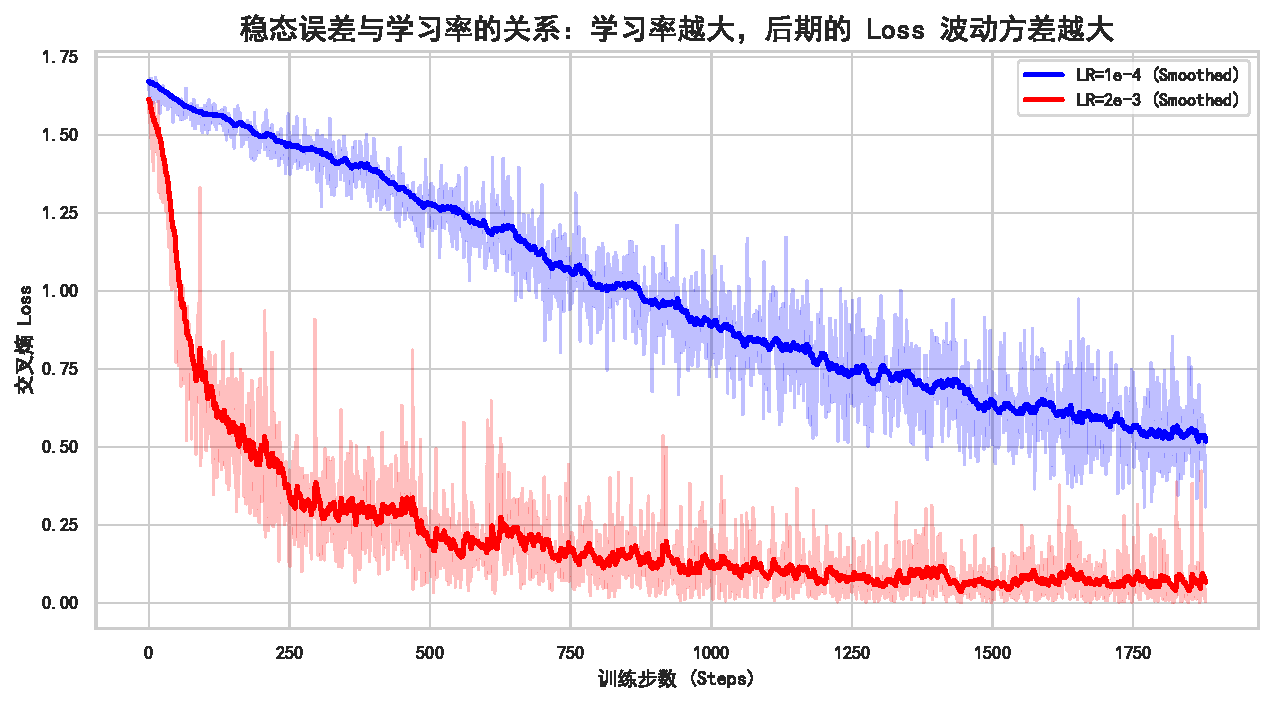
\includegraphics[width=0.8\textwidth]{images/sgd_exp1_lr.pdf}
    \caption{固定 Batch Size，不同学习率对稳态方差的影响}
\end{figure}

\begin{AnalysisBox}{实验结果分析}
通过图表可以直观地观察到，当模型训练逐渐深入，Loss 不再发生显著下降（进入稳态附近），大学习率 ($\eta = 2 \times 10^{-3}$) 的 Loss 曲线出现了极其剧烈的上下振荡。而较小学习率 ($\eta = 10^{-4}$) 的曲线虽有波动，但振幅远小于前者。这完美印证了“梯度方差正比于学习率”的理论。过大的学习率就像在谷底来回剧烈跳跃，使得模型始终无法收敛至精细的局部最优解。
\end{AnalysisBox}

\subsubsection{实验二：稳态方差与 Batch Size 的关系}

接下来，我们固定学习率 $\eta$，改变批次大小 $B$。较大的 $B$ 意味着我们在一次迭代中使用了更多的数据来估计真实梯度，因此梯度的估计会更加准确，随机噪声减少，表现为 Loss 曲线的平滑。

\begin{CodeBox}{Python}[实验二代码]
\begin{lstlisting}[style=PythonStyle]
# 固定学习率，对比 Batch Size。缩短 epoch 即可快速看到由于 Batch Size 带来的前期振荡差异。
res_bs_small = run_experiment(batch_size=16, lr=5e-4, epochs=4)
res_bs_large = run_experiment(batch_size=128, lr=5e-4, epochs=4)

df_bs_small = pd.DataFrame(res_bs_small)
df_bs_small['Batch Size'] = '16 (较小)'
df_bs_large = pd.DataFrame(res_bs_large)
df_bs_large['Batch Size'] = '128 (较大)'
df_exp2 = pd.concat([df_bs_small, df_bs_large])

# 绘图逻辑省略，保存为 sgd_exp2_bs.pdf
\end{lstlisting}
\end{CodeBox}

\begin{OutputBox}
(已成功生成并保存训练损失曲线对比图：\texttt{images/exp2\_bs.pdf})
\end{OutputBox}

\begin{figure}[H]
    \centering
    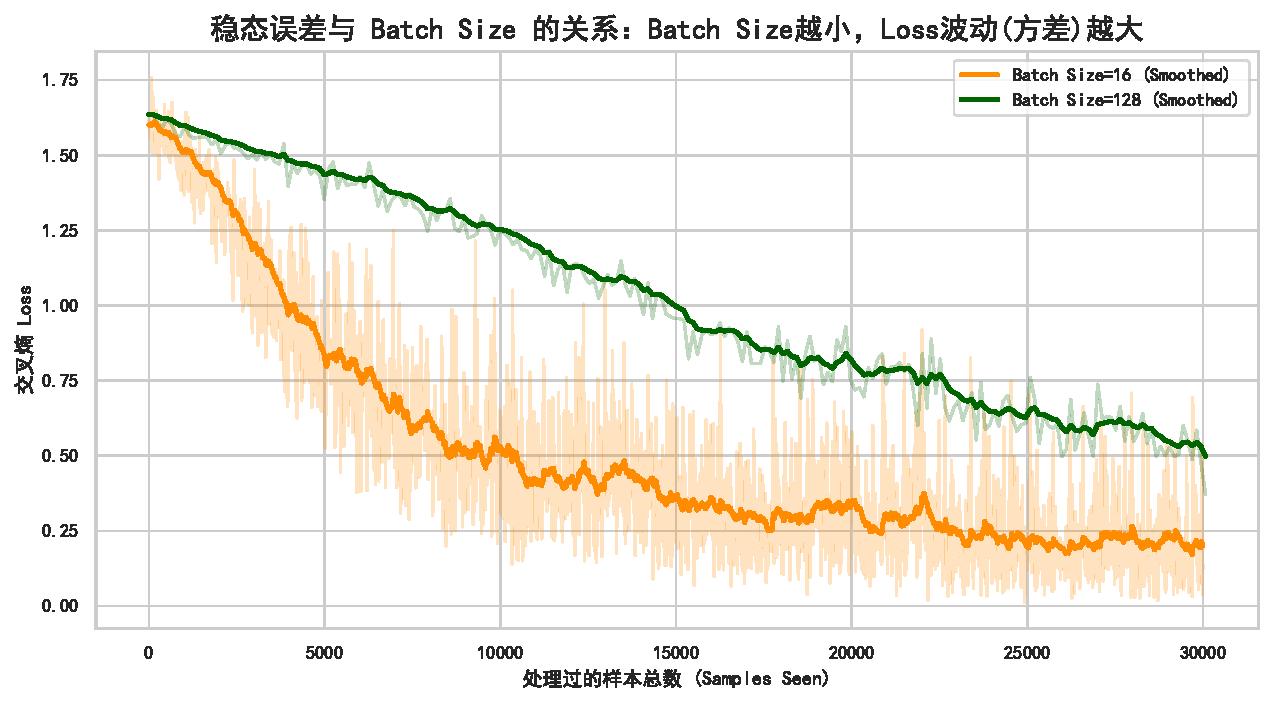
\includegraphics[width=0.8\textwidth]{images/sgd_exp2_bs.pdf}
    \caption{固定学习率，不同 Batch Size 对梯度噪声的影响}
\end{figure}

\begin{AnalysisBox}{实验结果分析}
在图表中，Batch Size=128 的橘色曲线明显比 Batch Size=16 的蓝色曲线平滑得多。小批次由于包含的样本较少，无法准确代表全局数据的分布，进而产生强烈的“随机性”与“抖动”现象。理论公式 $\displaystyle V_{\infty} \propto \frac{\eta}{B}$ 中分母变大导致方差变小，此现象在此展现得淋漓尽致。
\end{AnalysisBox}

\subsubsection{实验三：学习率与 Batch Size 的线性缩放法则}

在分布式训练中，我们往往为了加快训练速度而增大 Batch Size。根据前文推导，为了保证优化器经历相同的噪声分布规律以及同样的进度，当我们将 Batch Size 扩大 $k$ 倍时，学习率原则上也应扩大 $k$ 倍，即线性缩放法则（Linear Scaling Rule）。

\begin{CodeBox}{Python}[实验三代码]
\begin{lstlisting}[style=PythonStyle]
# 基准组：B=16, lr=2e-4
res_base = run_experiment(batch_size=16, lr=2e-4, epochs=5)
# 缩放组：B扩大4倍至64，同时 lr 也扩大4倍至8e-4
res_scaled = run_experiment(batch_size=64, lr=8e-4, epochs=5)

df_base = pd.DataFrame(res_base)
df_base['Setting'] = 'Base (B=16, lr=2e-4)'
df_scaled = pd.DataFrame(res_scaled)
df_scaled['Setting'] = 'Scaled (B=64, lr=8e-4)'
df_exp3 = pd.concat([df_base, df_scaled])

# 绘图逻辑省略，保存为 sgd_exp3_scaling.pdf
\end{lstlisting}
\end{CodeBox}

\begin{OutputBox}
(已成功生成并保存训练损失曲线对比图：\texttt{images/exp3\_scale.pdf})
\end{OutputBox}

\begin{figure}[H]
    \centering
    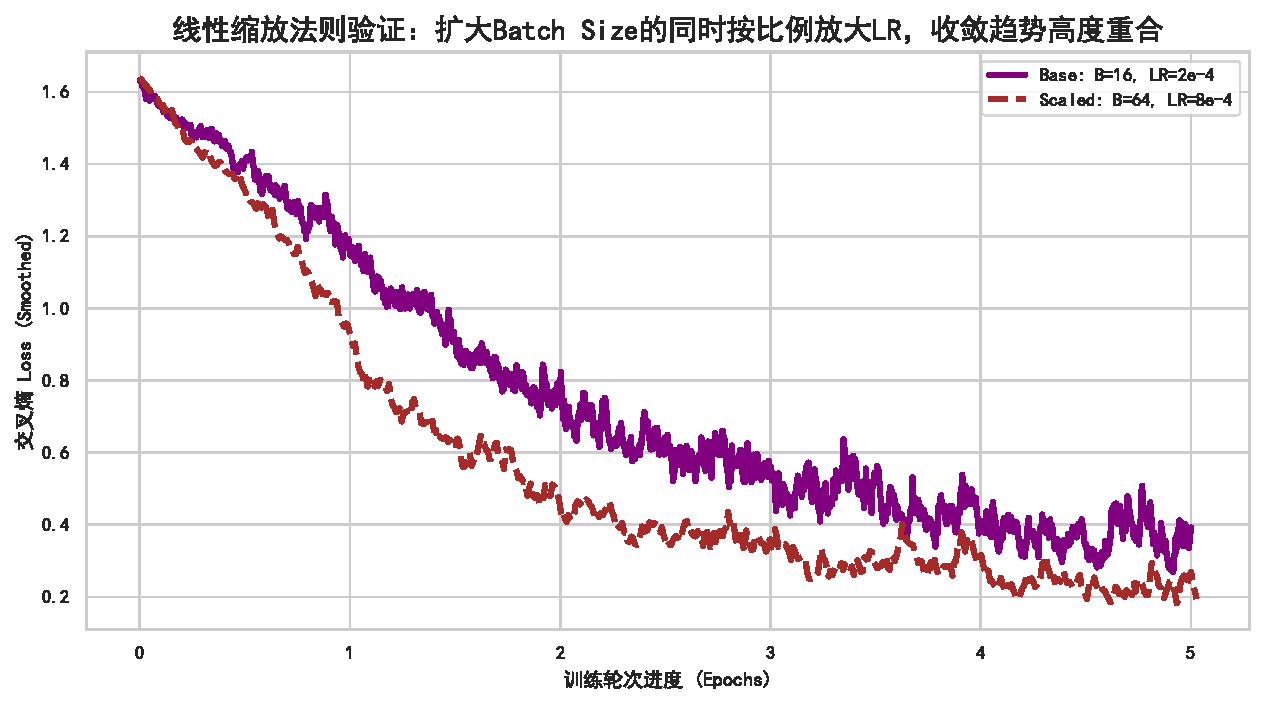
\includegraphics[width=0.8\textwidth]{images/sgd_exp3_scaling.pdf}
    \caption{应用线性缩放法则的 Loss 曲线重合对比}
\end{figure}

\begin{AnalysisBox}{实验结果分析}
令人惊叹的是，两条采用了完全不同超参数配置的曲线，其下降趋势与振幅范围高度吻合。当 $B$ 扩大时减少了方差，但同时 $\eta$ 的等比例扩大又补足了这部分方差。此时每一步更新的预期步长保持等效。这一实验直接验证了“Linear Scaling Rule”在大规模并行分布式训练中的核心指导意义。
\end{AnalysisBox}

\subsubsection{实验四：学习率衰减（LR Decay）对偏差-方差的阶段性影响}

最后，我们探究由于引入学习率衰减所带来的“偏差”与“方差”的此消彼长。在训练初期我们需要大学习率来降低偏差（快速冲向山谷），在后期我们需要小学习率来降低方差（稳固停在谷底）。

\begin{CodeBox}{Python}[实验四代码]
\begin{lstlisting}[style=PythonStyle]
# 常数学习率组 vs. 学习率衰减组
res_constant = run_experiment(batch_size=32, lr=1e-3, epochs=8, use_scheduler=False)
res_decay = run_experiment(batch_size=32, lr=1e-3, epochs=8, use_scheduler=True)

df_const = pd.DataFrame(res_constant)
df_const['Strategy'] = 'Constant LR'
df_dec = pd.DataFrame(res_decay)
df_dec['Strategy'] = 'Cosine Decay LR'
df_exp4 = pd.concat([df_const, df_dec])

# 绘图逻辑省略，保存为 sgd_exp4_decay.pdf
\end{lstlisting}
\end{CodeBox}

\begin{OutputBox}
(已成功生成并保存训练损失曲线对比图：\texttt{images/exp4\_decay.pdf})
\end{OutputBox}

\begin{figure}[H]
    \centering
    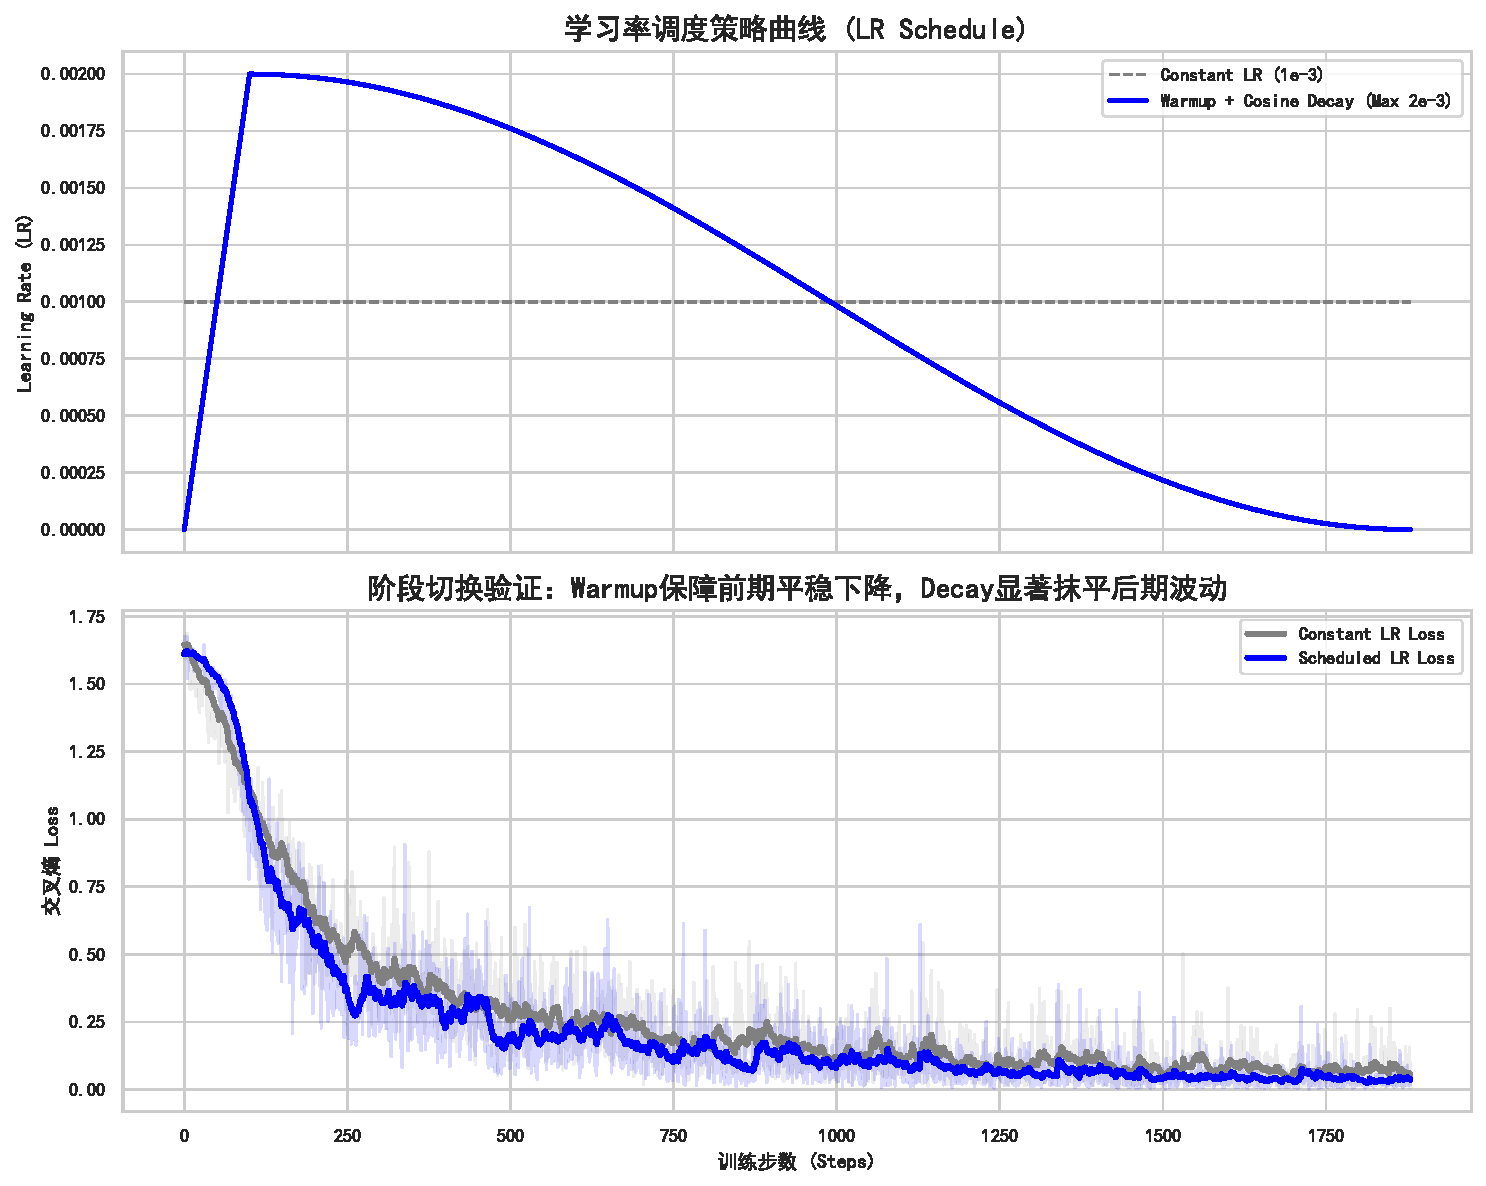
\includegraphics[width=0.6\textwidth]{images/sgd_exp4_decay.pdf}
    \caption{学习率衰减对比：降低稳态方差的有效策略}
\end{figure}

\begin{AnalysisBox}{实验结果分析}
在训练的前几个 epoch 中，由于 Cosine Annealing 衰减处于早期，两者学习率相差不大，Loss 下降的速率基本一致（偏差主导阶段快速下降）。
但是，当训练步入中后期，常数学习率组因为固定的高 $\eta$，出现了明显的上下震荡，模型无法继续收敛；而采用衰减策略的曲线则随着学习率的缩小，振幅大幅下降，其最终落点比常数学习率组更低。这说明了 LR Decay 是一个逐步压低方差、帮助模型向谷底收拢的必要技巧。
\end{AnalysisBox}

\subsection{Regret理论：对学习全过程进行监控（未完待续）}
\subsection{Warmup:训练前期的学习率优化方案}
\subsection{NKT、μP理论：大规模算力下的优化策略}
\end{document}
